\documentclass[
  shortnames]{jss}

\usepackage[utf8]{inputenc}

\author{
Michael Dumelle\\United States\\
Environmental Protection Agency \And Tom Kincaid\\United States\\
Environmental Protection Agency \AND Anthony R. Olsen\\United States\\
Environmental Protection Agency \And Marc Weber\\United States\\
Environmental Protection Agency
}
\title{\pkg{spsurvey}: Spatial Sampling Design and Analysis in \proglang{R}}

\Plainauthor{Michael Dumelle, Tom Kincaid, Anthony R. Olsen, Marc Weber}
\Plaintitle{spsurvey: Spatial Sampling Design and Analysis in R}
\Shorttitle{\pkg{spsurvey}: Spatial Sampling Design and Analysis in \proglang{R}}


\Abstract{
\pkg{spsurvey} is an \proglang{R} package for design-based statistical
inference, with a focus on spatial data. \pkg{spsurvey} provides the
generalized random-tesselation stratified (GRTS) algorithm to select
spatially balanced samples via the \code{grts()} function. The
\code{grts()} function flexibly accomodates several sampling design
features, including stratification, varying inclusion probabilities,
legacy (or historical) sites, minimum distances between sites, and two
options for replacement sites. \pkg{spsurvey} also provides a suite of
data analysis options, including categorical variable analysis
(\code{cat\_analysis()}), continuous variable analysis
(\code{cont\_analysis()}), relative risk analysis
(\code{relrisk\_analysis()}), attributable risk analysis
(\code{attrisk\_analysis()}), difference in risk analysis
(\code{diffrisk\_analysis()}), change analysis
(\code{change\_analysis()}), and trend analysis
(\code{trend\_analysis()}). In this manuscript, we first provide
background for the GRTS algorithm and the analysis approaches and then
show how to implement them in \pkg{spsurvey}. We find that the spatially
balanced GRTS algorithm yields more precise parameter estimates than
simple random sampling, which ignores spatial information.
}

\Keywords{design-based inference, generalized random-tessellation stratified algorithm, Horvitz-Thompson, inclusion probability, spatial balance, variance estimation}
\Plainkeywords{design-based inference, generalized random-tessellation stratified algorithm, Horvitz-Thompson, inclusion probability, spatial balance, variance estimation}

%% publication information
%% \Volume{50}
%% \Issue{9}
%% \Month{June}
%% \Year{2012}
%% \Submitdate{}
%% \Acceptdate{2012-06-04}

\Address{
    Michael Dumelle\\
    United States Environmental Protection Agency\\
    200 SW 35th St\\
Corvallis, OR 97330\\
  E-mail: \email{Dumelle.Michael@epa.gov}\\
  URL: \url{https://CRAN.R-project.org/package=spsurvey}\\~\\
        }


% tightlist command for lists without linebreak
\providecommand{\tightlist}{%
  \setlength{\itemsep}{0pt}\setlength{\parskip}{0pt}}




\usepackage{amsmath} \usepackage{caption} \usepackage{subcaption} \usepackage{color} \usepackage{lineno}

\begin{document}



\linenumbers

\hypertarget{sec:introduction}{%
\section{Introduction}\label{sec:introduction}}

Survey designs are often used to study an environmental resource in a
population. These populations are comprised of individual population
units, which are often referred to as sites. Each site contains
information about the environmental resource, and a complete
characterization of the resource can be obtained by studying every site.
Unfortunately, studying every site is rarely feasible. Therefore, a
sample of sites is collected, and the sample is used to make
generalizations about the larger population. Typically sites are
selected without replacement, and we make this assumption henceforth.
The process by which sites are selected in the sample is known as the
sampling design.

In the design-based approach to statistical inference, a sample should
be representative of the population, but the term representative is
often vague and has multiple interpretations
\citep{kruskal1979representativea, kruskal1979representativeb, kruskal1979representativec}.
We claim a representative sample should have at least the following two
properties. First, the sites must be selected as part of the sample via
a random mechanism. The design-based approach to statistical inference
relies on a random selection of sites; the random site selection forms
the foundation for deriving properties of parameter estimates
\citep{sarndal2003model, lohr2009sampling}. Second, the probability each
site is selected as part of the sample is greater than zero. This
probability of selection is known as an inclusion probability.

There are three types of commonly studied environmental resources: point
resources, linear resources, and areal resources. A point resource has a
finite number of population units (i.e., a finite population) and
represents a collection of point geometries. An example of a point
resource is all lakes (viewed as a whole) in the United States, using
the centroid of the lake as the site location. A linear resource has an
infinite number of population units (i.e., an infinite population) and
represents a collection of linestring geometries. An example of a linear
resource is all streams in the United States. An areal resource has an
infinite number of population units and represents a collection of
polygon geometries. An example of an areal resource is the San Francisco
Bay Estuary.

These point, linear, and areal resources tend to be spread over
geographic space. If a sample is well-spread over geographic space, we
call it a spatially balanced sample (we provide a more technical
definition of spatial balance in
Section\(~\)\ref{subsec:grts_algorithm}). Spatially balanced samples are
desirable because they tend to yield more precise parameter estimates
than samples that are not spatially balanced
\citep{stevens2004grts, barabesi2011sampling, grafstrom2013well, robertson2013bas, wang2013design, benedetti2017spatiallyreview}.

The \pkg{spsurvey} package selects spatially balanced samples using the
generalized random-tessellation stratified (GRTS) algorithm
\citep{stevens2004grts}. Shortly after the GRTS algorithm emerged,
several other spatially balanced sampling algorithms followed.
\citet{walvoort2010r} used compact geographical strata to perform
stratified sampling; this approach is available in the \pkg{spcosa}
\proglang{R} package. \citet{grafstrom2012spatially} used a local pivot
method for finite populations and \citet{grafstrom2018spatially}
generalized this approach to infinite populations; these approaches are
available in the \pkg{BalancedSampling} \proglang{R} package
\citep{grafstrom2019BalancedSampling}.
\citet{grafstrom2012spatiallypoisson} used a spatially correlated
Poisson approach, also available in \pkg{BalancedSampling}.
\citet{benedetti2017spatially} used a within-sample distance approach
available in the \pkg{Spbsampling} \proglang{R} package
\citep{pantalone2022spbsampling}. \citet{robertson2013bas} developed
balanced acceptance sampling, and subsequently,
\citet{robertson2018halton} used Halton iterative partitioning; these
approaches are available in the \pkg{SDraw} \proglang{R} package
\citep{mcdonald2020SDraw}. \citet{foster2020spatially} developed
spatially balanced transect sampling; this approach is available in the
\pkg{MBHdesign} \proglang{R} package \citep{foster2021mbhdesign}.

The GRTS algorithm in \pkg{spsurvey} implements many features absent
from the aforementioned software packages. The GRTS algorithm in
\pkg{spsurvey} can be applied to all three resource types: point,
linear, and areal. It accommodates several sampling design features like
stratification, unequal selection probabilities, legacy (or historical)
sites, minimum distances between sites, and two options for replacement
sites (reverse hierarchical ordering and nearest neighbor). The GRTS
algorithm is discussed in more detail in Section\(~\)\ref{sec:design}.
Section\(~\)\ref{sec:design} also showcases how \pkg{spsurvey} can be
used to summarize and visualize sampling frames and samples as well as
measure spatial balance.

Another benefit of \pkg{spsurvey} compared to the aforementioned
software packages is that \pkg{spsurvey} can also be used to analyze
data and estimate parameters of a population. \pkg{spsurvey} has a suite
of analysis functions that enable categorical variable analysis,
continuous variable analysis, attributable risk analysis, relative risk
analysis, difference in risk analysis, change analysis, and trend
analysis. In addition, variances can be estimated using the local
neighborhood variance estimator \citep{stevens2003variance}, which
increases precision by using the spatial locations of each observation
in variance estimation. The analysis functions in \pkg{spsurvey} are
discussed in more detail in Section\(~\)\ref{sec:analysis}.

The rest of this paper is organized as follows. In
Section\(~\)\ref{sec:design}, we review spatially balanced sampling in
\pkg{spsurvey}. In Section\(~\)\ref{sec:analysis}, we the describe the
analysis approaches available in \pkg{spsurvey}. In
Section\(~\)\ref{sec:application}, we compare performance of the GRTS
algorithm and local neighborhood variance estimator to simple random
sampling using data from the 2012 National Lakes Assessment
\citep{usepa2012NLA}. And in Section\(~\)\ref{sec:discussion}, we end
with a discussion and explore potential future developments for
\pkg{spsurvey}.

To install and load \pkg{spsurvey}, run

\begin{CodeChunk}
\begin{CodeInput}
R> install.packages("spsurvey")
R> library("spsurvey")
\end{CodeInput}
\end{CodeChunk}

\hypertarget{sec:design}{%
\section{Spatially balanced sampling}\label{sec:design}}

In Section\(~\)\ref{sec:introduction} we introduced the notion of a
random sample. Random samples are selected from a collection of sites.
This collection of sites is known as the sampling frame. Ideally, the
set of sites in the sampling frame is the same as the set of sites in
the population. Unfortunately this is not always true, as a sampling
frame may contain some sites that are not in the population
(overcoverage), may be missing sites from the population
(undercoverage), or both. Selecting an appropriate sampling frame is
crucial if you want to generalize results from the sample to the
population. To understand whether a sampling frame is appropriate for a
population, summaries and visualizations of the sampling frame are
helpful. Next we demonstrate using \pkg{spsurvey} to summarize and
visualize sampling frames. We then give theoretical background for the
generalized random-tessellation stratified (GRTS) algorithm and show how
to use it in \pkg{spsurvey} to select spatially balanced samples and to
summarize, visualize, write, and print these samples. We end the section
by showing how to explicitly measure spatial balance using
\pkg{spsurvey} and to use GRTS for a variety of resource types.

\hypertarget{subsec:sv_sframe}{%
\subsection{Summarizing and visualizing sampling
frames}\label{subsec:sv_sframe}}

Sampling frames for point, linear, or areal resources summarized and
visualized in \pkg{spsurvey} using the \code{summary()} and
\code{plot()} functions, respectively. The \code{summary()} and
\code{plot()} functions have similar syntax and require at least two
arguments: the sampling frame and a formula. The sampling frame must be
an \pkg{sf} object \citep{pebesma2018sf} or a data frame. The formula
specifies the variables in the sampling frame to summarize or visualize
and can be one-sided or two-sided. Additional arguments to
\code{summary()} and \code{plot()} are discussed in more detail later.

To demonstrate the use of \code{summary()} and \code{plot()}, we use the
the \code{NE_Lakes} data in \pkg{spsurvey}. The \code{NE_Lakes} data is
an \pkg{sf} object of 195 lakes in the Northeastern United States. The
\code{NE_Lakes} data represent a point resource, as there are a finite
number of lakes to sample. Later we study linear and areal data in
\pkg{spsurvey}. To load \code{NE_Lakes} into your global environment,
run

\begin{CodeChunk}
\begin{CodeInput}
R> data("NE_Lakes")
\end{CodeInput}
\end{CodeChunk}

There are five variables in \code{NE_Lakes}: \code{AREA}, a continuous
variable representing lake area (in hectares); \code{AREA_CAT}, a
categorical variable representing lake area levels small (1 to 10
hectares) and large (greater than 10 hectares); \code{ELEV}, a
continuous variable representing lake elevation (in meters); and
\code{ELEV_CAT}, a categorical variable representing lake elevation
levels low (0 to 100 meters) and high (greater than 100 meters). We can
view the geometry information and first few rows of \code{NE_Lakes} by
running

\begin{CodeChunk}
\begin{CodeInput}
R> NE_Lakes
\end{CodeInput}
\begin{CodeOutput}
Simple feature collection with 195 features and 4 fields
Geometry type: POINT
Dimension:     XY
Bounding box:  xmin: 1834001 ymin: 2225021 xmax: 2127632 ymax: 2449985
Projected CRS: NAD83 / Conus Albers
First 10 features:
        AREA AREA_CAT   ELEV ELEV_CAT                geometry
1  10.648825    large 264.69     high POINT (1930929 2417191)
2   2.504606    small 557.63     high POINT (1849399 2375085)
3   3.979199    small  28.79      low POINT (2017323 2393723)
4   1.645657    small 212.60     high POINT (1874135 2313865)
5   7.489052    small 239.67     high POINT (1922712 2392868)
6  86.533725    large 195.37     high POINT (1977163 2350744)
7   1.926996    small 158.96     high POINT (1852292 2257784)
8   6.514217    small  29.26      low POINT (1874421 2247388)
9   3.100221    small 204.62     high POINT (1933352 2368181)
10  1.868094    small  78.77      low POINT (1892582 2364213)
\end{CodeOutput}
\end{CodeChunk}

Notice that the geometry type of \code{NE_Lakes} is \code{POINT}, as
\code{NE_Lakes} represents a point resource.

Before summarizing or visualizing \code{NE_Lakes}, store it as an
\code{sp_frame} object by running

\begin{CodeChunk}
\begin{CodeInput}
R> NE_Lakes <- sp_frame(NE_Lakes)
\end{CodeInput}
\end{CodeChunk}

One-sided formulas are used when the goal is to summarize or visualize
variables individually. To summarize the distribution of \code{ELEV_CAT}
using a one-sided formula, run

\begin{CodeChunk}
\begin{CodeInput}
R> summary(NE_Lakes, formula = ~ ELEV_CAT)
\end{CodeInput}
\begin{CodeOutput}
   total     ELEV_CAT  
 total:195   low :112  
             high: 83  
\end{CodeOutput}
\end{CodeChunk}

The output contains two columns: \code{total} and \code{ELEV_CAT}. The
\code{total} column acts as an ``intercept'' in the formula and returns
the total number of observations in the sampling frame; it can be
omitted by supplying \code{- 1} to the formula. The \code{ELEV_CAT}
column returns the number of lakes in the low and high elevation levels.
The same syntax is used to visualize the spatial distribution of
\code{ELEV_CAT} (Figure\(~\)\ref{fig:elevcat}):

\begin{CodeChunk}
\begin{CodeInput}
R> plot(NE_Lakes, formula = ~ ELEV_CAT)
\end{CodeInput}
\end{CodeChunk}

By default, the formula argument to \code{plot()} is the resulting
plot's title, though this can be changed using the \code{main} argument.

\begin{figure}
\centering
\begin{subfigure}{0.49\textwidth}
  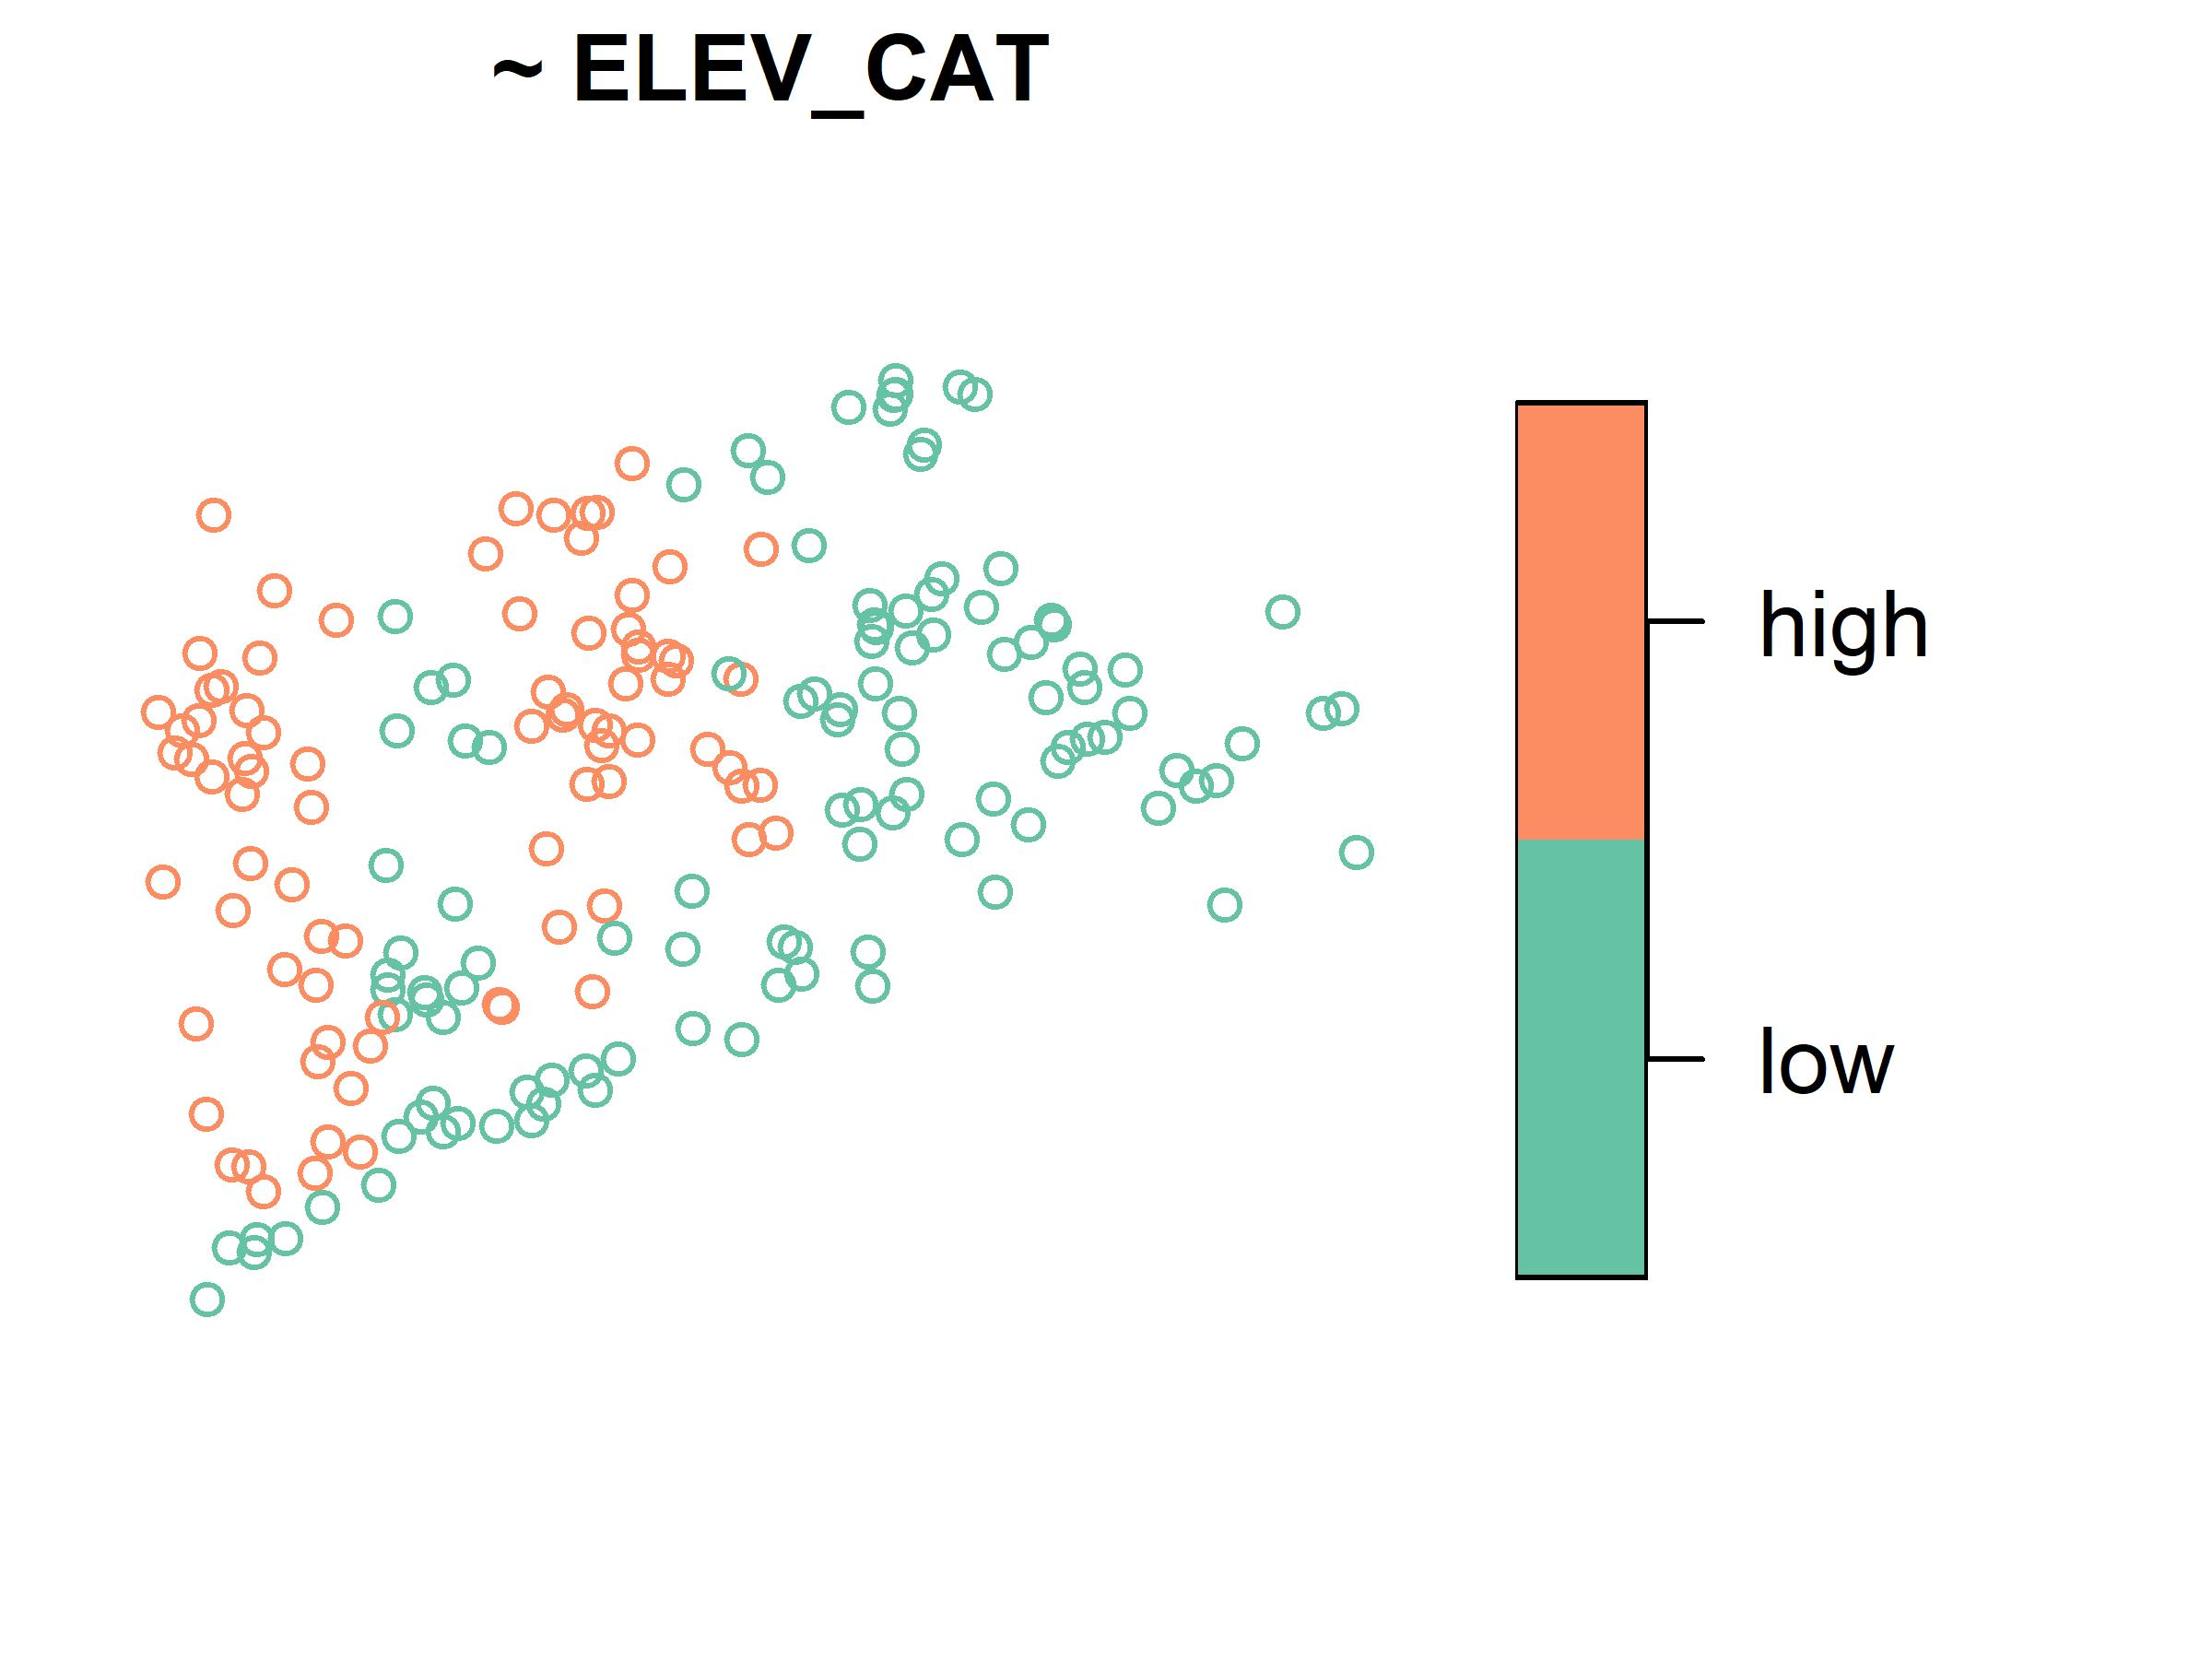
\includegraphics[width = 1\linewidth]{images/elevcat.jpeg}
  \caption{}
  \label{fig:elevcat}
\end{subfigure}
\begin{subfigure}{0.49\textwidth}
  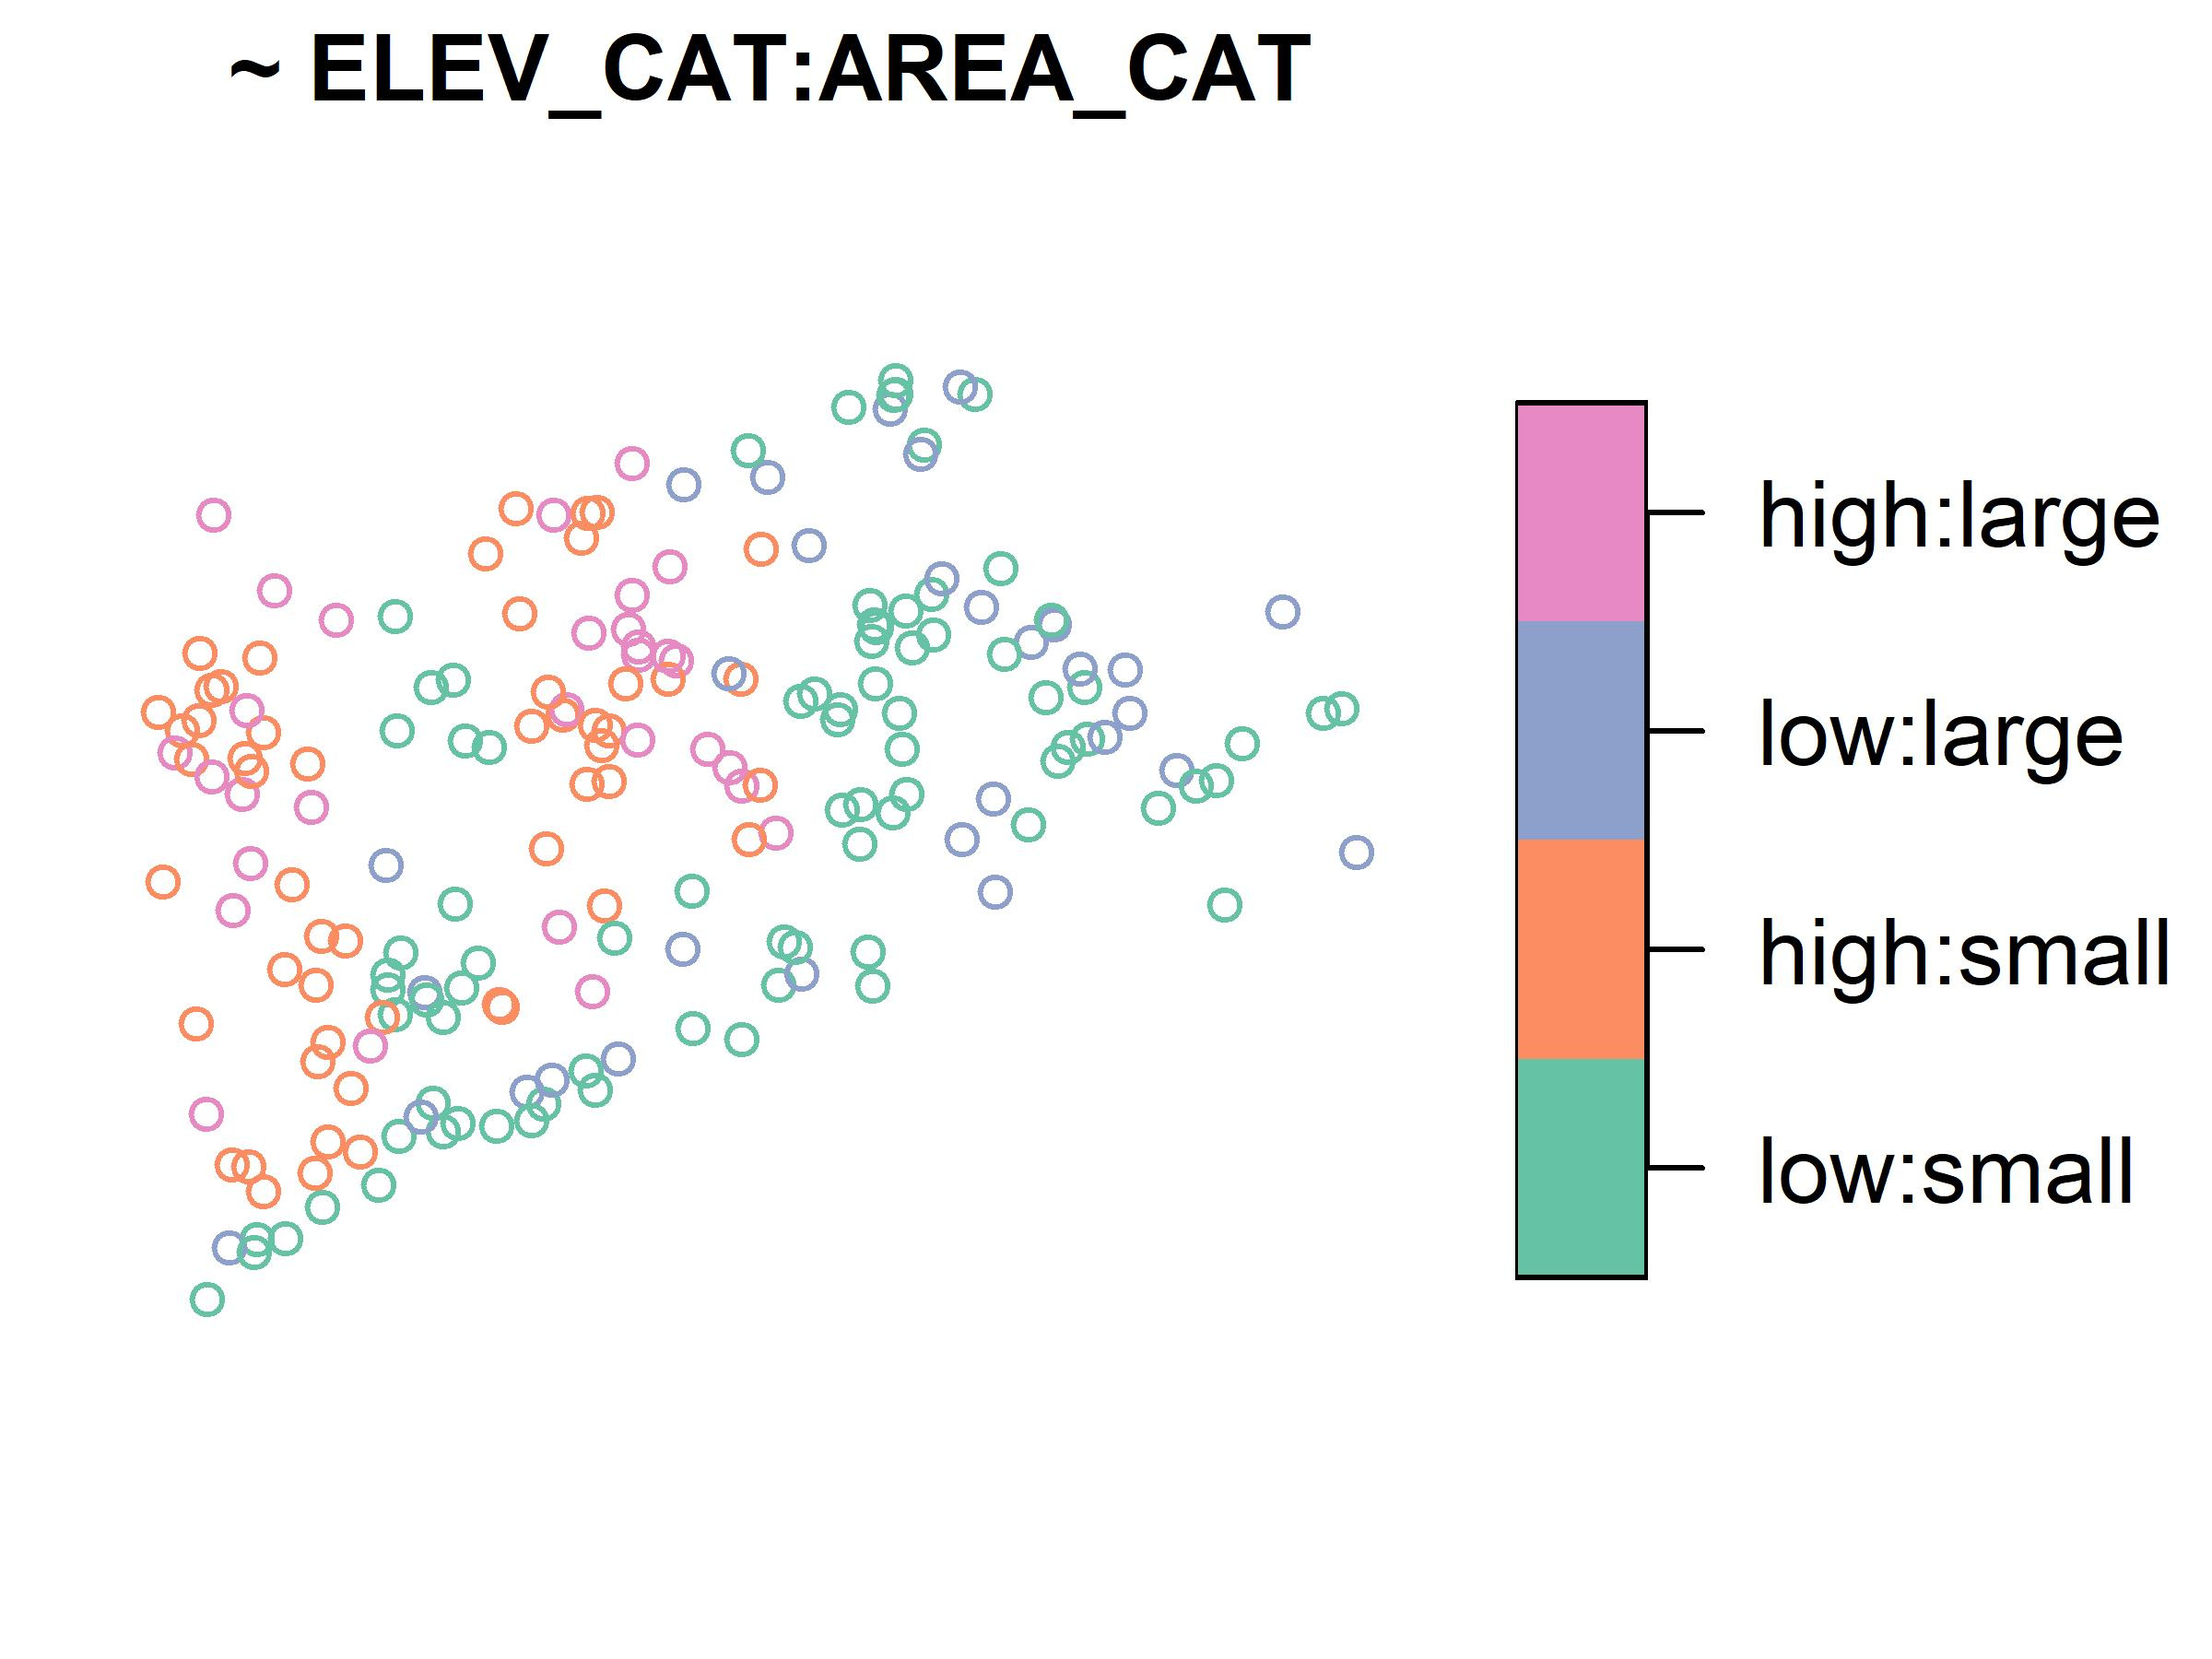
\includegraphics[width = 1\linewidth]{images/elevcat_areacat.jpeg}
  \caption{}
  \label{fig:areacat}
\end{subfigure} 
\caption{Distribution of the lake elevation categories (a) and the interaction between lake elevation categories and lake area categories (b) in the Northeastern lakes data.}
\label{fig:sframes1}
\end{figure}

Additional variables can be added to the formula when separated by
\code{+}. Interactions between variables can be added to the formula
using \texttt{:}. When additional variables are added, \code{summary()}
produces a table-like summary of each variable

\begin{CodeChunk}
\begin{CodeInput}
R> summary(NE_Lakes, formula = ~ ELEV_CAT + ELEV_CAT:AREA_CAT)
\end{CodeInput}
\begin{CodeOutput}
   total     ELEV_CAT    ELEV_CAT:AREA_CAT
 total:195   low :112   low:small :82     
             high: 83   high:small:53     
                        low:large :30     
                        high:large:30     
\end{CodeOutput}
\end{CodeChunk}

Similarly, \code{plot()} produces separate visualizations for each
variable (Figure\(~\)\ref{fig:sframes1}).

\begin{CodeChunk}
\begin{CodeInput}
R> plot(NE_Lakes, formula = ~ ELEV_CAT + ELEV_CAT:AREA_CAT)
\end{CodeInput}
\end{CodeChunk}

These separate visualizations are stepped through using \code{<Return>}.
The \code{summary()} and \code{plot()} functions also support standard
formula syntax shortcuts like \code{.} and \code{*}. The formula
\code{~ .} is shorthand for \code{~ AREA + AREA_CAT + ELEV + ELEV_CAT}
and the formula \code{~ AREA_CAT*ELEV_CAT} is shorthand for
\code{~ AREA_CAT + ELEV_CAT + AREA_CAT:ELEV_CAT}.

Two-sided formulas are useful when the goal is to summarize or visualize
one variable (a left-hand side variable) for each level of other
variables (right-hand side variables). When using two-sided formulas,
\code{summary()} returns table-like summaries of the left-hand side
variable for each level of each right-hand side variable:

\begin{CodeChunk}
\begin{CodeInput}
R> summary(NE_Lakes, formula = ELEV ~ AREA_CAT)
\end{CodeInput}
\begin{CodeOutput}
ELEV by total: 
      Min. 1st Qu. Median     Mean 3rd Qu.   Max.
total    0  21.925  69.09 127.3862 203.255 561.41

ELEV by AREA_CAT: 
      Min. 1st Qu.  Median     Mean  3rd Qu.   Max.
small 0.00   19.64  59.660 117.4473 176.1700 561.41
large 0.01   26.75 102.415 149.7487 241.2025 537.84
\end{CodeOutput}
\end{CodeChunk}

\code{plot()} returns separate visualizations of the left-hand side
variable for each level of each right-hand side variable. For example,

\begin{CodeChunk}
\begin{CodeInput}
R> plot(NE_Lakes, formula = ELEV ~ AREA_CAT)
\end{CodeInput}
\end{CodeChunk}

produces two separate visualizations -- one for each level of
\code{AREA_CAT} (small and large).

The \code{plot()} function has additional arguments that allow for
flexible customization of graphical parameters. The \code{varlevel_args}
(short for ``variable level arguments'') argument adjusts graphical
parameters separately for each level of a categorical variable. The
\code{var_args} (short for ``variable arguments'') argument adjusts
graphical parameters for a numeric variable or simultaneously for all
levels of a categorical variable. The \code{...} argument adjusts
graphical parameters for all variables simultaneously. \pkg{spsurvey}'s
\code{plot()} function is built on top of \pkg{sf}'s \code{plot()}
function. As a result, it takes the same set of graphical parameters
that \pkg{sf}'s \code{plot()} function does and uses the same default
values.

\hypertarget{subsec:grts_algorithm}{%
\subsection{The generalized random-tessellation stratified
algorithm}\label{subsec:grts_algorithm}}

Before discussing the GRTS algorithm, it is important to identify two
distinct types of spatial balance: spatial balance with respect to the
sampling frame and spatial balance with respect to geography. Spatial
balance with respect to the sampling frame measures how closely the
spatial layout of the sample resembles the spatial layout of the
sampling frame. Spatial balance with respect to geography measures the
geographic spread of the sample -- usually the sites in the sample are
spread out over the domain in some equidistant manner but are not meant
to resemble the spatial layout of the sampling frame. While spatial
balance with respect to geography can be useful, spatial balance with
respect to the sampling frame is preferred for design-based inference
because this type of spatial balance is closely linked to inclusion
probabilities, which we discuss in more detail later. Henceforth, when
we refer to spatial balance, we mean spatial balance with respect to the
sampling frame.

\citet{stevens2004grts} created the first widely-used spatially balanced
sampling algorithm known as the GRTS algorithm. The GRTS algorithm has
several attractive properties we discuss throughout this subsection.
Most notably, the GRTS algorithm accommodates all three resource types:
point, linear, and areal. It also accommodates a suite of flexible
sampling design options like stratification, unequal inclusion
probabilities, legacy (historical) sites, a minimum distance between
sites, and two options for replacement sites. Next we provide a brief
overview of the technical details of the algorithm as described by
\citet{stevens2004grts}.

The first step in the GRTS algorithm is to determine the probability
that each site is selected in the sample, known as an inclusion
probability. For example, if the population size \(N\) equals 100, the
sample size \(n\) equals 10, and each site is equally likely to be
selected in the sample, then each site's inclusion probability is
\(n / N = 10/100 = 0.1\). After determining these inclusion
probabilities, a square bounding box is superimposed onto the sampling
frame. That bounding box is divided into four distinct, equally sized
square cells. These cells compose the first level of a hierarchical grid
and are called level-one cells. These level-one cells are randomly
assigned a level-one address of zero, one, two, or three. The set of
level-one cells is denoted by \(\mathcal{A}_1\) and defined as
\(\mathcal{A}_1 \equiv \{a_1: a_1 = 0, 1, 2, 3\}\)
(Figure\(~\)\ref{fig:grts_level1}). Each level-one cell has an inclusion
value that equals the sum of the inclusion probabilities for the sites
contained in the level-one cell. If any of the level-one cell's
inclusion values are larger than one, a second level of cells is added
by splitting each level-one cell into four distinct, equally sized
squares. Together these small squares compose the second level of a
hierarchical grid and are called level-two cells. Within each level-one
cell, the level-two cells are randomly assigned a level-two address of
zero, one, two, or three. The level-one and level-two addresses compose
a set that can be used to identify any level-two cell. The set of
level-two cells is denoted by \(\mathcal{A}_2\) and defined as
\(\mathcal{A}_2 \equiv \{a_1a_2: a_1 = 0, 1, 2, 3; a_2 = 0, 1, 2, 3\}\)
(Figure\(~\)\ref{fig:grts_level2}). If any of the level-two cell's
inclusion values are greater than one, a third level of cells is added.
This process continues for \(k\) levels, where \(k\) is the first level
that all level-\(k\) cells have inclusion values no greater than one.
Then
\(\mathcal{A}_k \equiv \{a_1...a_k : a_1 = 0, 1, 2, 3; ...; a_k = 0, 1, 2, 3\}\).
This addressing composes a base-four ordering scheme --
\citet{stevens2004grts} provide further details.

\begin{figure}
\centering
\begin{subfigure}{0.45\textwidth}
  \centering
  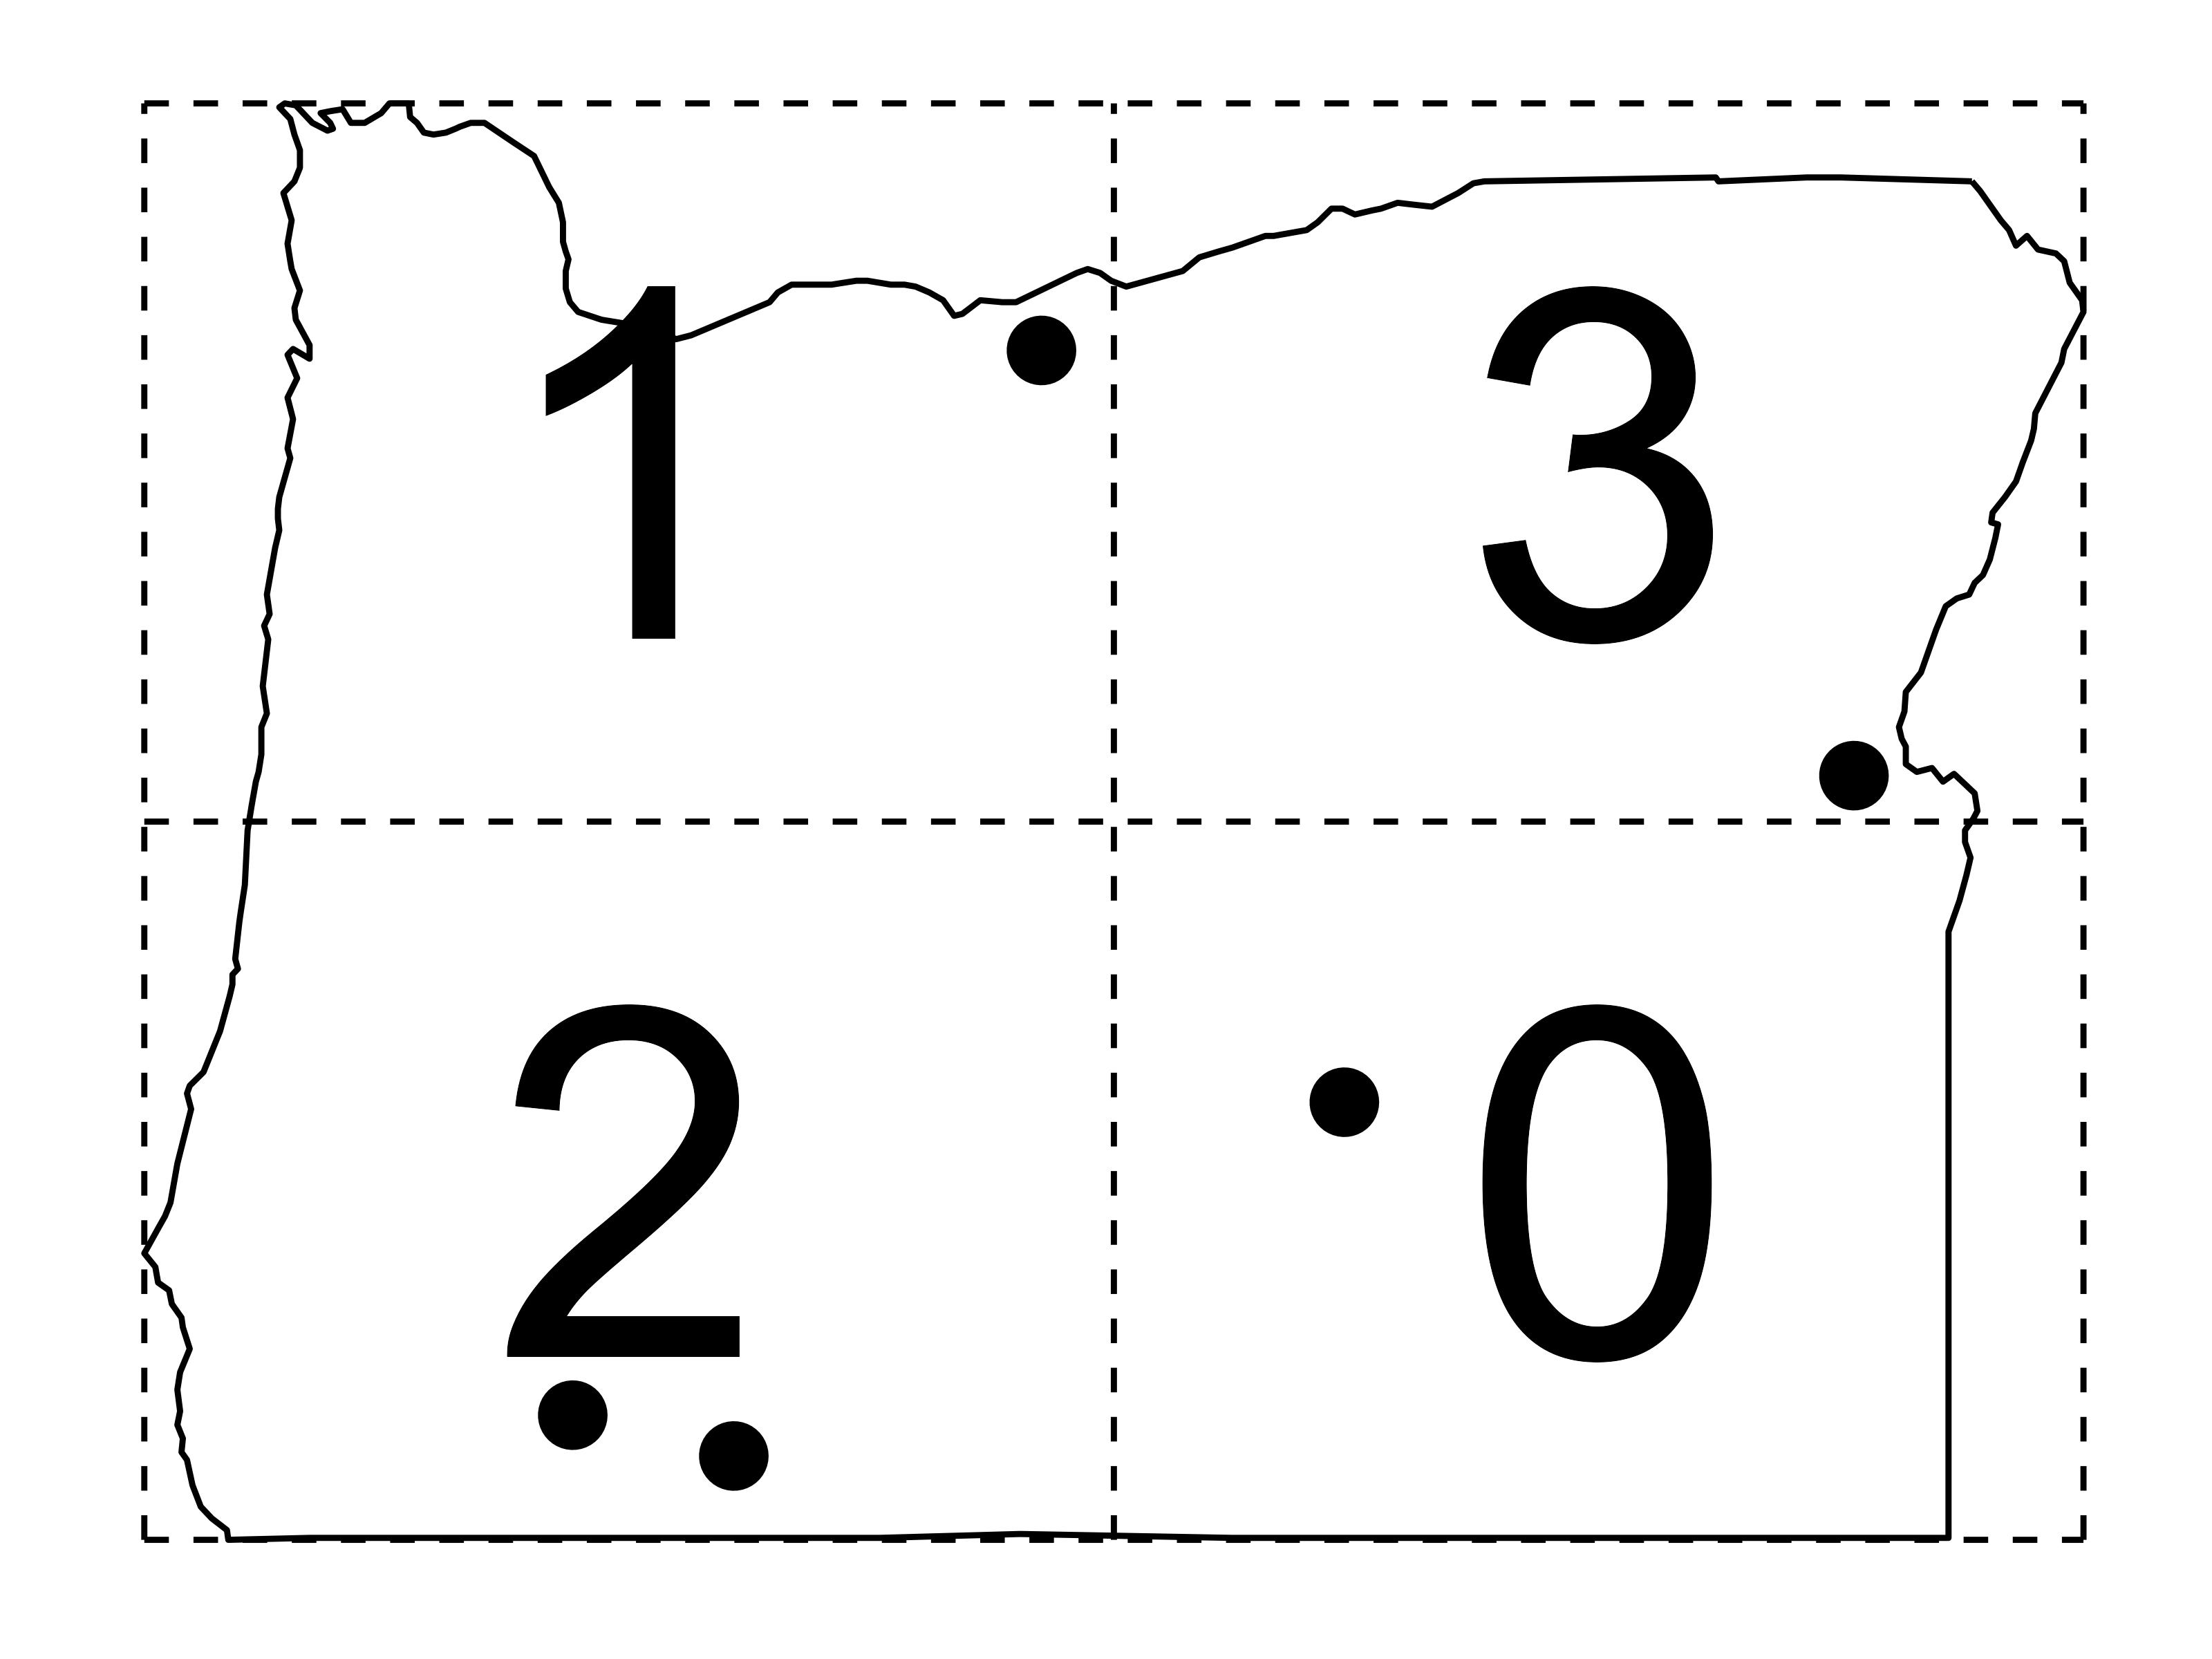
\includegraphics[width = 1\linewidth]{images/grts_level1.jpeg}
  \caption{}
  \label{fig:grts_level1}
\end{subfigure}
\begin{subfigure}{0.45\textwidth}
  \centering
  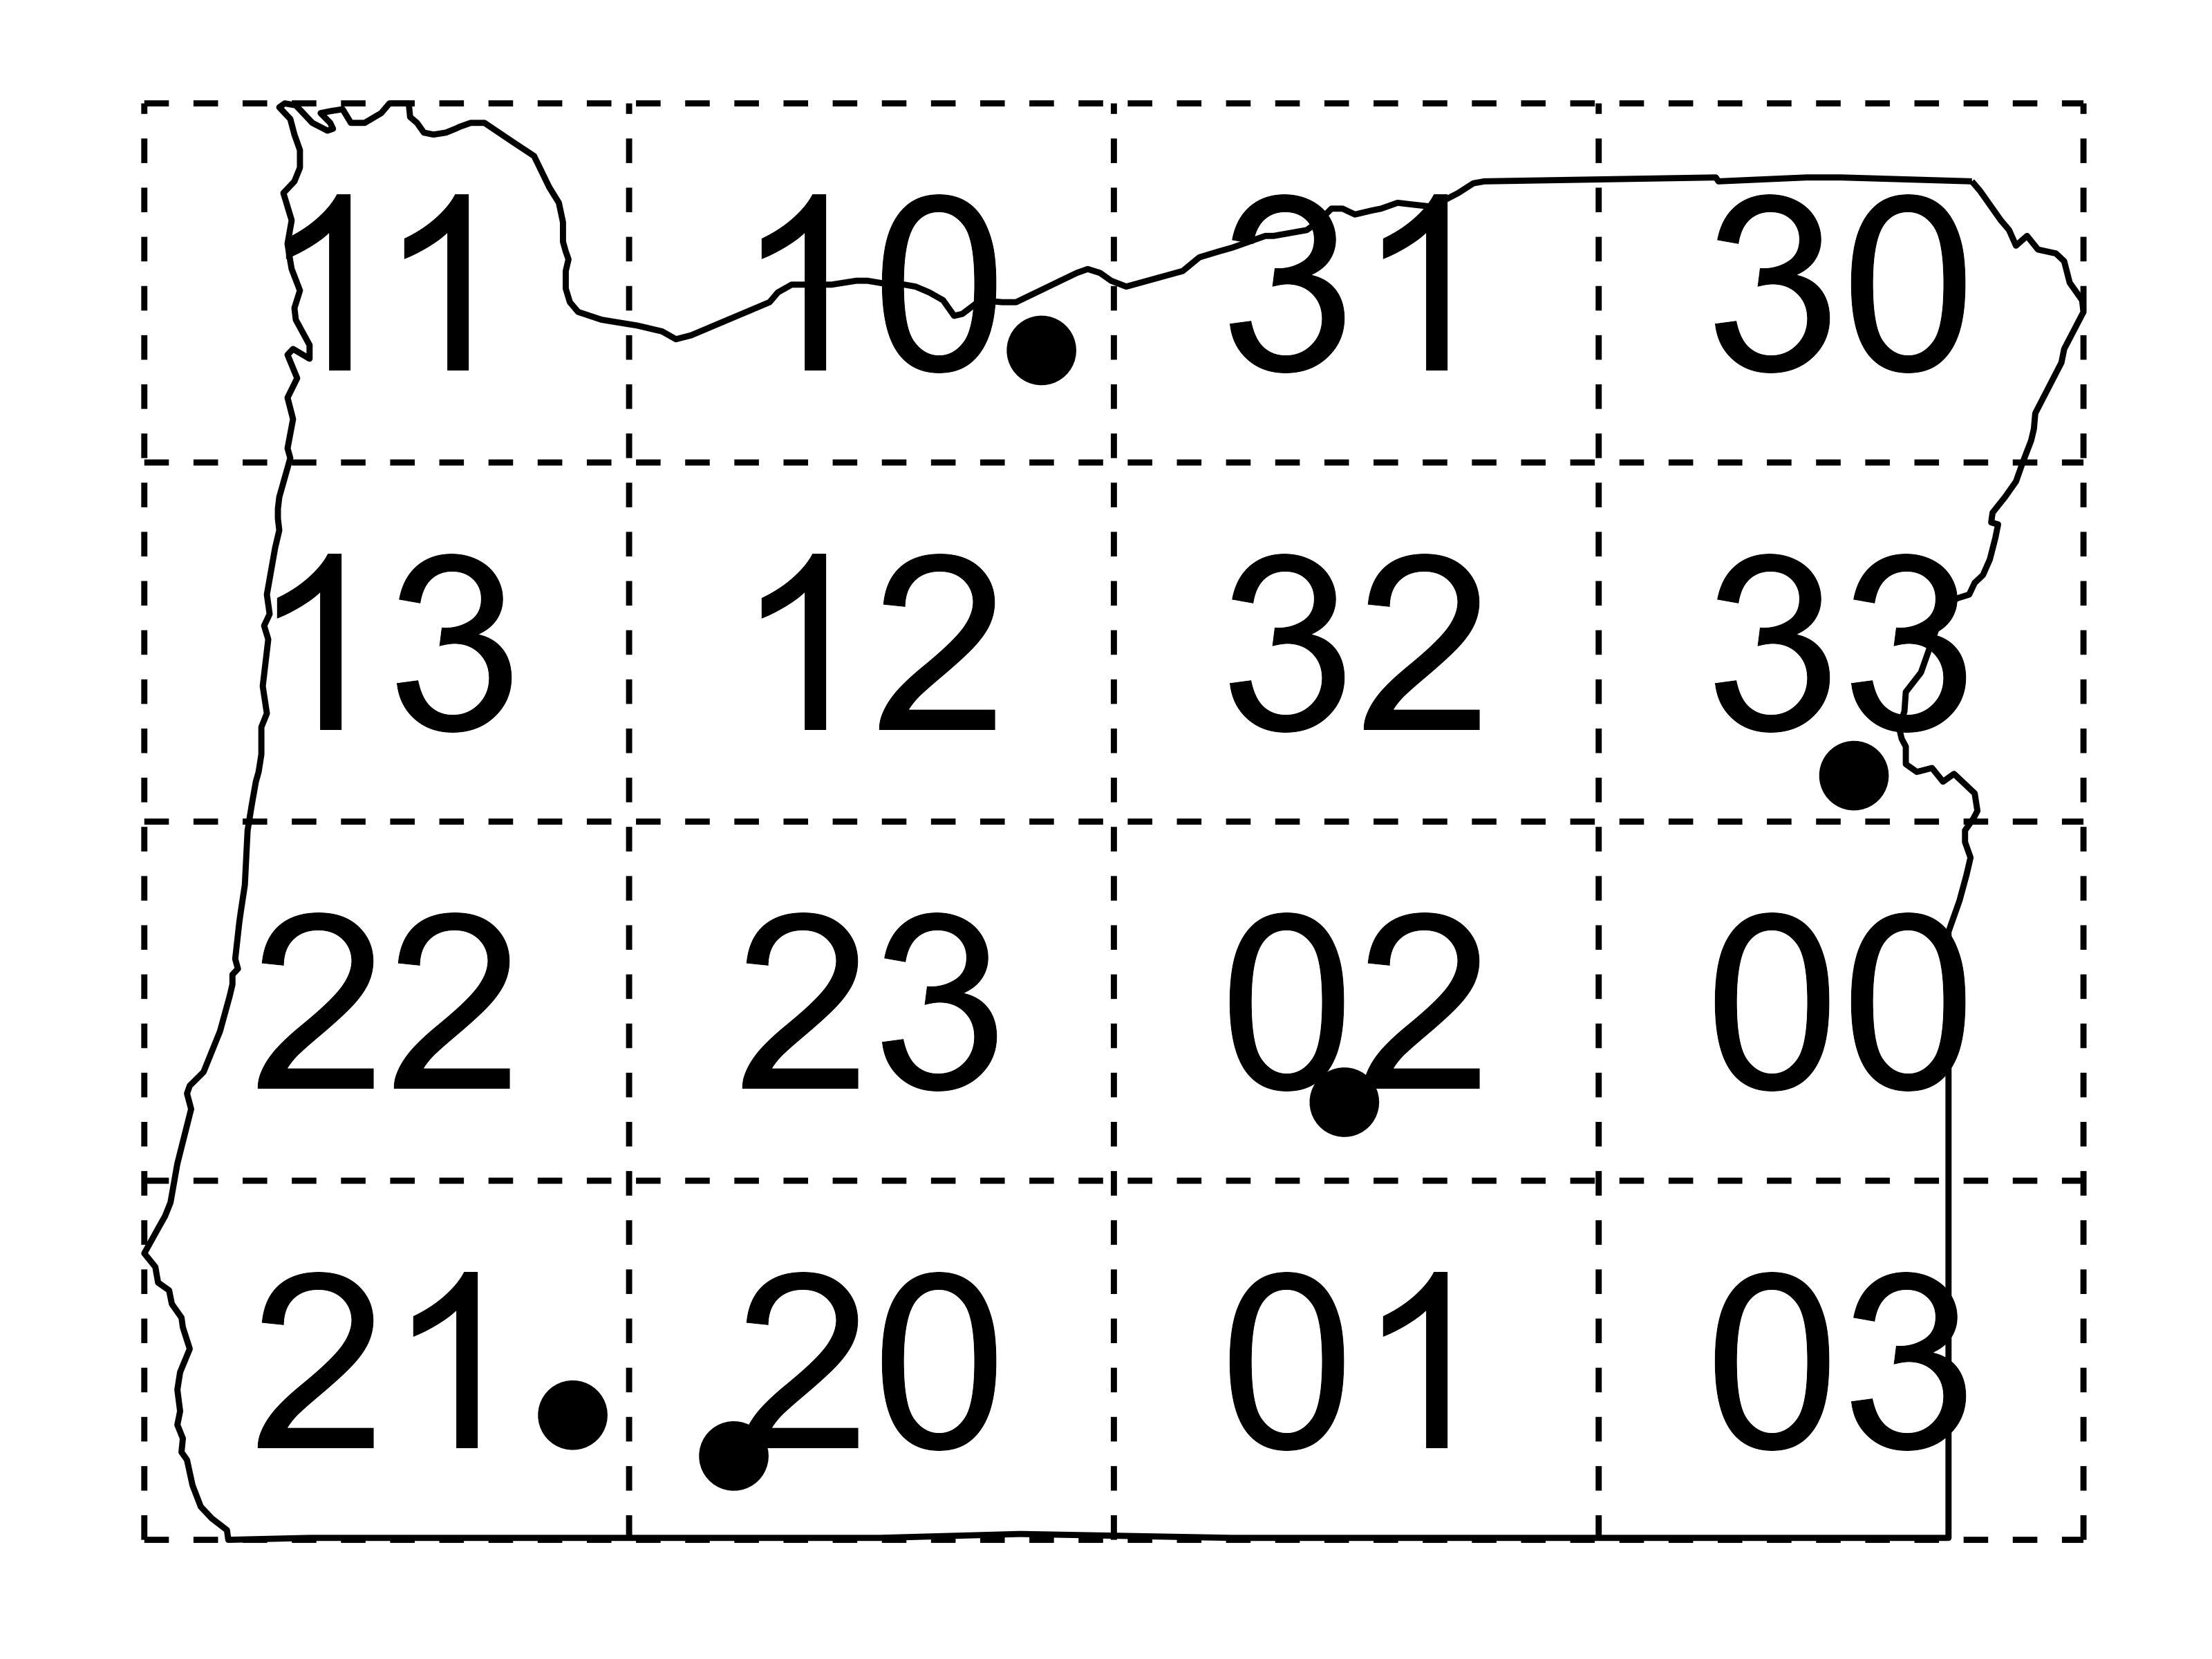
\includegraphics[width = 1\linewidth]{images/grts_level2.jpeg}
  \caption{}
  \label{fig:grts_level2}
\end{subfigure} \\
\begin{subfigure}{0.45\textwidth}
  \centering
  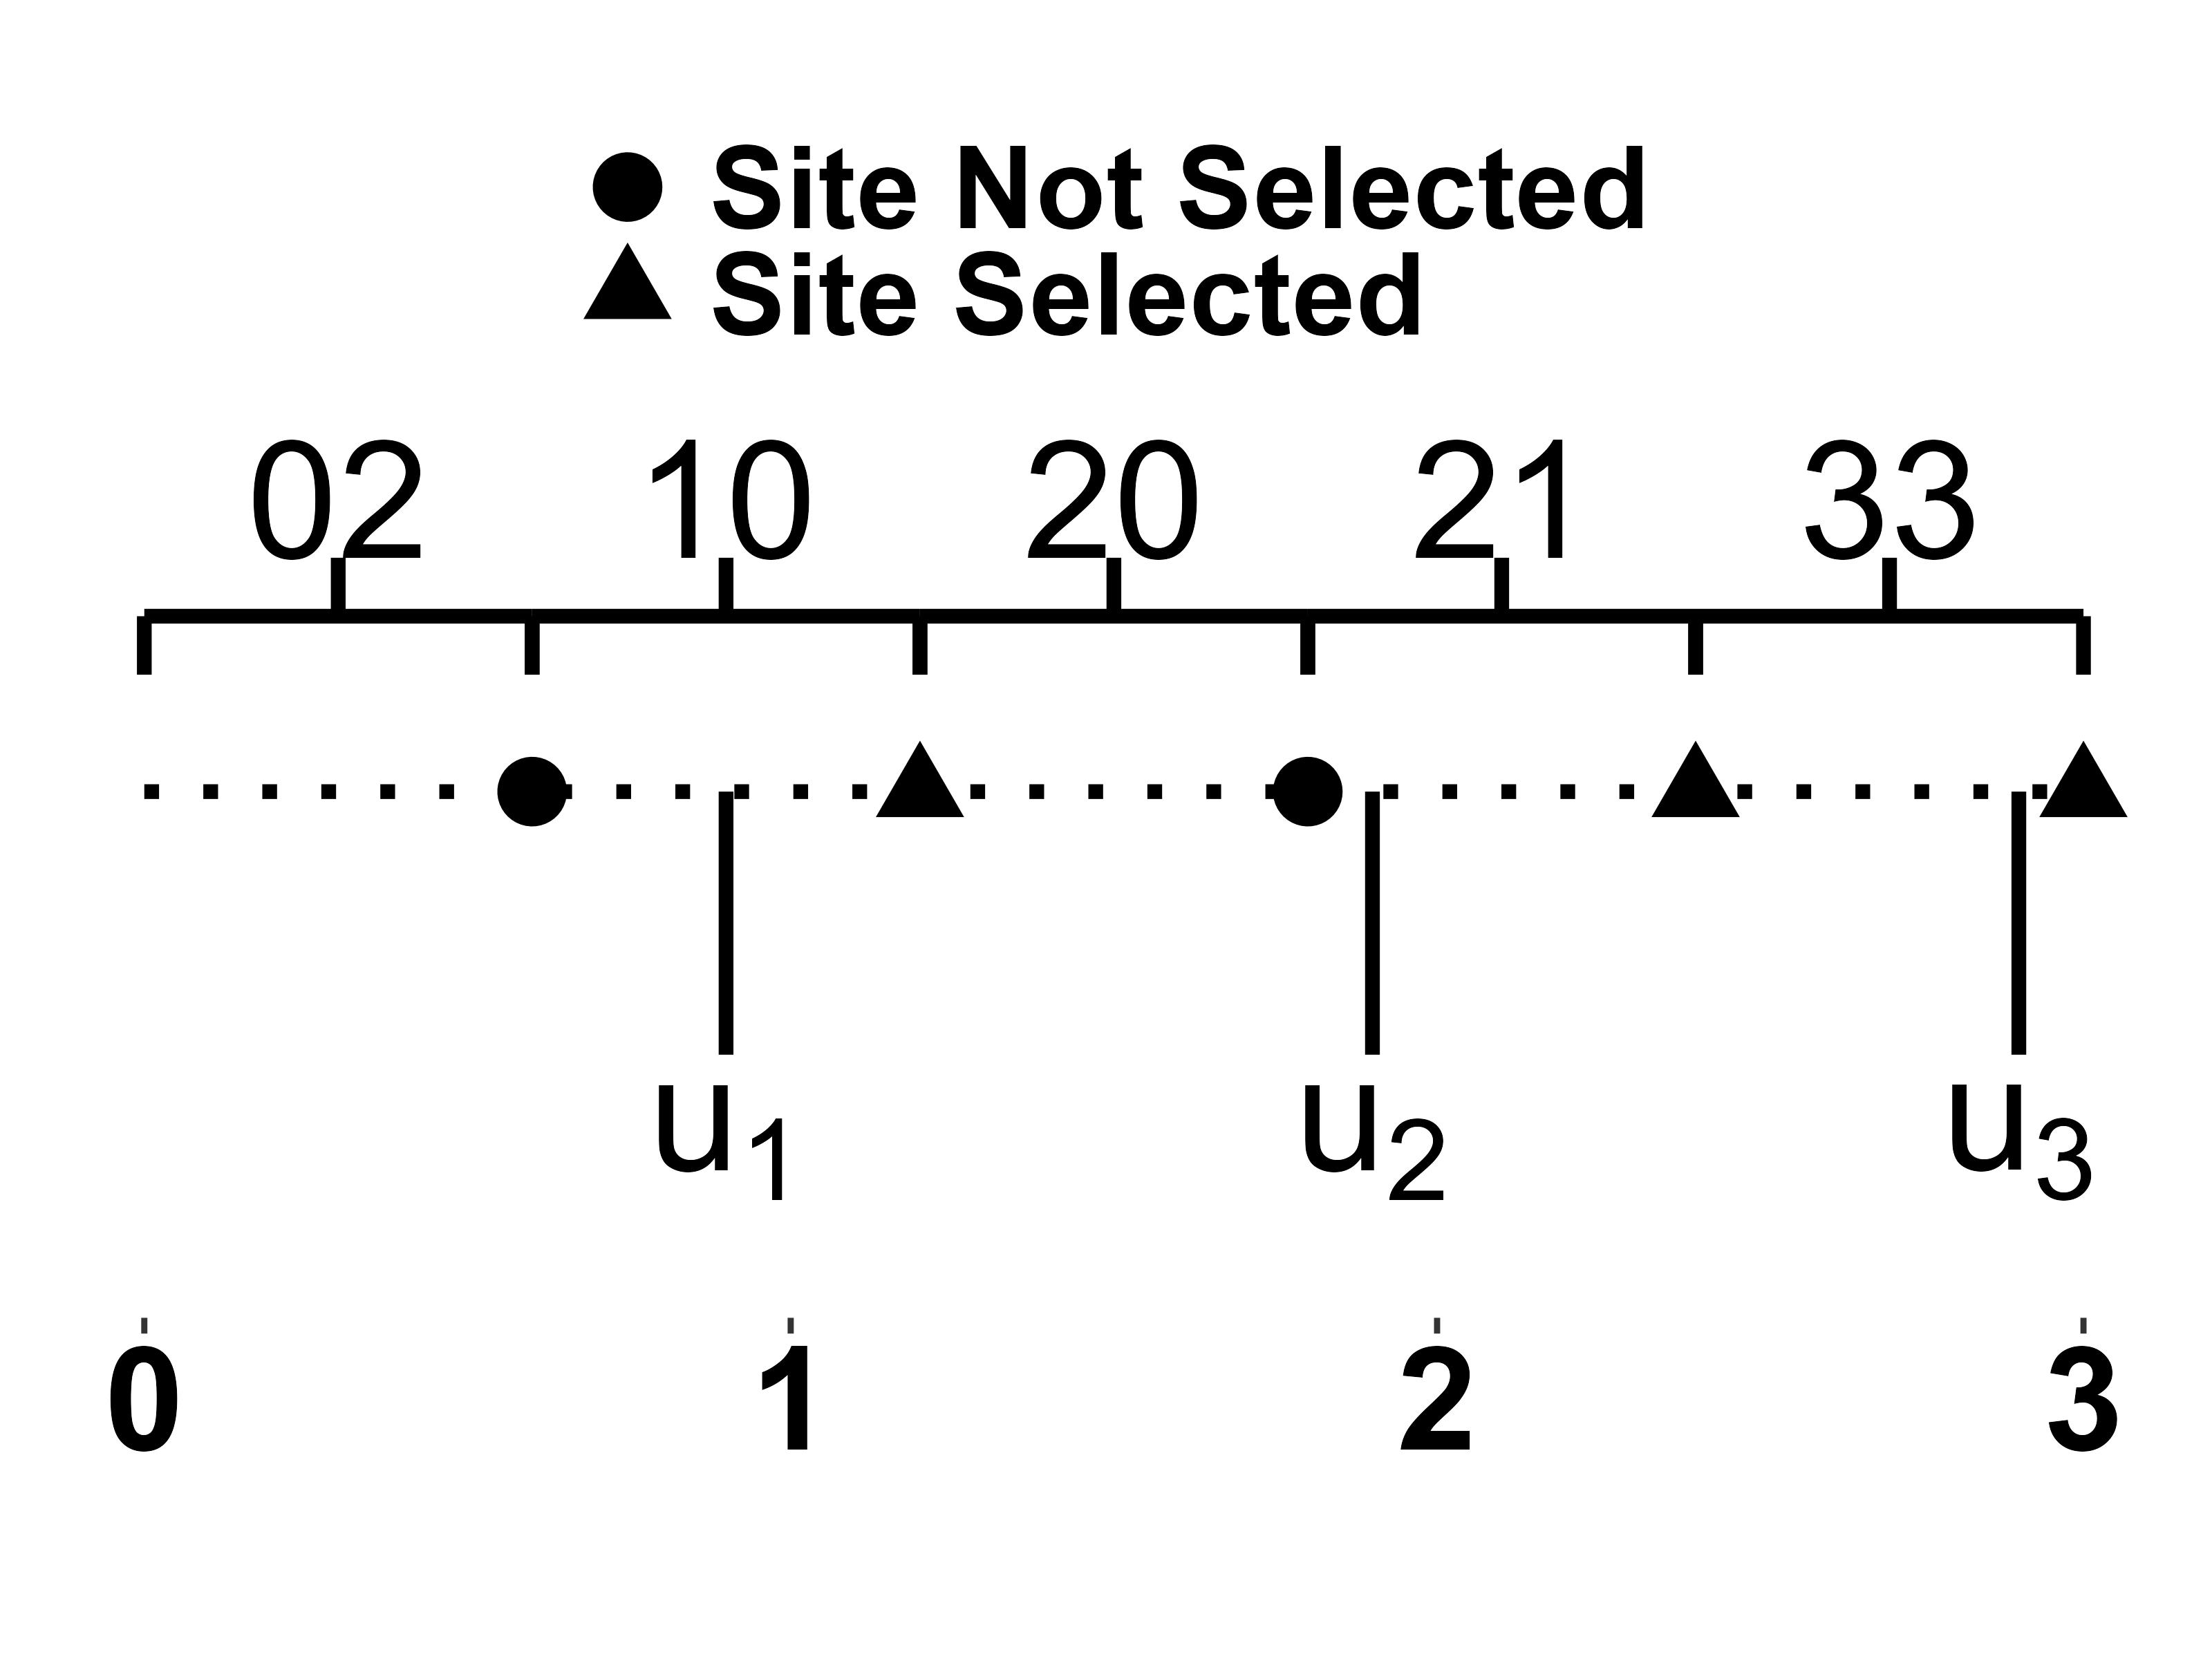
\includegraphics[width = 1\linewidth]{images/grts_line.jpeg}
  \caption{}
  \label{fig:grts_line}
\end{subfigure}
\begin{subfigure}{0.45\textwidth}
  \centering
  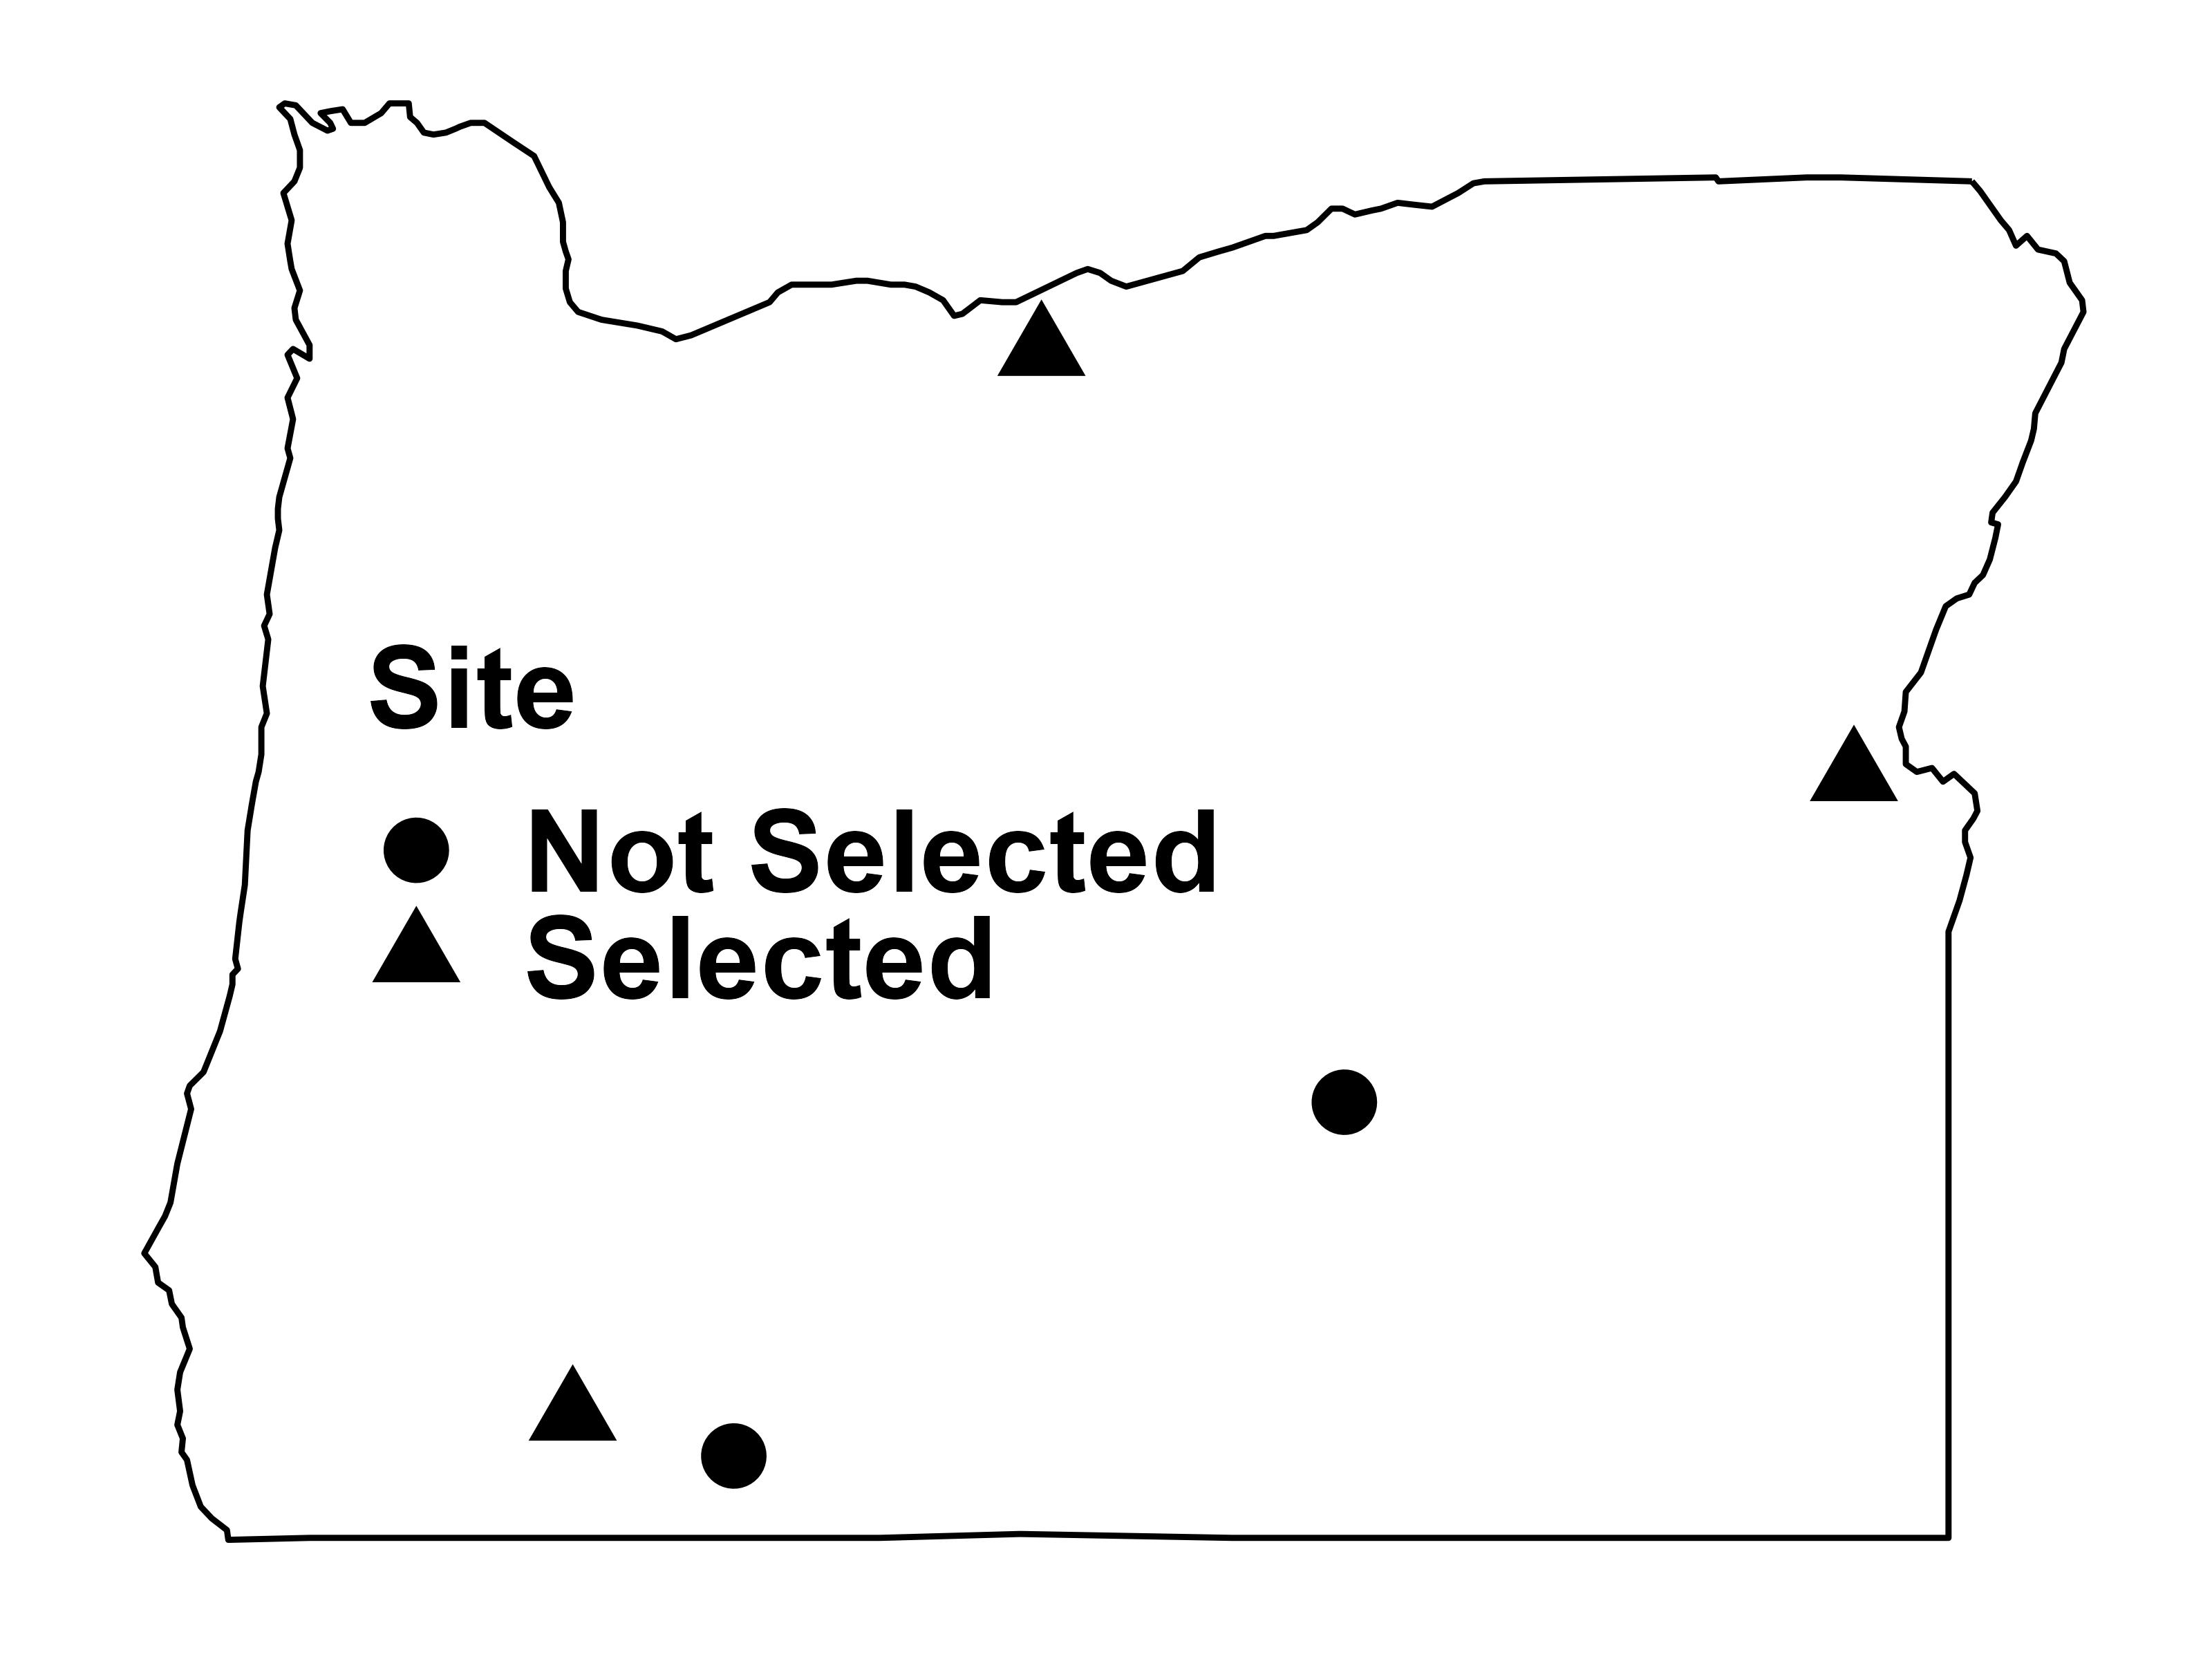
\includegraphics[width = 1\linewidth]{images/grts_sample.jpeg}
  \caption{}
  \label{fig:grts_sample}
\end{subfigure}
\caption{A visual description of the generalized random-tessellation stratified algorithm using sites from an illustrative sampling frame in Oregon, USA. In (a), the level-one cells are superimposed onto the sampling frame. In (b), the level-two cells are superimposed onto the sampling frame. In (c), the level-two cells are mapped in heirarchical order from two-dimensional space to a line and a sample is selected. Each cell is represented by brackets with a closed right endpoint, meaning they contain the site at their closed right boundary. In (d), the sites are separated by whether or not they are part of the sample.}
\label{fig:comps}
\end{figure}

Next the elements in \(\mathcal{A}_k\) are placed in hierarchical order.
Hierarchical order is a numeric order that first sorts \(\mathcal{A}_k\)
by the level-one addresses from smallest to largest, then by the
level-two addresses from smallest to largest, and so on. For example,
\(\mathcal{A}_2\) in hierarchical order is the set
\(\{00, 01, 02, 03, 10, ..., 13, 20, ..., 23, 30, ..., 33\}\). Then the
level-\(k\) grid cells are mapped from two-dimensional space to a line
in hierarchical order (Figure\(~\)\ref{fig:grts_line}). More
specifically, mapping a level-\(k\) grid cell means placing each site in
the level-\(k\) grid cell on the line, where each site is represented by
a line segment with length equal to its inclusion probability. The
hierarchical ordering tends to map nearby sites in two-dimensional space
to nearby locations on the line. Because the entire line represents the
inclusion probabilities of each site, the line's total length equals the
sum of these inclusion probabilities. This sum equals \(n\), the desired
sample size.

After hierarchically ordering the sites and placing them on the line,
the sample is selected. To select a sample, \citet{stevens2004grts}
denote a uniform random variable simulated from \([0, 1]\) as \(u_1\)
and place it on the line. The location of \(u_1\) on the line
corresponds falls within some line segment that represents a site, which
we denote \(s_1\). The site \(s_1\) is then the first site selected as
part of the sample. Next we define \(u_2 \equiv u_1 + 1\), which falls
within a line segment that represents another site, which we denote
\(s_2\). The sites \(s_1\) and \(s_2\) must be distinct because of the
requirement that each level-\(k\) cell has inclusion value no greater
than one. Then \(u_3 \equiv u_2 + 1\) corresponds to \(s_3\) and so on
until the set \(\{u_1, ..., u_n\}\) corresponds to the set
\(\{s_1, ..., s_n\}\), which are the \(n\) sites included in the sample
(Figure\(~\)\ref{fig:grts_sample}). \citet{stevens2004grts} provide
further details.

\pkg{spsurvey} implements the GRTS algorithm using the \code{grts()}
function. There are two required arguments to \code{grts()}: the
sampling frame and a base sample size. The first required argument is
the sampling frame, which must be an \pkg{sf} object. For point
resources, the \pkg{sf} geometries must all be \code{POINT} or
\code{MULTIPOINT}; for linear resources, the \pkg{sf} geometries must
all be \code{LINESTRING} or \code{MULTILINESTRING}; and for areal
resources, the \pkg{sf} geometries must all be \code{POLYGON} or
\code{MULTIPOLYGON}. The second required argument is the desired sample
size for the base sample, \code{n_base}. The base sample is a sample
that does not include replacement sites
(Section\(~\)\ref{subsubsec:repl_sites}). Additional arguments to the
\code{grts()} function address specific sampling design options, which
we discuss later.

The output from the \code{grts()} function is a list five components:
\code{sites_legacy}, \code{sites_base}, \code{sites_over},
\code{sites_near}, and \code{design}. \code{sites_legacy},
\code{sites_base}, \code{sites_over}, \code{sites_near} are \pkg{sf}
objects containing the legacy sites (discussed in
Section\(~\)\ref{subsubsec:legacy}), base sites (except for those
already included in \code{sites_legacy}), replacement sites using
reverse hierarchical ordering (Section\(~\)\ref{subsubsec:repl_sites}),
and replacement sites using nearest neighbor
(Section\(~\)\ref{subsubsec:repl_sites}), respectively. Together, the
collection of these \code{sites} objects are called the design sites.
Each \code{sites} objects contains all original columns from the
sampling frame and some additional columns related to the sampling
design. The last component of the \code{grts()} function output is a
list named \code{design}, which contains details regarding the sampling
design. Next we give some examples implementing the \code{grts()}
function.

To select a GRTS sample of size 50 where each site has an equal
inclusion probability, run

\begin{CodeChunk}
\begin{CodeInput}
R> eqprob <- grts(NE_Lakes, n_base = 50)
\end{CodeInput}
\end{CodeChunk}

Instead of sampling from the entire sampling frame simultaneously, it is
common to divide a sampling frame into distinct sets of sites known as
strata and select samples from each stratum independently of other
strata. This approach is known as stratification and yields a stratified
sample. \citet{sarndal2003model} mentions several practical and
statistical benefits of stratified samples compared to unstratified
samples. One such practical benefit is that stratification allows for
stratum-specific sample sizes and implementation practices (e.g., each
stratum may have different sampling protocols). One such statistical
benefit is that stratification tends to increase precision of parameter
estimates. To select a GRTS sample stratified by the lake elevation
categories where all sites within a stratum have equal inclusion
probabilities, run

\begin{CodeChunk}
\begin{CodeInput}
R> n_strata <- c(low = 35, high = 15)
R> eqprob_strat <- grts(
+   NE_Lakes,
+   n_base = n_strata,
+   stratum_var = "ELEV_CAT"
+ )
\end{CodeInput}
\end{CodeChunk}

In a stratified sample, \code{n_base} must be a named vector whose names
(low and high) represent each stratum and whose values represent
stratum-specific sample sizes (35 and 15). \code{stratum_var} is the
name of the column in the sampling frame that represents the
stratification variable.

Sometimes the desire is to sample sites that belong to some level of a
categorical variable more often than others levels. For example, suppose
large lakes are to be sampled more often than small lakes. To select a
GRTS sample with unequal inclusion probabilities based on lake area
categories, run

\begin{CodeChunk}
\begin{CodeInput}
R> caty_n <- c(small = 10, large = 40)
R> uneqprob <- grts(
+   NE_Lakes,
+   n_base = 50,
+   caty_n = caty_n,
+   caty_var = "AREA_CAT"
+ )
\end{CodeInput}
\end{CodeChunk}

\code{caty_n} is a named vector whose names represent the categorical
area levels (small and large) and whose values represent the expected
within-level sample sizes. \code{caty_var} is the name of the column in
the sampling frame that represents the unequal probability variable. If
the sample is stratified, \code{caty_n} must instead be a list whose
names match the names of \code{n_base} and whose values are named
vectors. Each named vector has names that represent the categorical
variable levels and values that represent within-strata expected sample
sizes.

Another approach is to sample sites proportionally to a positive
auxiliary variable, which is sometimes referred to as proportional to
size (PPS) sampling. PPS sampling can yield more efficient estimators
when the response and auxiliary variables are positively correlated
\citet{sarndal2003model}. To select a GRTS sample with inclusion
probabilities proportional to lake area, run

\begin{CodeChunk}
\begin{CodeInput}
R> propprob <- grts(
+   NE_Lakes,
+   n_base = 50,
+   aux_var = "AREA"
+ )
\end{CodeInput}
\end{CodeChunk}

\code{aux_var} is the name of the column in the sampling frame that
represents the PPS auxiliary variable.

\hypertarget{subsubsec:legacy}{%
\subsubsection{Legacy sites}\label{subsubsec:legacy}}

Often it is desired that some sites selected from an old sample are
guaranteed to be selected in a new sample. \citet{foster2017spatially}
discusses two types of sites that can be used to accomplish this goal:
legacy (historical) sites and iconic sites. Legacy sites were randomly
selected in the old sample, are in the current sampling frame, and must
be in the current sample. Together, this implies that the new sample can
be viewed as a possible joint realization from solely the current
sampling frame. Legacy sites are often used to study behavior through
time and can beneficial to estimation \citet{urquhart1999designs}.
Iconic sites, however, are not required to be randomly selected in the
old sample or to be contained in the current sampling frame. Iconic
sites are typically used because they represent sites of particular
importance -- consider a lake with a historically high level of a
dangerous chemical. Because iconic sites are not selected randomly, they
are not useful for estimation using the design-based approach.

Suppose the goal is to select a base GRTS sample of size \(n\) that
includes \(n_l\) legacy sites. The GRTS algorithm requires a small
adjustment to incorporate these legacy sites. Legacy sites are first
assigned inclusion probabilities as if they were non-legacy sites. Then
the level-\(k\) grid cells are hierarchically ordered and mapped to the
line (which has length \(n\)). The line lengths for the legacy sites are
then increased to one. The line lengths of the remaining sites are
scaled by \((n - n_l) /(n - \sum_i \pi_{i, l})\), where \(\pi_{i, l}\)
is the original line length of the \(i\)th legacy site. This scaling
ensures the total line length remains \(n\). The sample can then
selected using the \(u_i\) from Section\(~\)\ref{subsec:grts_algorithm}.
Because the legacy sites have line length one, they will always be
selected as the \(u_i\) are systematically spaced by one. This scaling
is only used to select the sample -- the design weights for data
analysis (discussed in Section\(~\)\ref{sec:analysis}) are based on the
pre-scaled inclusion probabilities.

The \code{grts()} function accommodates legacy sites using the
\code{legacy_sites} argument. \linebreak \code{legacy_sites} is an
\pkg{sf} object that contains the legacy sites as \code{POINT} or
\code{MULTIPOINT} geometries and uses the same coordinate reference
system as the sampling frame. The \linebreak \code{NE_Lakes_Legacy} data
in \pkg{spsurvey} contains five legacy sites. To select a sample of size
50 that includes the legacy sites and gives non-legacy sites an equal
inclusion probability, run

\begin{CodeChunk}
\begin{CodeInput}
R> eqprob_legacy <- grts(
+   NE_Lakes,
+   n_base = 50,
+   legacy_sites = NE_Lakes_Legacy
+ )
\end{CodeInput}
\end{CodeChunk}

When accommodating legacy sites, \code{n_base} (50) equals the sum of
the legacy sites (5) and the number of desired non-legacy sites (45). If
the sampling design uses stratification, unequal selection
probabilities, or proportional selection probabilities, the names of the
columns representing these variables in \code{legacy_sites} must be
provided using the \code{legacy_stratum_var}, \code{legacy_caty_var}, or
\code{legacy_aux_var} arguments, respectively. By default, \linebreak
\code{legacy_stratum_var}, \code{legacy_caty_var}, and
\code{legacy_aux_var} are assumed to have the same name as
\code{stratum_var}, \code{caty_var}, and \code{aux_var}, respectively.

\hypertarget{subsubsec:mindis}{%
\subsubsection{A minimum distance between
sites}\label{subsubsec:mindis}}

Recall that the GRTS algorithm selects sites that are spatially balanced
with respect to the sampling frame, not geography. Because of this, the
GRTS algorithm may select sites that are closer together in space than a
practitioner desires. The GRTS algorithm can sacrifice some spatial
balance with respect to the sampling frame to incorporate a minimum
distance requirement between sites selected in a sample:

\begin{CodeChunk}
\begin{CodeInput}
R> min_d <- grts(NE_Lakes, n_base = 50, mindis = 1600)
\end{CodeInput}
\end{CodeChunk}

The units of \code{mindis} must match the units of the sampling frame
for the minimum distance requirement to be applied properly. The
technical details for the GRTS algorithm's minimum distance adjustment
are omitted here, but they involve an iterative component that is
controlled by the \code{maxtry} argument to the \code{grts()} function.
If the minimum distance requirement cannot be met for all sites selected
in the sample, a warning message is returned. If the sample is
stratified, \code{mindis} can be a list with stratum-specific minimum
distance requirements.

\hypertarget{subsubsec:repl_sites}{%
\subsubsection{Replacement sites}\label{subsubsec:repl_sites}}

Sometimes a site is selected in the sample but data are not able to be
collected at the site. This commonly occurs due to landowner denial or a
lack of funding, among other reasons. When this occurs, it is helpful to
have a set of replacement sites so that the desired sample size can
still be reached. The \code{grts()} function provides two options for
replacement sites: reverse hierarchical ordering and nearest neighbor.

\citet{stevens2004grts} proposed the reverse hierarchical approach for
selecting replacement sites. Suppose the desired number of base sites is
\(n\) and replacement sites is \(n_r\). The GRTS algorithm is first used
to select a spatially balanced sample of size \(n + n_r\). Recall that
part of the GRTS algorithm is placing the sites in hierarchical order
according to the set
\(\{a_1...a_k : a_1 = 0, 1, 2, 3; ...; a_k = 0, 1, 2, 3\}\). Simply
selecting the first \(n - n_r\) hierarchically ordered sites to be in
the base sample is insufficient because nearby sites have nearby
hierarchical addresses. Instead, the reverse hierarchical approach
reverses the hierarchical address of the \(n + n_r\) sites, yielding a
new ordering according to the set
\(\{a_k...a_1 : a_k = 0, 1, 2, 3; ...; a_1 = 0, 1, 2, 3\}\). Then the
first \(n - n_r\) reverse hierarchically ordered sites compose the base
sample and the remaining \(n_r\) are the replacement sites. If a base
site cannot be evaluated, the first of the \(n_r\) replacement sites is
used instead, and so on. This reverse hierarchical ordering ensures the
\(n - n_r\) base sites retain as much spatial balance as possible.
Because the GRTS sample is selected for a sample size of \(n + n_r\),
the larger that \(n_r\) is relative to \(n\), the less spatially
balanced the base sites, so choosing a realistic value for \(n_r\) is
important. To select a GRTS sample of size 50 with 10 reverse
hierarchically ordered replacement sites, run

\begin{CodeChunk}
\begin{CodeInput}
R> eqprob_rho <- grts(NE_Lakes, n_base = 50, n_over = 10)
\end{CodeInput}
\end{CodeChunk}

The value supplied to \code{n_base} is \(n\), and the value supplied to
\code{n_over} is \(n_r\). If the sample is stratified, \code{n_over} can
be a list with stratum-specific reverse hierarchical ordering
requirements.

An alternative approach for replacement sites is the nearest neighbor
approach. The nearest neighbor approach selects replacement sites after
a GRTS sample of size \(n\) is selected. For each site in the GRTS
sample, the distance is calculated between that site and all other sites
in the sampling frame that are not part of the GRTS sample. Then the
nearest \(n_n\) sites are selected as replacement sites. The replacement
sites are ordered from smallest distance to the largest distance; for
example, the first replacement site is the site closest to the base
site. To select a GRTS sample of size 50 with two nearest neighbor
replacement sites for each base site, run

\begin{CodeChunk}
\begin{CodeInput}
R> eqprob_nn <- grts(NE_Lakes, n_base = 50, n_near = 2)
\end{CodeInput}
\end{CodeChunk}

The value supplied to \code{n_base} is \(n\), and the value supplied to
\code{n_near} is \(n_n\). If the sample is stratified, \code{n_near} can
be a list with stratum-specific nearest neighbor requirements.

\hypertarget{sec:eda_samples}{%
\subsection{Summarizing, visualizing, and binding design
sites}\label{sec:eda_samples}}

The \code{summary()} and \code{plot()} functions in \pkg{spsurvey} are
also used to summarize and visualize the design sites (all the sites
contained in \code{sites_legacy}, \code{sites_base}, \code{sites_over},
and \code{sites_near}). \code{summary()} and \code{plot()} for design
sites require the object output from \code{grts()} and a formula. The
formula is used the same way as it is for \code{summary()} and
\code{plot()} applied to sampling frames, though using \code{summary()}
and \code{plot()} for design sites requires the formula contains
\code{siteuse}. \code{siteuse} is a categorical variables added to
\code{sites_legacy}, \code{sites_base}, \code{sites_over}, and
\code{sites_near} that indicates the site type (\code{Legacy},
\code{Base}, \code{Over}, or \code{Near}). Incorporating \code{siteuse}
enables breaking up the summaries and visualizations by site type. The
default formula when summarizing or visualizing design sites is
\code{~ siteuse}.

Recall \code{eqprob_rho} is the unstratified, equal probability GRTS
sample with reverse hierarchically ordered replacement sites. To
visualize the design sites for \code{eqprob_rho}
(Figure\(~\)\ref{fig:base_over}), run

\begin{CodeChunk}
\begin{CodeInput}
R> plot(eqprob_rho)
\end{CodeInput}
\end{CodeChunk}

By default, \code{plot()} will use all non-\code{NULL} \code{sites}
objects. To request particular \code{sites} objects, use the
\code{siteuse} argument (Figure\(~\)\ref{fig:base}):

\begin{CodeChunk}
\begin{CodeInput}
R> plot(eqprob_rho, siteuse = "Base")
\end{CodeInput}
\end{CodeChunk}

\begin{figure}
\centering
\begin{subfigure}{0.49\textwidth}
  \centering
  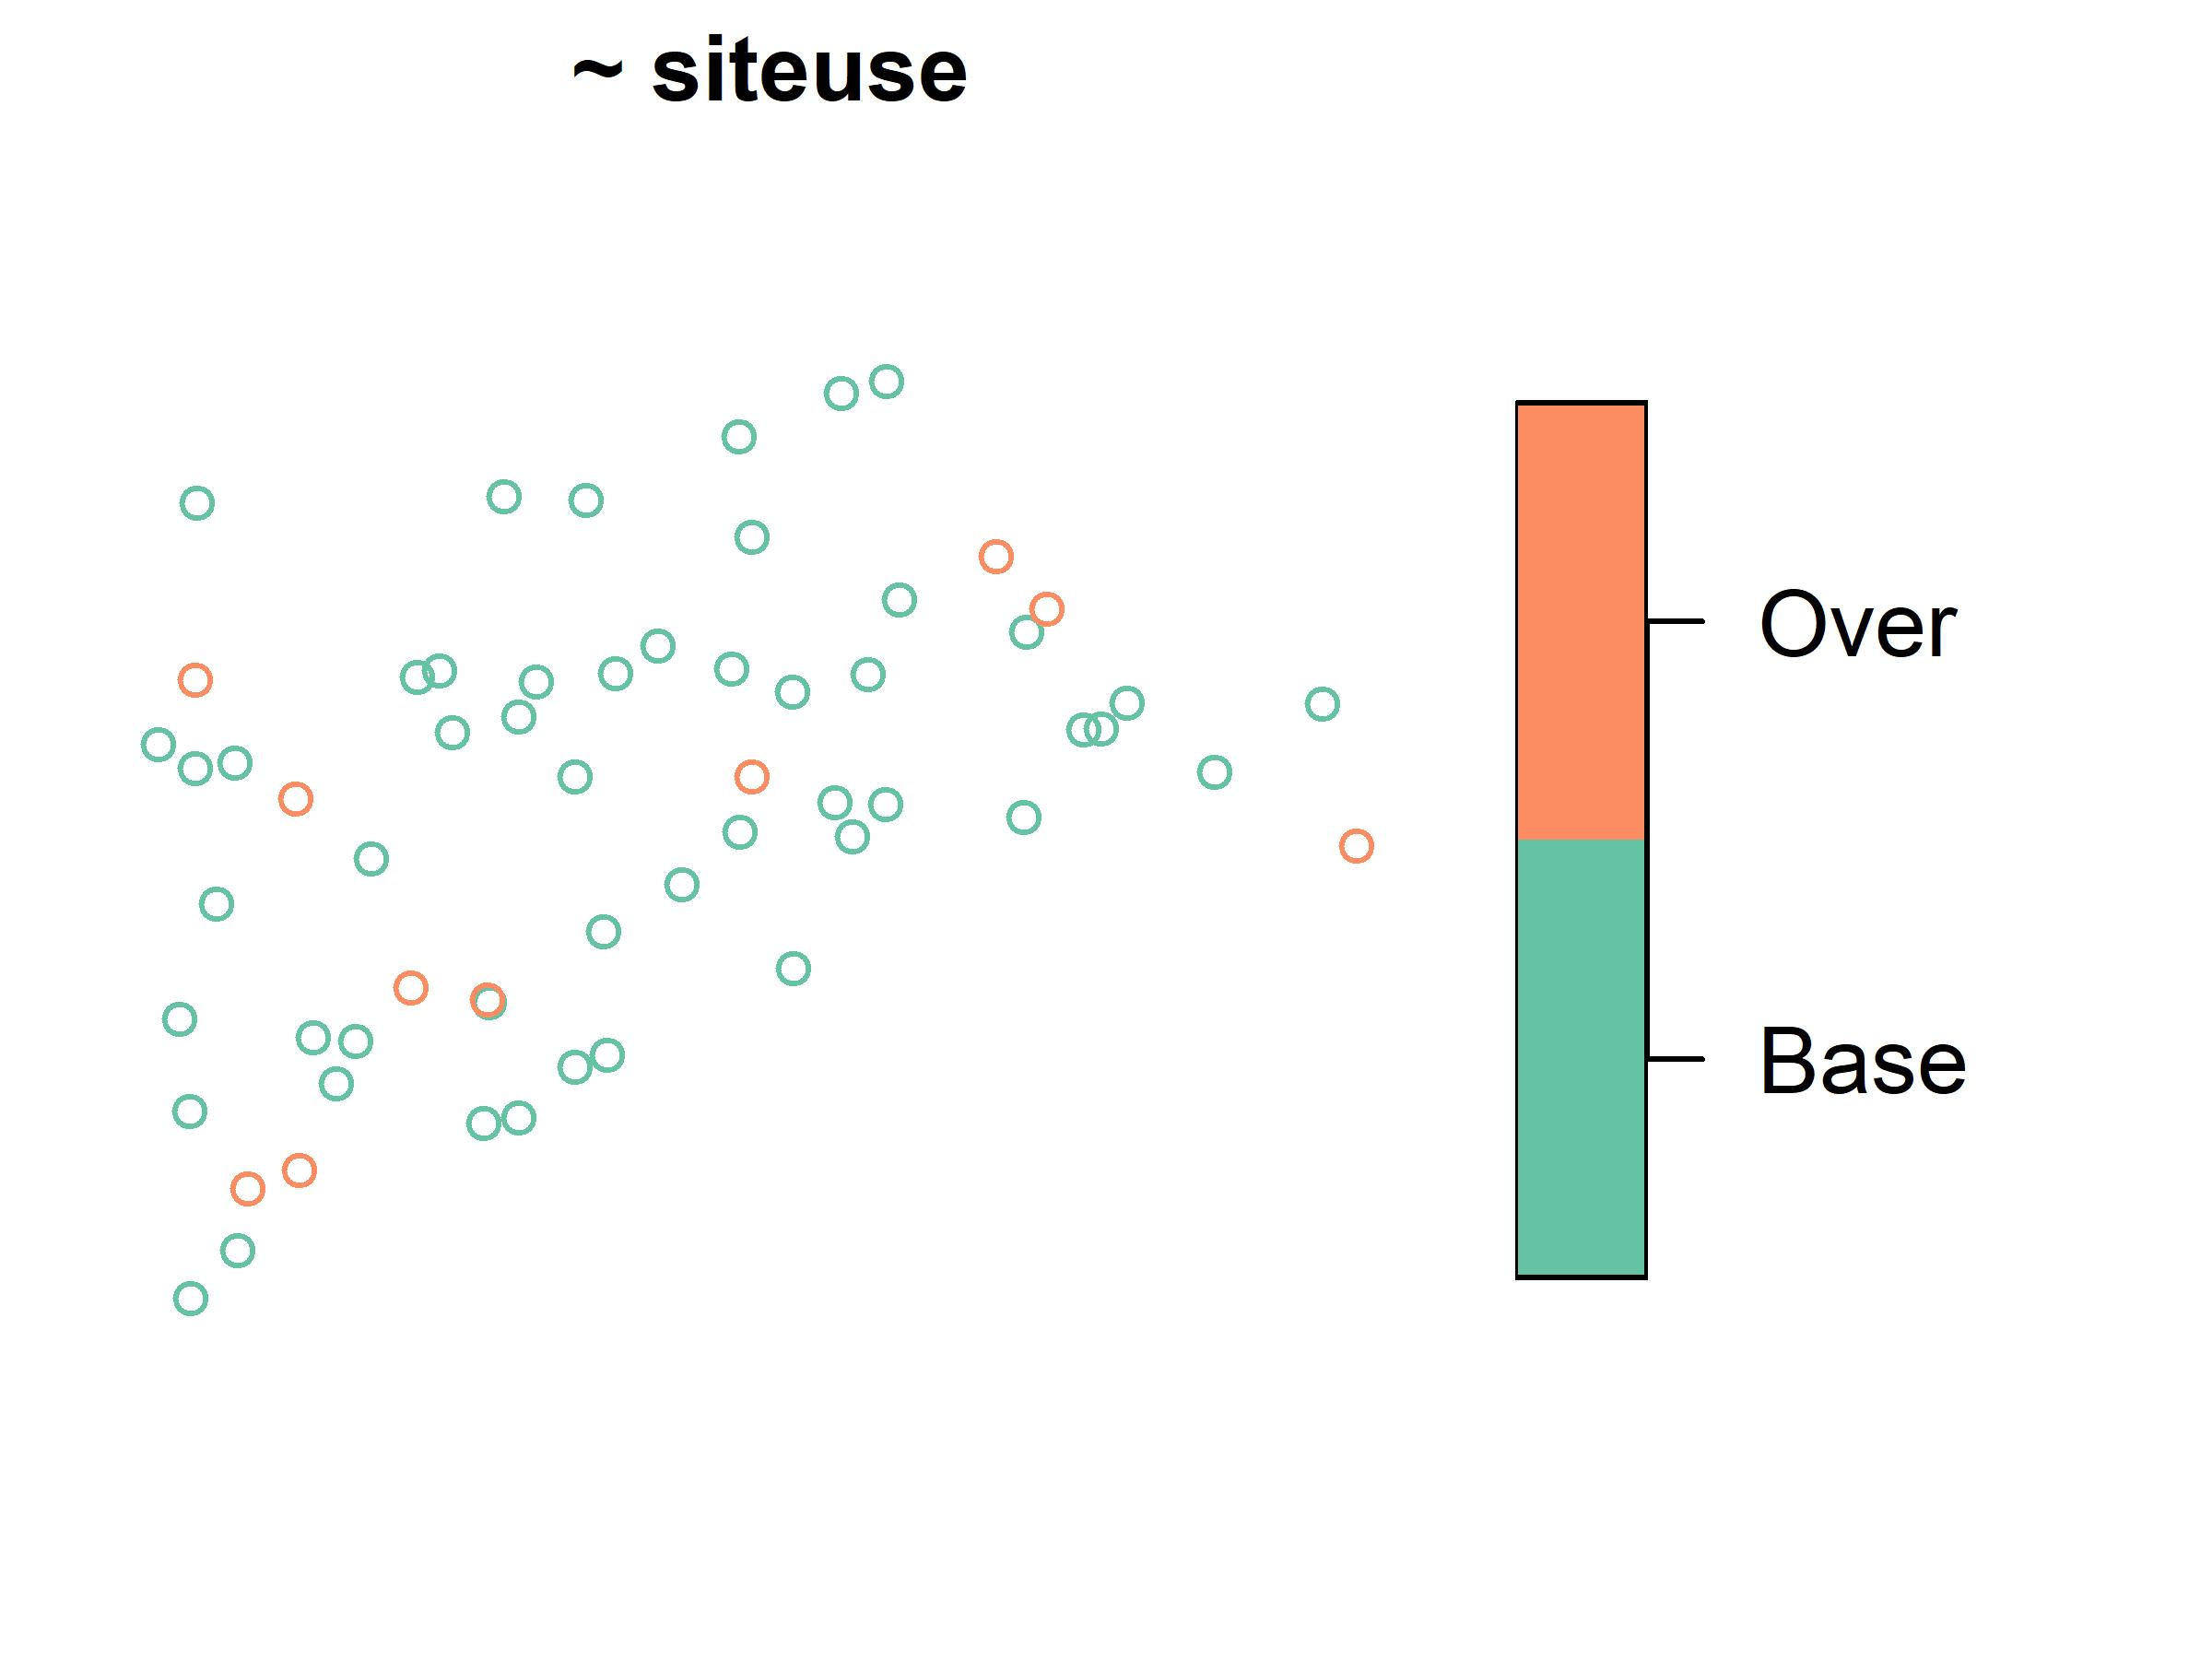
\includegraphics[width = 1\linewidth]{images/base_over.jpeg}
  \caption{}
  \label{fig:base_over}
\end{subfigure}
\begin{subfigure}{0.49\textwidth}
  \centering
  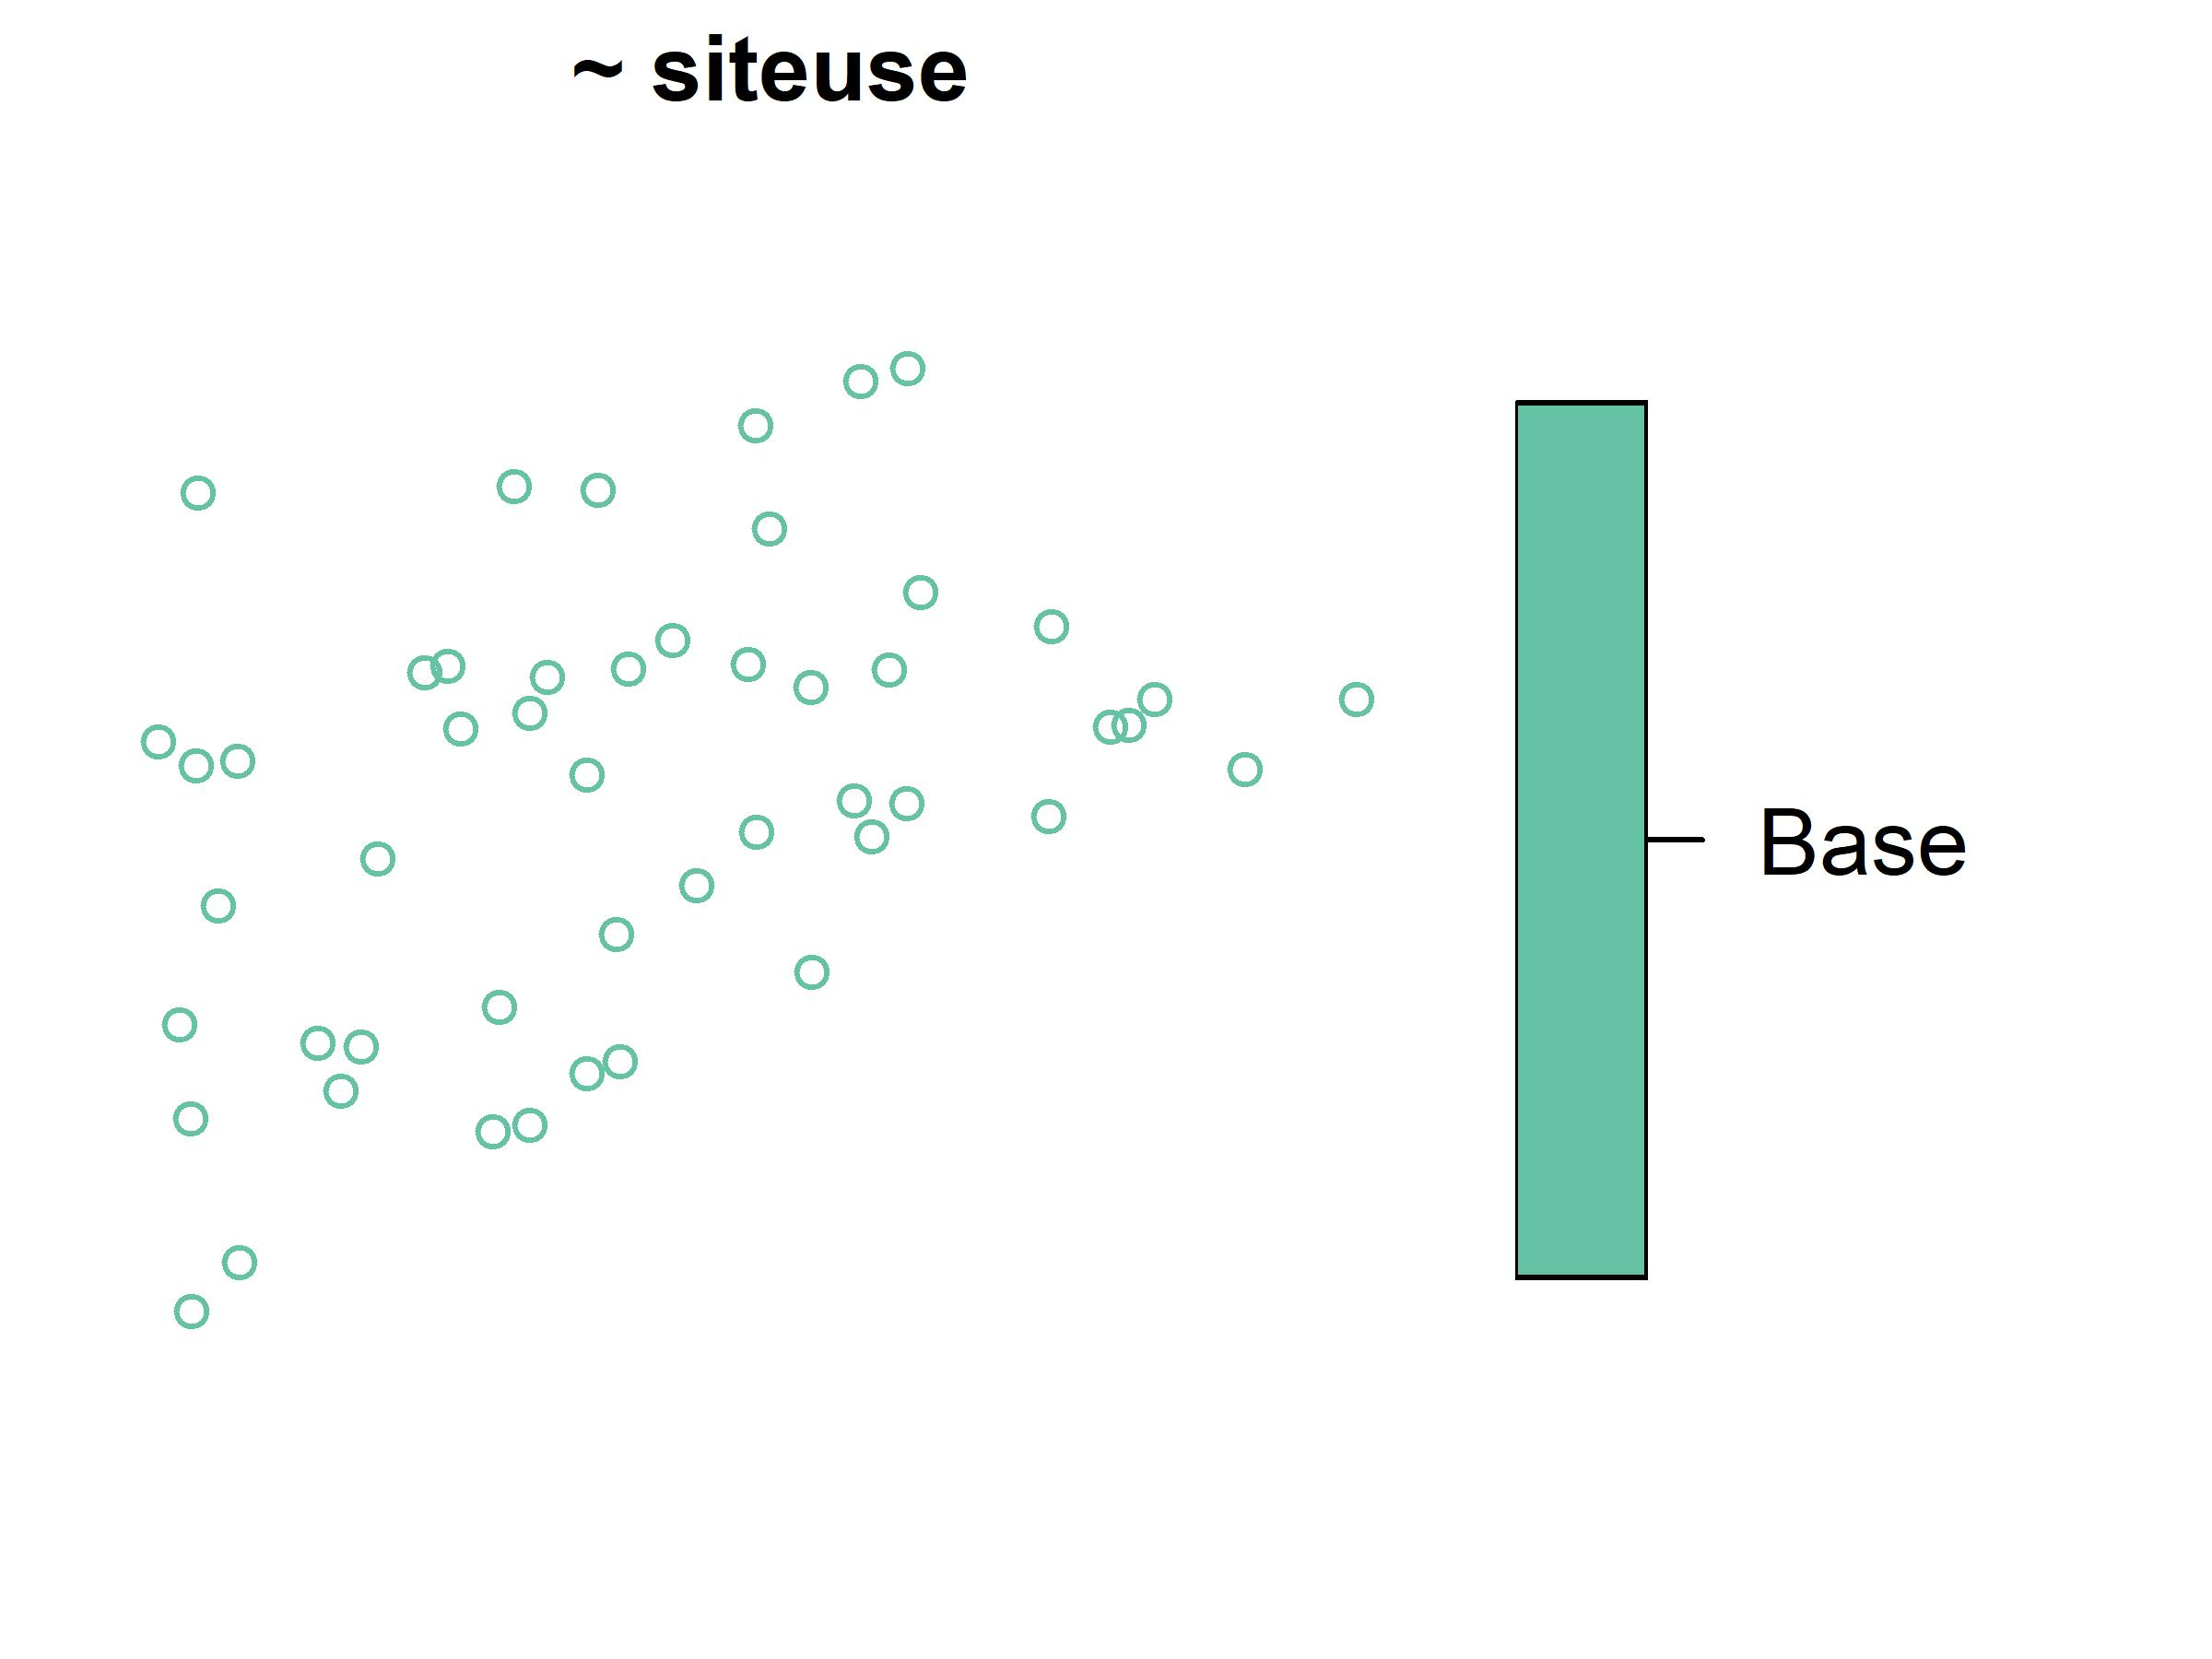
\includegraphics[width = 1\linewidth]{images/base.jpeg}
  \caption{}
  \label{fig:base}
\end{subfigure} 
\caption{Base and replacement (using reverse hierarchical ordering) sites are shown for an unstratified, equal probability GRTS sample of the Northeastern lakes data. In (a), the base and replacement sites are shown. In (b), only the base sites are shown.}
\label{fig:base_and_over}
\end{figure}

The design sites can be overlain onto the sampling frame via the
\code{sframe} argument.

To summarize the design sites for each lake elevation level, run

\begin{CodeChunk}
\begin{CodeInput}
R> summary(eqprob_rho, formula = siteuse ~ ELEV_CAT)
\end{CodeInput}
\begin{CodeOutput}
siteuse by total: 
      Base Over
total   50   10

siteuse by ELEV_CAT: 
     Base Over
low    30    5
high   20    5
\end{CodeOutput}
\end{CodeChunk}

Running

\begin{CodeChunk}
\begin{CodeInput}
R> plot(eqprob_rho, formula = siteuse ~ ELEV_CAT)
\end{CodeInput}
\end{CodeChunk}

produces two separate visualizations: one for each level of
\code{ELEV_CAT}. To summarize lake area for each site type, run

\begin{CodeChunk}
\begin{CodeInput}
R> summary(eqprob_rho, formula = AREA ~ siteuse)
\end{CodeInput}
\begin{CodeOutput}
AREA by total: 
          Min.  1st Qu.   Median     Mean  3rd Qu.     Max.
total 1.043181 2.491625 3.833015 13.26145 7.540559 137.8127

AREA by siteuse: 
         Min.  1st Qu.   Median     Mean   3rd Qu.      Max.
Base 1.043181 2.539218 4.273565 14.52684 11.178641 137.81268
Over 1.767196 2.456281 2.804252  6.93449  5.619522  38.26573
\end{CodeOutput}
\end{CodeChunk}

Running

\begin{CodeChunk}
\begin{CodeInput}
R> plot(eqprob_rho, formula = AREA ~ siteuse)
\end{CodeInput}
\end{CodeChunk}

produces two separate visualizations: one for the \code{Base} sites and
another for the \code{Over} sites.

To bind together \code{sites_legacy}, \code{sites_base},
\code{sites_over}, and \code{sites_near} (four separate \pkg{sf}
objects) into a single \pkg{sf} object, use \code{sp_rbind()}:

\begin{CodeChunk}
\begin{CodeInput}
R> sites_bind <- sp_rbind(eqprob_rho)
\end{CodeInput}
\end{CodeChunk}

Then \code{sites_bind} is then easily written out using a function like
\code{sf::write_sf()}.

\hypertarget{sec:print}{%
\subsection{Printing design sites}\label{sec:print}}

Basic summaries of site counts in a design can be easily returned using
\code{print()}. These summaries represent the crossing of variable type
(total, stratification, unequal probability, and stratification and
unequal probability) with site type (\code{Legacy}, \code{Base},
\code{Over}, and \code{Near}). Only crossings used in the design are
returned. Next we print a design stratified by lake elevation category
with legacy sites, reverse hierarchically ordered replacement sites, and
nearest neighbor replacement sites

\begin{CodeChunk}
\begin{CodeInput}
R> n_strata <- c(low = 10, high = 10)
R> n_over_strata <- c(low = 2, high = 5)
R> print(grts(
+   NE_Lakes,
+   n_base = n_strata,
+   stratum_var = "ELEV_CAT",
+   legacy_sites = NE_Lakes_Legacy,
+   n_over = n_over_strata,
+   n_near = 1
+ ))
\end{CodeInput}
\begin{CodeOutput}
Summary of Site Counts: 

siteuse by total: 
      Legacy Base Over Near
total      5   15    7   27

siteuse by stratum: 
     Legacy Base Over Near
high      0   10    5   15
low       5    5    2   12
\end{CodeOutput}
\end{CodeChunk}

\hypertarget{sec:spb}{%
\subsection{Measuring spatial balance}\label{sec:spb}}

We have discussed the notion spatial balance but have not yet given a
way to measure it. \citet{stevens2004grts} proposed measuring spatial
balance using Voronoi polygons (i.e., Dirichlet Tessellations). A
Voronoi polygon for a base design site \(s_i\) contains the region in
the sampling frame closer to \(s_i\) than any other design site.
\citet{stevens2004grts} define \(v_i\) as the sum of the inclusion
probabilities for all sites in the sampling frame contained in the
\(i\)th Voronoi polygon. They show that the expected value of \(v_i\) is
1 for all \(i\). This framework motivates the use of loss metrics based
on Voronoi polygons to measure spatial balance. One loss metric is
Pielou's evenness index (PEI)
\citep{shannon1948mathematical, pielou1966measurement}, which is defined
as \begin{align}\label{eq:rmse}
  \text{PEI} = 1 +  \sum_{i = 1}^n \frac{v_i}{n} \ln(v_i / n) / \ln(n),
\end{align} where \(n\) is the sample size. PEI is bounded between zero
and one. A PEI of zero indicates perfect spatial balance. As PEI
increases, the spatial balance worsens.

The \code{sp_balance()} function in \pkg{spsurvey} measures spatial
balance and requires three arguments: a set of design sites, the
sampling frame, and a vector of loss metrics. The default loss metric is
\code{"pielou"} for PEI, though several other metrics are available. To
calculate PEI for the unstratified, equal probability GRTS sample with
no replacement sites (\code{eqprob}), run

\begin{CodeChunk}
\begin{CodeInput}
R> sp_balance(eqprob$sites_base, NE_Lakes) # grts
\end{CodeInput}
\begin{CodeOutput}
  stratum metric     value
1    None pielou 0.0301533
\end{CodeOutput}
\end{CodeChunk}

To highlight the benefit of the spatially balanced GRTS sampling, we can
select a simple random sample (SRS) using \pkg{spsurvey}'s \code{irs()}
function and measure its spatial balance (a SRS selects sites with equal
probability and independent of spatial location).

\begin{CodeChunk}
\begin{CodeInput}
R> eqprob_irs <- irs(NE_Lakes, n_base = 50)
R> sp_balance(eqprob_irs$sites_base, NE_Lakes) # srs
\end{CodeInput}
\end{CodeChunk}

\begin{CodeChunk}
\begin{CodeOutput}
  stratum metric      value
1    None pielou 0.04589258
\end{CodeOutput}
\end{CodeChunk}

The GRTS sample has better spatial balance than the SRS sample because
the PEI value is lower in the GRTS sample. For stratified samples,
spatial balance metrics can be calculated separately for each stratum
using the \code{stratum_var} argument. We explore the relationship
between spatial balance and estimation in
Section\(~\)\ref{sec:application}.

\hypertarget{linear-and-areal-sampling-frames}{%
\subsection{Linear and areal sampling
frames}\label{linear-and-areal-sampling-frames}}

The examples in Section\(~\)\ref{sec:design} have thus far been applied
to point resources. Applications to linear and areal resources use the
same syntax -- all that changes is the geometry type of the \code{sf}
object used as an argument. For example, we select an equal probability
GRTS sample of size 25 from \code{Illinois_River}, a linear resource of
reach segments on the \code{Illinois_River}, by running

\begin{CodeChunk}
\begin{CodeInput}
R> eqprob_linear <- grts(Illinois_River, n_base = 25)
\end{CodeInput}
\end{CodeChunk}

We visualize the sample overlain onto the sampling frame
(Figure\(~\)\ref{fig:grts_illinois}) by running

\begin{CodeChunk}
\begin{CodeInput}
R> plot(eqprob_linear, sframe = Illinois_River, pch = 19)
\end{CodeInput}
\end{CodeChunk}

Notice how the sample units area spread throughout the reach segments.
The same approach can be used to select GRTS sample of size 40 from
\code{Lake_Ontario}, an areal resource of shoreline segments surrounding
Lake Ontario, by running

\begin{CodeChunk}
\begin{CodeInput}
R> eqprob_areal <- grts(Lake_Ontario, n_base = 40)
\end{CodeInput}
\end{CodeChunk}

We visualize the sample overlain onto the sampling frame
(Figure\(~\)\ref{fig:grts_ontario}) by running

\begin{CodeChunk}
\begin{CodeInput}
R> plot(eqprob_areal, sframe = Lake_Ontario, pch = 19)
\end{CodeInput}
\end{CodeChunk}

\begin{figure}
\centering
\begin{subfigure}{0.49\textwidth}
  \centering
  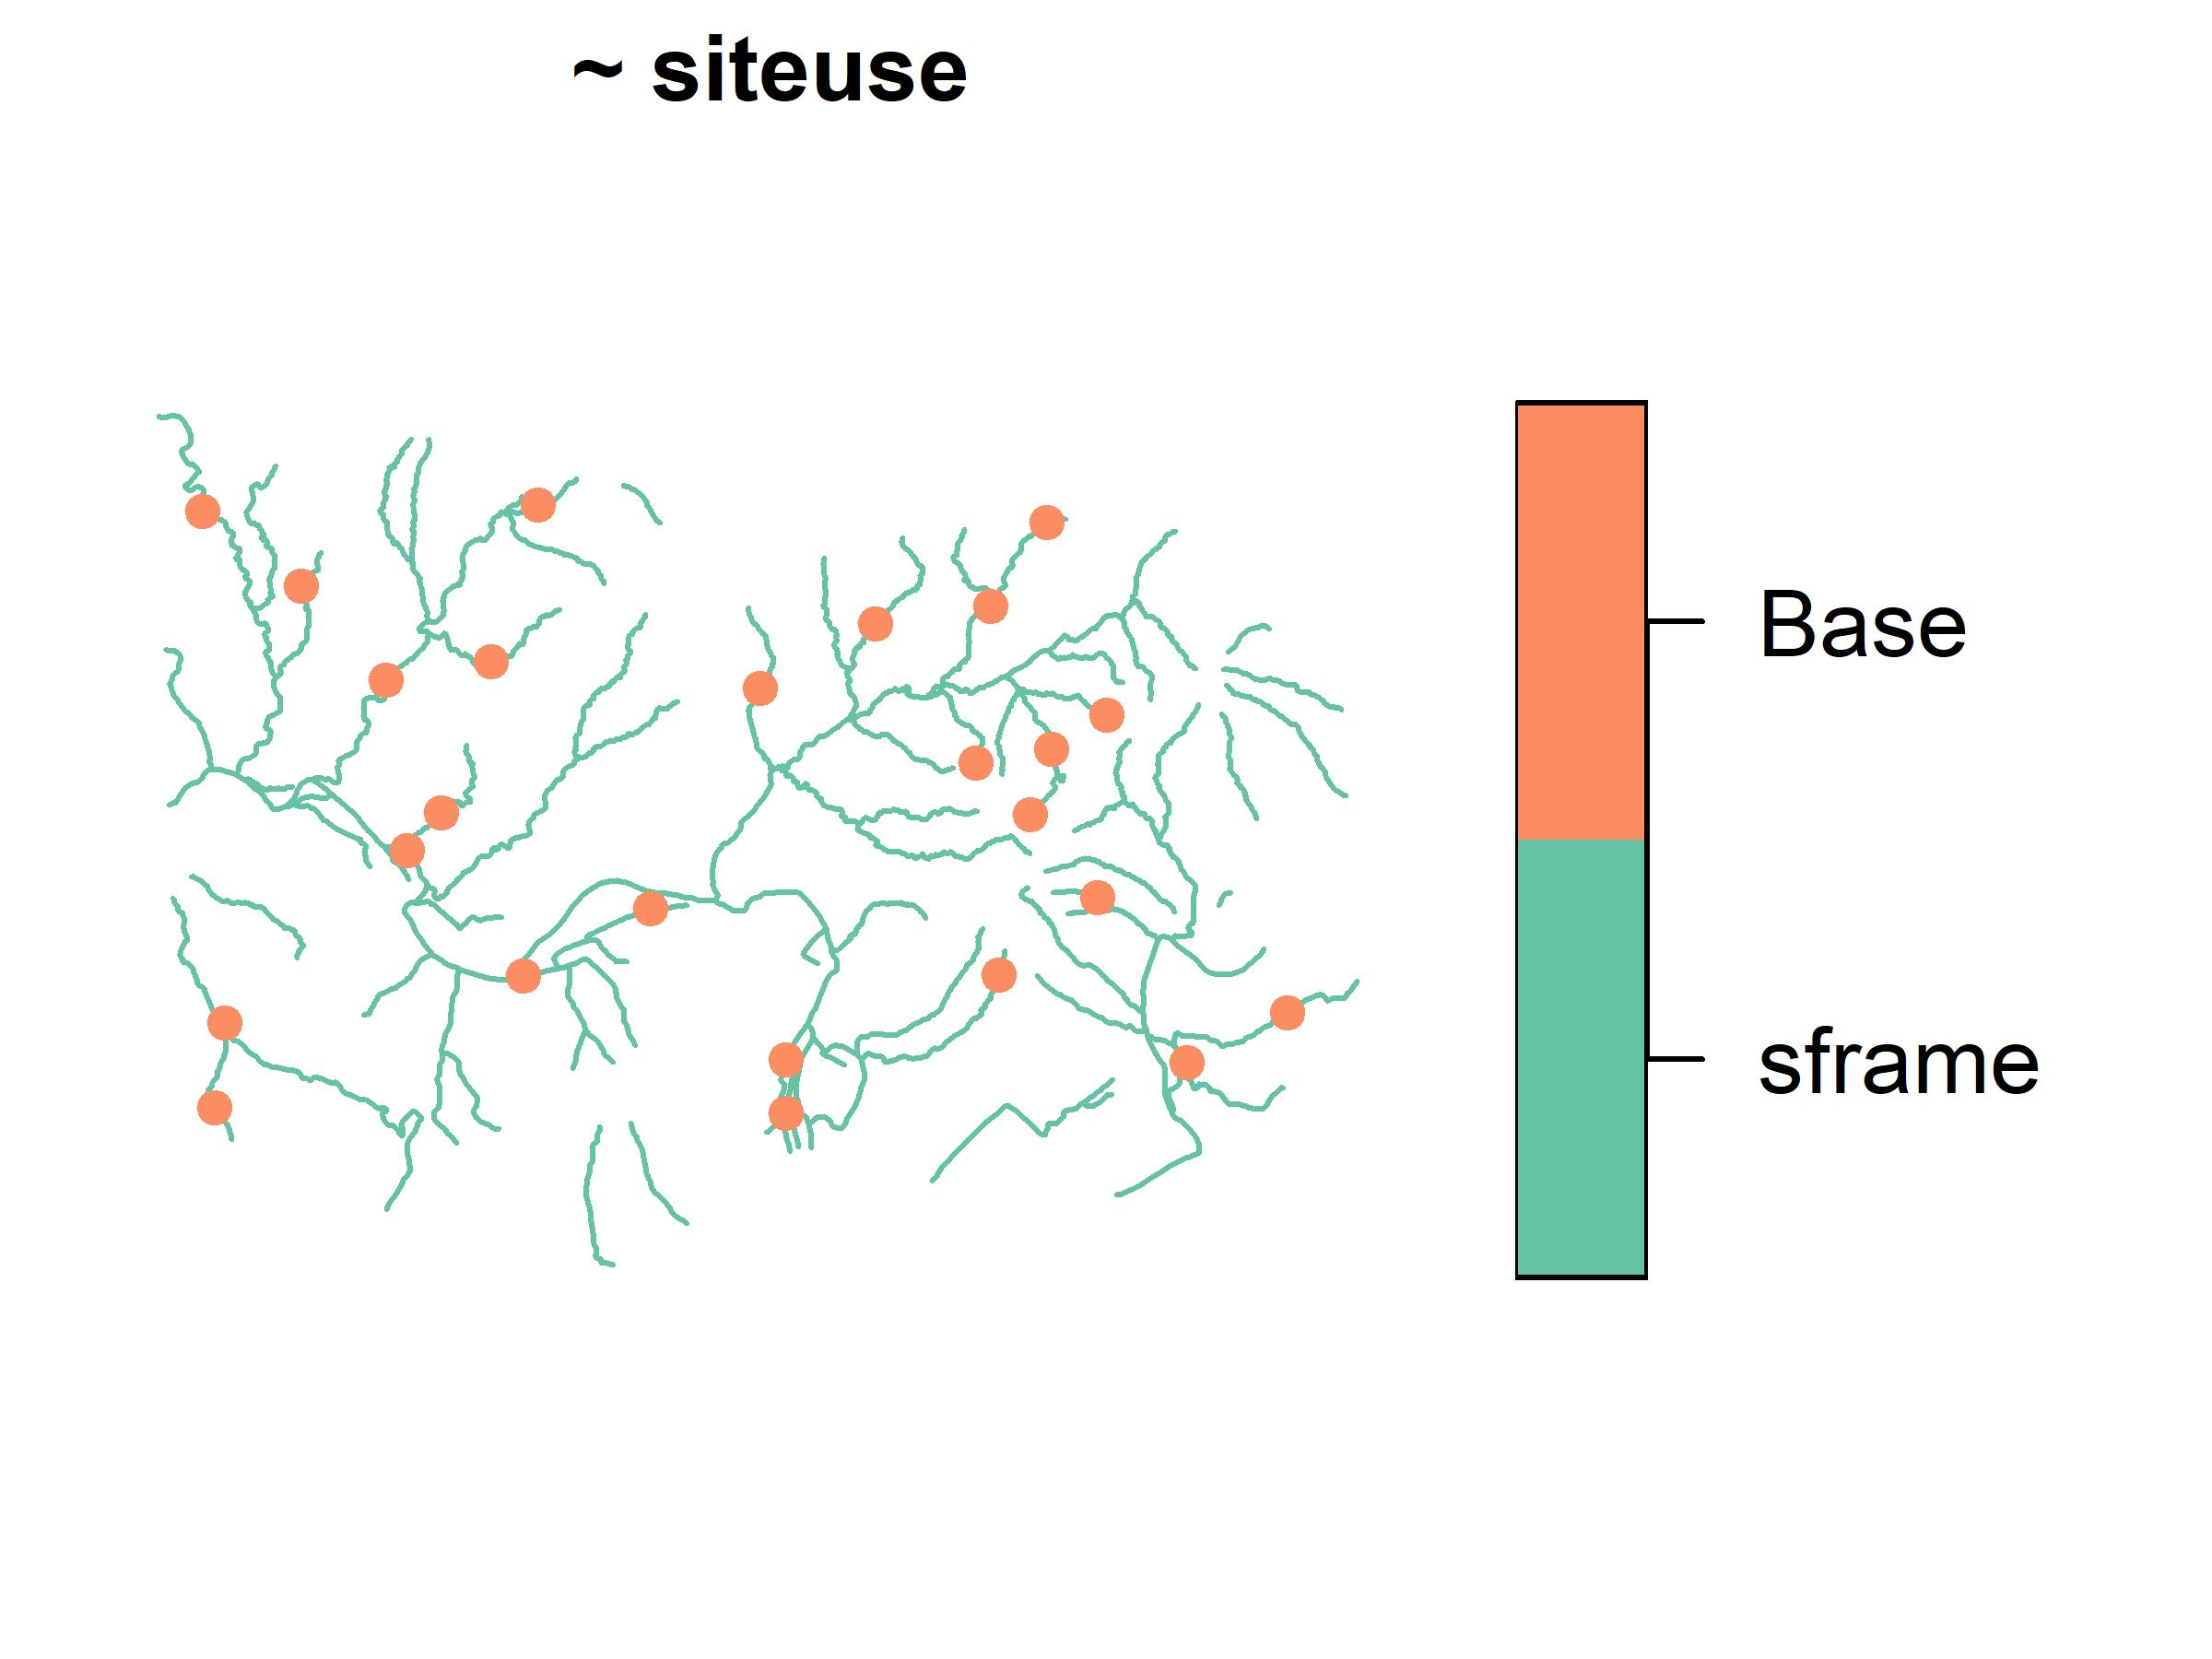
\includegraphics[width = 1\linewidth]{images/grts_illinois.jpeg}
  \caption{}
  \label{fig:grts_illinois}
\end{subfigure}
\begin{subfigure}{0.49\textwidth}
  \centering
  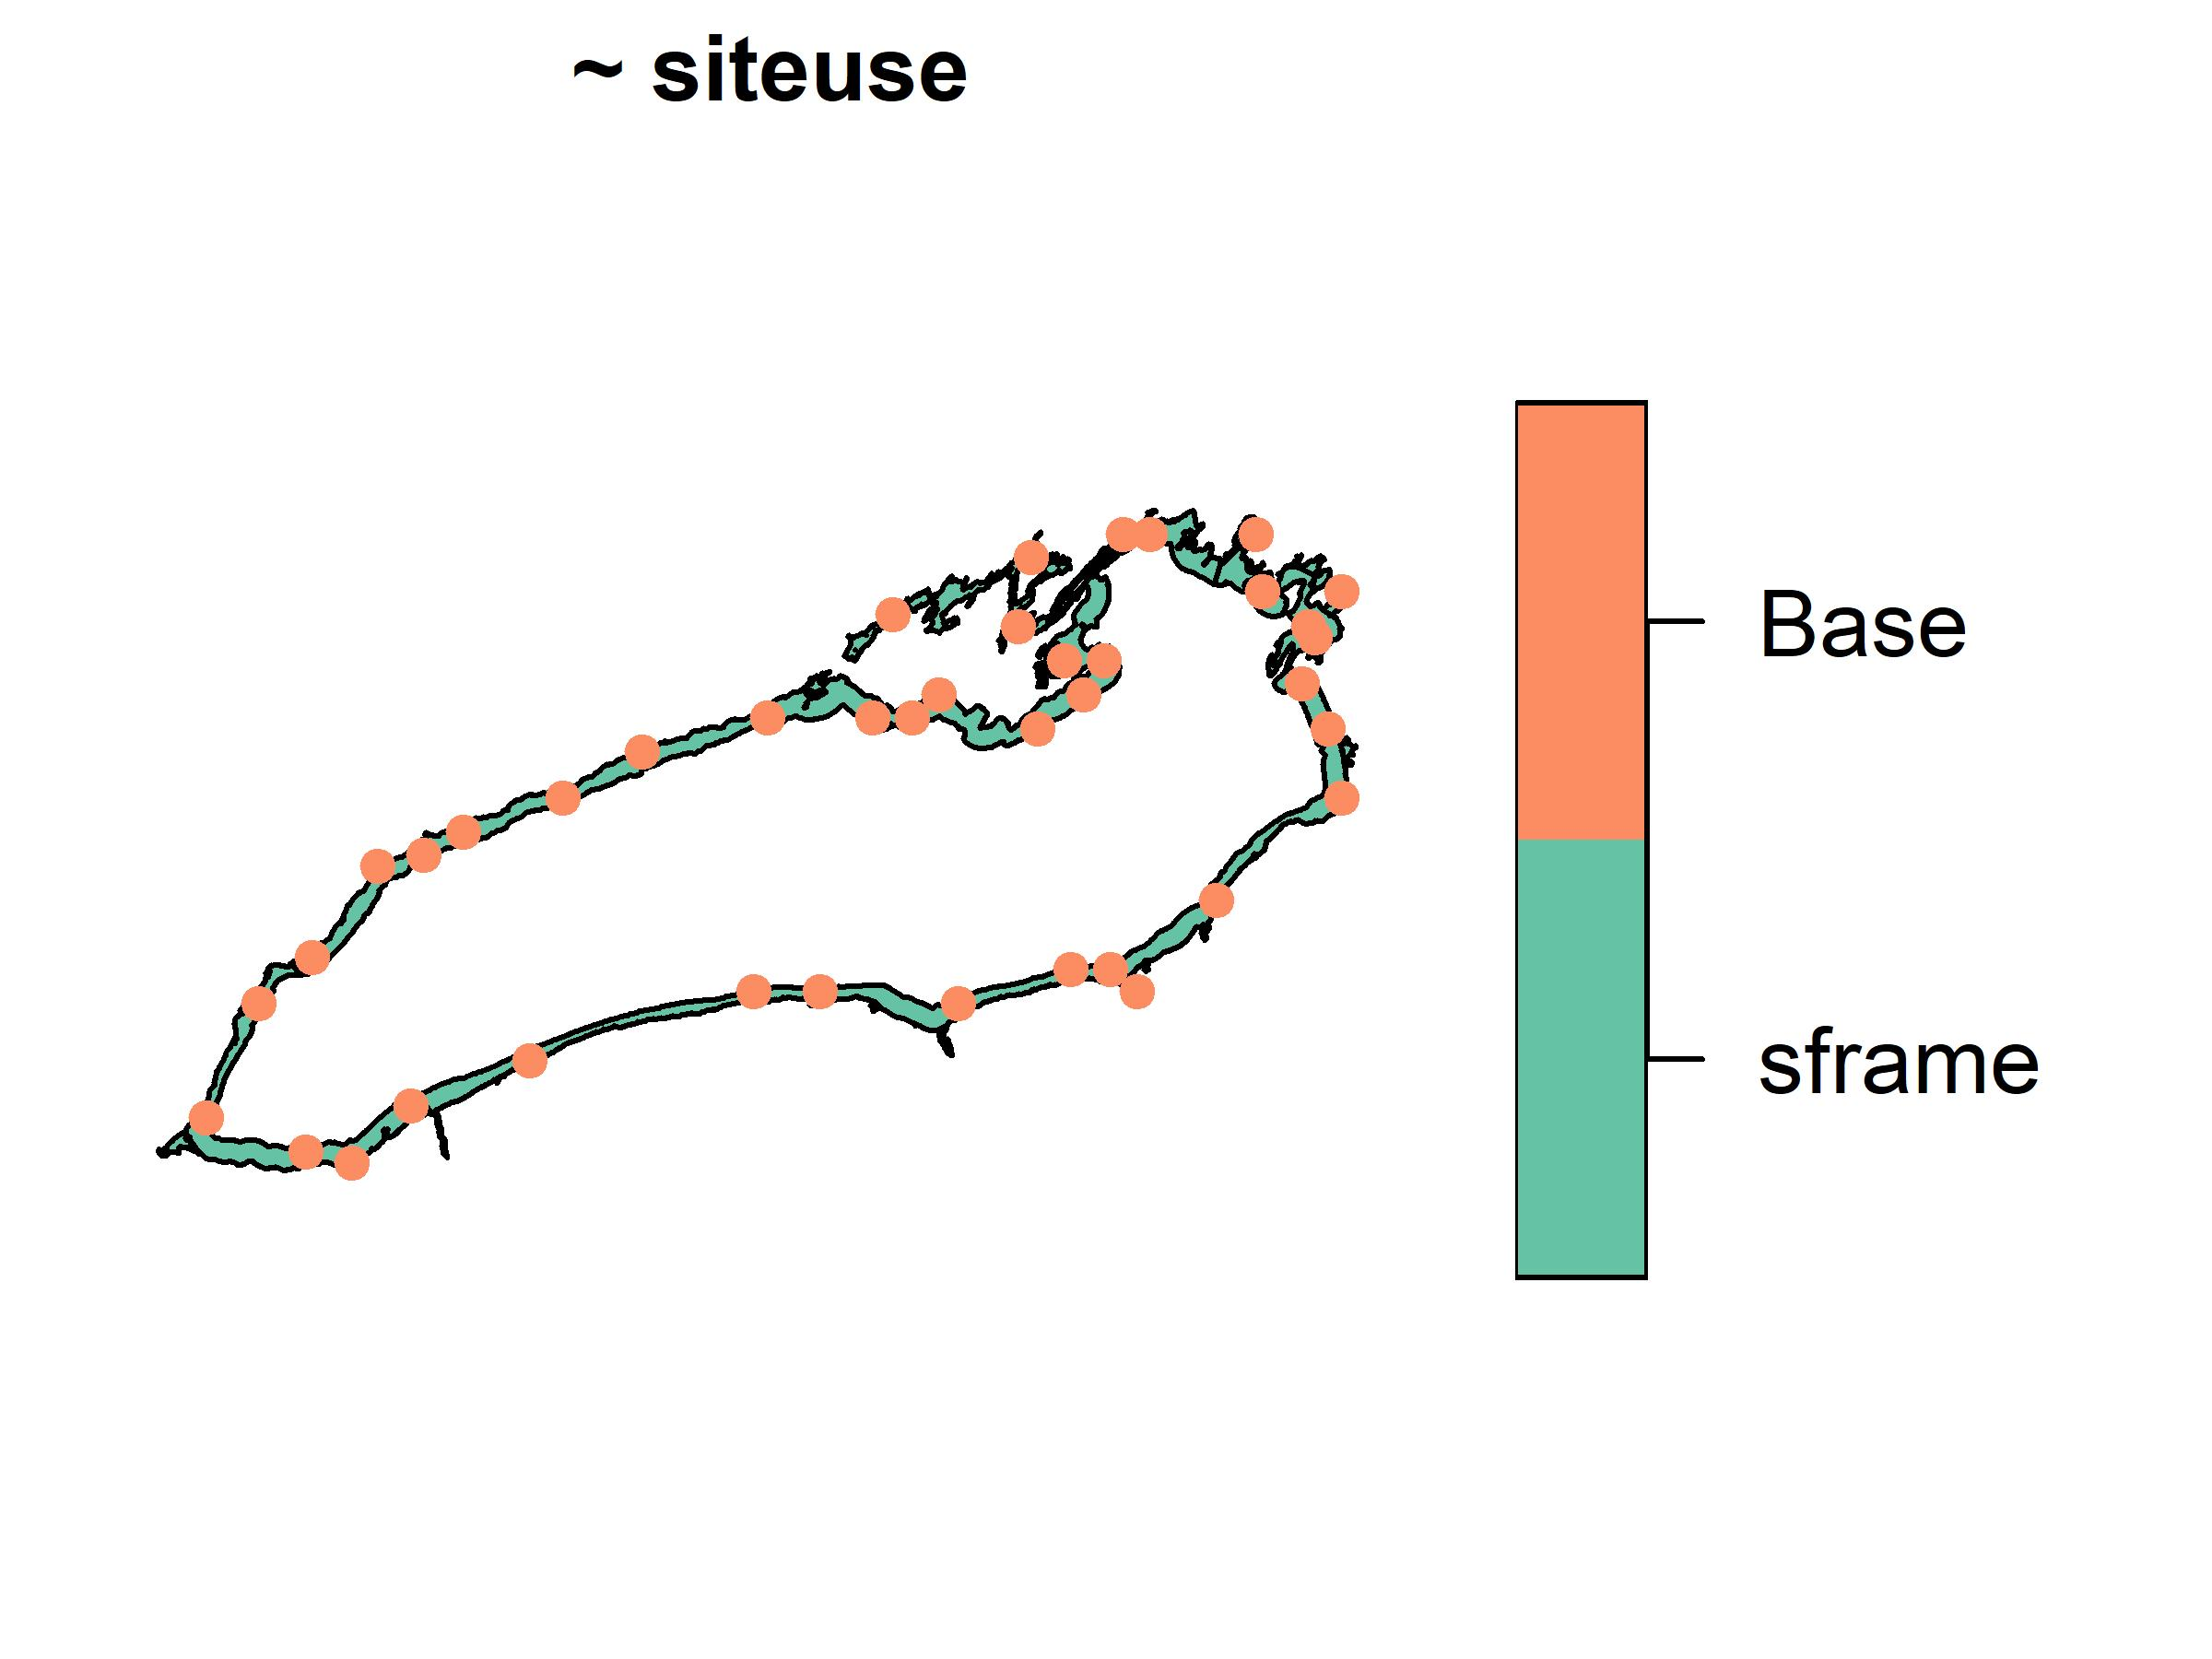
\includegraphics[width = 1\linewidth]{images/grts_ontario.jpeg}
  \caption{}
  \label{fig:grts_ontario}
\end{subfigure} 
\caption{Equal probability GRTS sample of size 20 from the Illinois River data (a) and the Lake Ontario data (b).}
\label{fig:lin_areal}
\end{figure}

Notice how the sample units are spread throughout the shoreline.

To learn more about how the GRTS algorithm accommodates each of the
three resource types (point, linear, areal), run \code{?grts} and view
the package vignettes (\code{vignette(package = "spsurvey")}. To learn
more about the \code{Illinois_River} and \code{Lake_Ontario} data in
\pkg{spsurvey}, run \code{?Illinois_River} and \code{Lake_Ontario},
respectively.

\hypertarget{sec:analysis}{%
\section{Analysis}\label{sec:analysis}}

After collecting data at the design sites, population parameters can be
estimated. Often times, these parameters are population proportions,
means, or totals. Suppose \(\tau\) represents a population total.
\citet{horvitz1952generalization} showed that an unbiased estimator of
\(\tau\) is given by \begin{align}\label{eq:horvthom}
  \hat{\tau} = \sum_{i = 1}^n \frac{y_i}{\pi_i},
\end{align} where \(n\) is the sample size, \(y_i\) is the response
variable measured at \(s_i\) (the \(i\)th design site), and \(\pi_i\) is
the inclusion probability of \(s_i\). The term \(\pi_i^{-1}\) is the
reciprocal of \(\pi_i\) and is called a design weight. The design weight
quantifies how many sites \(s_i\) represents in the sampling frame.
Though Equation\(~\)\ref{eq:horvthom} was originally derived for finite
populations, \citet{cordy1993extension} showed it remains unbiased for
infinite populations. Other parameters like proportions and means are
estimated using similar forms of Equation\(~\)\ref{eq:horvthom}.

\citet{horvitz1952generalization} showed that an unbiased estimator of
the variance of \(\hat{\tau}\) is given by
\begin{align}\label{eq:var_horvthom}
  \hat{\text{Var}}(\hat{\tau}) = \sum_{i = 1}^n \frac{(1 - \pi_i)}{\pi_i^2} y_i^2 + \sum_{i = 1}^n \sum_{i \neq j} \frac{(\pi_{ij} - \pi_i \pi_j)}{\pi_{ij} \pi_i \pi_j}y_i y_j ,
\end{align} where \(\pi_{ij}\) is the probability both \(s_i\) and
\(s_j\) are included in the sample. In a finite population simple random
sample, Equation\(~\)\ref{eq:var_horvthom} reduces to the following
well-known formula: \begin{align}\label{eq:var_irs}
  \hat{\text{Var}}(\hat{\tau}) = \frac{N(N - n)}{n(n - 1)}\sum_{i = 1}^n \left(y_i - \frac{\hat{\tau}}{N} \right)^2 ,
\end{align} where \(N\) equals the number of sites in the sampling
frame. \citet{sen1953estimate} and \citet{yates1953selection} derived a
similar unbiased estimator of the variance of \(\hat{\tau}\). Both this
estimator and Equation\(~\)\ref{eq:var_horvthom} rely on knowing the
\(\pi_{ij}\) for all \(s_i\) and \(s_j\). Calculating \(\pi_{ij}\) can
be very challenging for more complicated designs, so
\citet{hartley1962sampling}, \citet{overton1987sampling}, and
\citet{brewer2002combined} proposed different approaches to
approximating \(\pi_{ij}\) when estimating variances (as in
Equation\(~\)\ref{eq:var_horvthom}).

The aforementioned variance estimators and \(\pi_{ij}\) approximations
do not incorporate the spatial locations of the \(s_i\).
\citet{stevens2003variance} derived an estimator of the variance of
\(\tau\) that does incorporate the spatial locations of the \(s_i\) by
conditioning on random properties of the GRTS sample. This variance
estimator is called the local neighborhood variance estimator. The local
neighborhood variance estimator of \(\hat{\tau}\) is denoted
\(\hat{\text{Var}}(\hat{\tau})_{lnb}\) and is given by
\begin{align}\label{eq:var_lnb}
  \hat{\text{Var}}(\hat{\tau})_{lnb} = \sum_{i = 1}^n \sum_{s_j \in D(s_i)} w_{ij} \left(\frac{y_j}{\pi_j} - \sum_{s_k \in D(s_i)} w_{ik} \frac{y_k}{\pi_k} \right)^2 ,
\end{align} where the \(w_{ij}\) are weights and \(D(s_i)\) is the set
of design sites in \(s_i\)'s local neighborhood.
\citet{stevens2003variance} provide technical details and discuss how to
determine the local neighborhoods. Equation\(~\)\ref{eq:var_lnb} is
useful for two reasons. First, it does not rely on \(\pi_{ij}\). Second,
incorporating the spatial locations of the \(s_i\) tends to reduce the
variance of \(\hat{\tau}\) compared to a variance estimator that ignores
spatial locations, which leads to narrower confidence intervals and more
powerful hypothesis testing.

\pkg{spsurvey} provides a suite of functions for analyzing data. These
functions implement the Horvitz-Thompson estimator
(Equation\(~\)\ref{eq:horvthom}) to estimate population parameters like
proportions, means, and totals. The default variance estimator is the
local neighborhood variance estimator (Equation\(~\)\ref{eq:var_lnb}),
though the SRS, Horvitz-Thompson, and Yates-Grundy variance estimators
as well as the \(\pi_{ij}\) approximations are also available. Next we
show how to implement some of these analysis functions using the the
\code{NLA_PNW} data in \pkg{spsurvey}. The \code{NLA_PNW} data is an
\pkg{sf} object with several variables measured at 96 lakes (treated as
a whole) in the Pacific Northwest Region of the United States. There are
five variables in \code{NLA_PNW} we will use throughout the rest of this
section: \code{WEIGHT}, which represents a continuous design weight
equaling the reciprocal of the site's inclusion probability
(\(\pi_i^{-1}\)); \code{URBAN}, which represents a categorical
identifier based on whether the site is in an urban or non-urban area;
\code{STATE}, which represents a categorical state identifier
(California, Oregon, Washington); \code{BMMI}, which represents a
continuous benthic macroinvertebrate multi-metric index; and
\code{NITR_COND}, which represents a categorical nitrogen condition
(Good, Fair, Poor). To load \code{NLA_PNW} into your global environment,
run

\begin{CodeChunk}
\begin{CodeInput}
R> data("NLA_PNW")
\end{CodeInput}
\end{CodeChunk}

\hypertarget{subsec:catt_analysis}{%
\subsection{Categorical variable analysis}\label{subsec:catt_analysis}}

To analyze categorical variables in \pkg{spsurvey}, use the
\code{cat_analysis()} function. \code{cat_analysis} requires a few
arguments: \code{dframe}, a data frame or \pkg{sf} object that contains
the data; \code{vars}, the variables to analyze, and \code{weight}, the
design weights. The \code{cat_analysis} function provides several pieces
of output for each level of each variable in \code{vars}, including
sample sizes, proportion estimates, total estimates, standard error
estimates, margins of error (standard errors multiplied by a critical
value), and confidence intervals. The proportion estimates are suffixed
with a \texttt{.P} while the total estimates are suffixed with a
\texttt{.U} (short-hand for unit total). Recall that the default local
neighborhood variance estimator requires spatial coordinates. If
\code{dframe} is a data frame, these are provided via the \code{xcoord}
and \code{ycoord} arguments. If \code{dframe} is an \pkg{sf} object,
these are automatically taken from the \pkg{sf} object's geometry
column. Additional variance estimation options are available via the
\code{vartype} and \code{jointprob} arguments.

To perform categorical variable analysis of nitrogen condition, run

\begin{CodeChunk}
\begin{CodeInput}
R> nitr <- cat_analysis(
+   NLA_PNW, 
+   vars = "NITR_COND",
+   weight = "WEIGHT"
+ )
\end{CodeInput}
\end{CodeChunk}

To view the sample sizes, estimates, and 95\% confidence intervals for
the proportion of lakes in each nitrogen category, run

\begin{CodeChunk}
\begin{CodeInput}
R> subset(
+   nitr,
+   select = c(Category, nResp, Estimate.P, LCB95Pct.P, UCB95Pct.P)
+ )
\end{CodeInput}
\begin{CodeOutput}
  Category nResp Estimate.P LCB95Pct.P UCB95Pct.P
1     Fair    24   23.69392   11.55386   35.83399
2     Good    38   51.35111   36.78824   65.91398
3     Poor    34   24.95496   13.35359   36.55634
4    Total    96  100.00000  100.00000  100.00000
\end{CodeOutput}
\end{CodeChunk}

The confidence level can be changed using the \code{conf} argument. To
view the sample sizes, estimates, and 95\% confidence intervals for the
total number of lakes in each nitrogen category, run

\begin{CodeChunk}
\begin{CodeInput}
R> subset(
+   nitr,
+   select = c(Category, nResp, Estimate.U, LCB95Pct.U, UCB95Pct.U)
+ )
\end{CodeInput}
\begin{CodeOutput}
  Category nResp Estimate.U LCB95Pct.U UCB95Pct.U
1     Fair    24   2530.428   1171.077   3889.780
2     Good    38   5484.120   3086.357   7881.883
3     Poor    34   2665.103   1375.258   3954.949
4    Total    96  10679.652   7903.812  13455.491
\end{CodeOutput}
\end{CodeChunk}

When \code{vars} is a vector, all variables are analyzed separately
using a single call to \code{cat_analysis()}.

Sometimes the goal is to estimate parameters for different subsets of
the population -- these subsets are called subpopulations. For example,
to analyze nitrogen condition while treating each state as a separate
subpopulation, run

\begin{CodeChunk}
\begin{CodeInput}
R> nitr_subpop <- cat_analysis(
+   NLA_PNW, 
+   vars = "NITR_COND",
+   subpops = "STATE",
+   weight = "WEIGHT"
+ )
\end{CodeInput}
\end{CodeChunk}

To view the sample sizes and 95\% confidence intervals for the total
number of Oregon lakes in each nitrogen category, run

\begin{CodeChunk}
\begin{CodeInput}
R> subset(
+   nitr_subpop,
+   subset = Subpopulation == "Oregon",
+   select = c(
+     Subpopulation,
+     Category,
+     nResp,
+     Estimate.U,
+     LCB95Pct.U,
+     UCB95Pct.U
+   )
+ )
\end{CodeInput}
\begin{CodeOutput}
  Subpopulation Category nResp Estimate.U LCB95Pct.U UCB95Pct.U
5        Oregon     Fair     8  1298.8470   266.5980   2331.096
6        Oregon     Good    26  2854.3752  1533.3077   4175.443
7        Oregon     Poor    13   630.3551   241.3029   1019.407
8        Oregon    Total    47  4783.5773  3398.7997   6168.355
\end{CodeOutput}
\end{CodeChunk}

When \code{subpops} is a vector, all subpopulations are analyzed
separately using a single call to \code{cat_analysis()}. When
\code{vars} and \code{subpops} are both vectors, all combinations of
variables and subpopulations are analyzed separately using a single call
to \code{cat_analysis()}.

Suppose the sampling design was stratified by the \code{URBAN} variable.
To incorporate stratification by urban category, run

\begin{CodeChunk}
\begin{CodeInput}
R> nitr_strat <- cat_analysis(
+   NLA_PNW, 
+   vars = "NITR_COND",
+   stratumID = "URBAN",
+   weight = "WEIGHT"
+ )
\end{CodeInput}
\end{CodeChunk}

To incorporate subpopulations (by state) and stratification (by urban
category), run

\begin{CodeChunk}
\begin{CodeInput}
R> nitr_strat_subpop <- cat_analysis(
+   NLA_PNW, 
+   vars = "NITR_COND",
+   subpops = "STATE",
+   stratumID = "URBAN",
+   weight = "WEIGHT"
+ )
\end{CodeInput}
\end{CodeChunk}

\hypertarget{subsec:cont_analysis}{%
\subsection{Continuous variable analysis}\label{subsec:cont_analysis}}

To analyze continuous variables in \pkg{spsurvey}, use the
\code{cont_analysis()} function. Like \linebreak \code{cat_analysis()},
\code{cont_analysis()} requires specifying the \code{dframe},
\code{vars}, and \code{weight} arguments. The \code{cont_analysis()}
function provides several pieces of output for each variable in
\code{vars}, including sample sizes, cumulative distribution function
(CDF) estimates, percentile estimates, mean estimates, total estimates,
standard error estimates, margins of error, and confidence intervals.
The CDF, percentile, mean, and total estimates are returned in separate
list elements and may be included or omitted using the \code{statistics}
argument (by default, all quantities are estimated). As with
\code{cat_analysis()}, the local neighborhood variance estimator is the
default variance estimator.

To perform continuous variable analysis of benthic macroinvertebrate
multi-metric index (BMMI), run

\begin{CodeChunk}
\begin{CodeInput}
R> bmmi <- cont_analysis(
+   NLA_PNW, 
+   vars = "BMMI",
+   weight = "WEIGHT",
+   siteID = "SITE_ID"
+ )
\end{CodeInput}
\end{CodeChunk}

To view sample sizes, estimates, and 95\% confidence intervals for the
mean, run

\begin{CodeChunk}
\begin{CodeInput}
R> subset(
+   bmmi$Mean,
+   select = c(Indicator, nResp, Estimate, LCB95Pct, UCB95Pct)
+ )
\end{CodeInput}
\begin{CodeOutput}
  Indicator nResp Estimate LCB95Pct UCB95Pct
1      BMMI    96 56.50929 53.01609 60.00249
\end{CodeOutput}
\end{CodeChunk}

To visualize the CDF estimates and alongside their 95\% confidence
intervals, run

\begin{CodeChunk}
\begin{CodeInput}
R> plot(bmmi$CDF)
\end{CodeInput}
\end{CodeChunk}

\begin{figure}
\centering
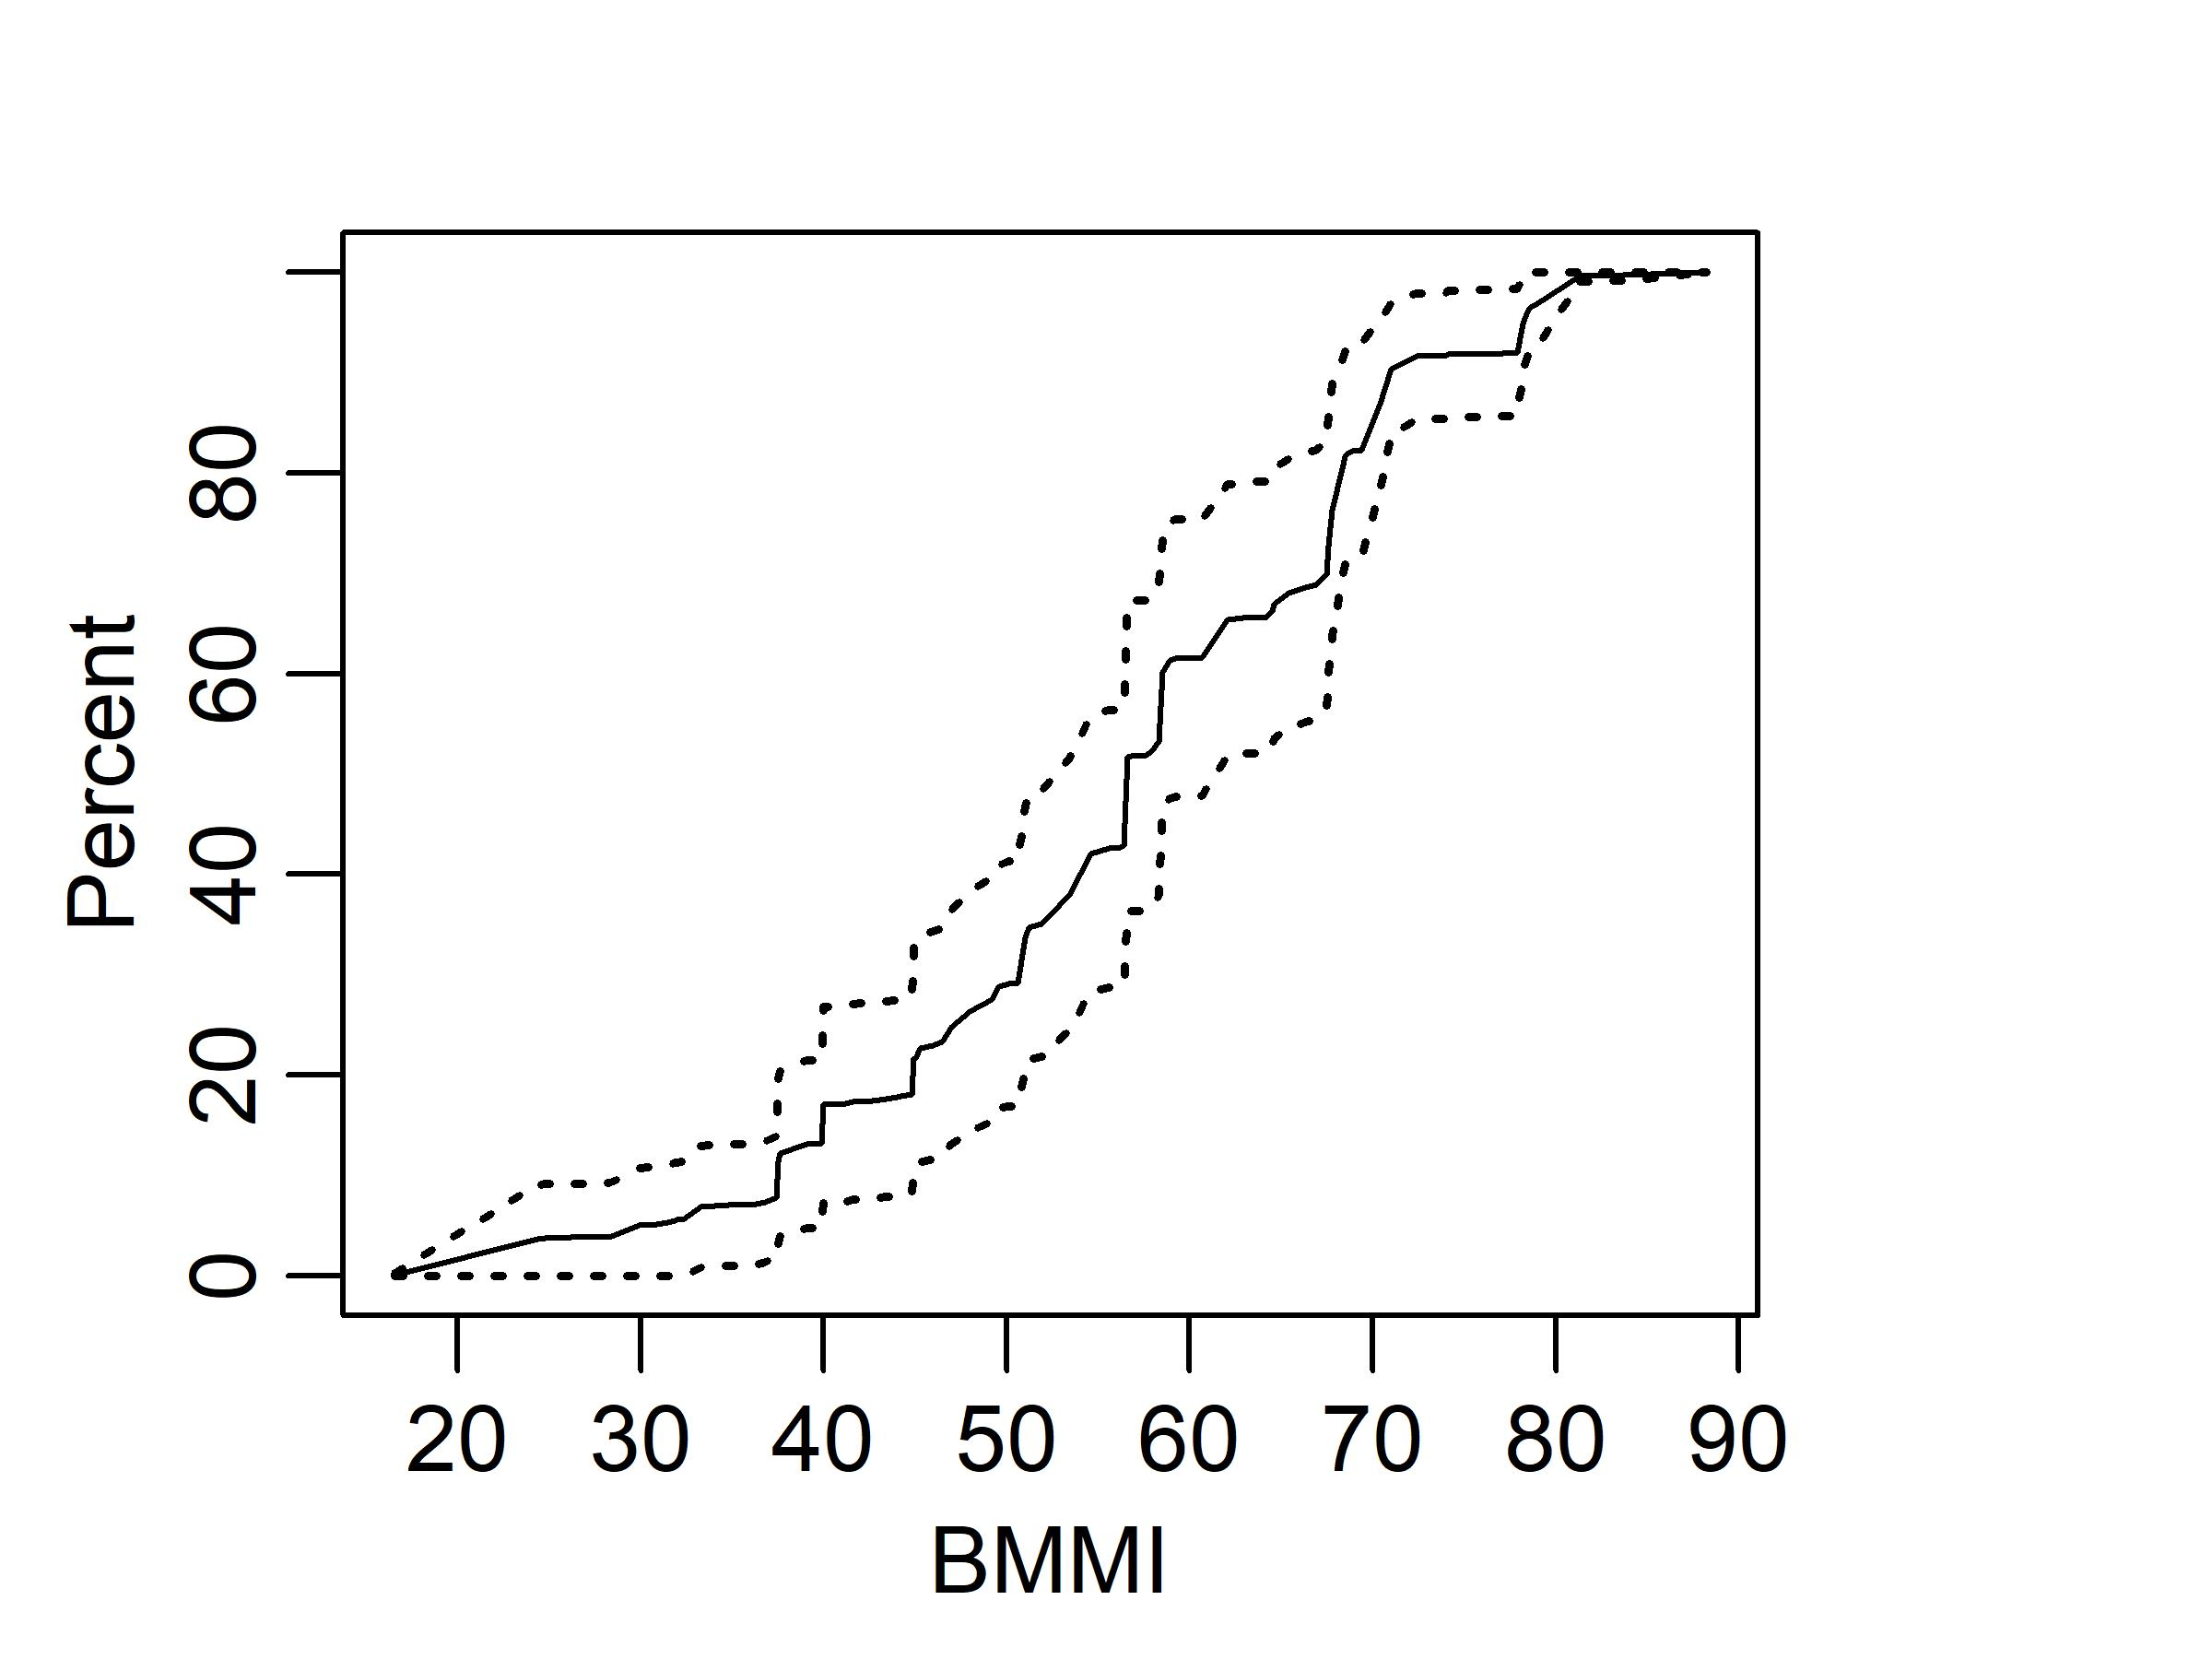
\includegraphics[width = 0.49\linewidth]{images/bmmi_cdf.jpeg}
\caption{BMMI cumulative distribution function (CDF) estimates (solid line) and 95\% confidence intervals (dashed lines).}
\label{fig:bmmi_cdf}
\end{figure}

The percentile output is contained in \texttt{bmmi\$Pct}. By default, a
few specific percentiles are estimated, though this can be changed via
the \code{pctval} argument.

To analyze \code{BMMI} separately for each state, run

\begin{CodeChunk}
\begin{CodeInput}
R> bmmi_state <- cont_analysis(
+   NLA_PNW, 
+   vars = "BMMI",
+   subpops = "STATE",
+   weight = "WEIGHT"
+ )
\end{CodeInput}
\end{CodeChunk}

To view the sample sizes, estimates, and 95\% confidence intervals for
the mean in each state, run

\begin{CodeChunk}
\begin{CodeInput}
R> subset(
+   bmmi_state$Mean,
+   select = c(Subpopulation, Indicator, nResp, Estimate, LCB95Pct, UCB95Pct)
+ )
\end{CodeInput}
\begin{CodeOutput}
  Subpopulation Indicator nResp Estimate LCB95Pct UCB95Pct
1    California      BMMI    19 50.48964 42.55357 58.42572
2        Oregon      BMMI    47 61.29675 56.23802 66.35548
3    Washington      BMMI    30 54.23036 48.06838 60.39234
\end{CodeOutput}
\end{CodeChunk}

To incorporate stratification (by urban category), run

\begin{CodeChunk}
\begin{CodeInput}
R> bmmi_strat <-  cont_analysis(
+   NLA_PNW,
+   vars = "BMMI",
+   stratumID = "URBAN",
+   weight = "WEIGHT"
+ )
\end{CodeInput}
\end{CodeChunk}

To incorporate subpopulations (by state) and stratification (by urban
category), run

\begin{CodeChunk}
\begin{CodeInput}
R> bmmi_strat_state <-  cont_analysis(
+   NLA_PNW,
+   vars = "BMMI",
+   subpops = "STATE",
+   stratumID = "URBAN",
+   weight = "WEIGHT",
+ )
\end{CodeInput}
\end{CodeChunk}

\hypertarget{additional-analysis-approaches}{%
\subsection{Additional analysis
approaches}\label{additional-analysis-approaches}}

Several other analysis options are available in \pkg{spsurvey}: relative
risk analysis using \linebreak \code{relrisk_analysis()}; attributable
risk analysis using \code{attrisk_analysis()}; difference in risk
analysis using \code{diffrisk_analysis()}; change analysis using
\code{change_analysis()}; and trend analysis using
\code{trend_analysis()}. The arguments for these functions are nearly
identical to the arguments for \code{cat_analysis()} and
\code{cont_analysis()}, with a few occasional exceptions.

The relative risk of an event (with respect to a stressor) is the ratio
of two quantities. The numerator of the ratio is the probability the
event occurs given exposure to the stressor. The denominator of the
ratio is the probability the event occurs given no exposure to the
stressor. Mathematically, the relative risk is defined as
\begin{align}\label{eq:rr}
  \text{RR} = \frac{P(\text{Event} | \text{Stressor})}{P(\text{Event} | \text{No Stressor})},
\end{align} where \(P(\text{Event} | \text{Stressor})\) is the
probability the event occurs given exposure to the stressor and
\(P(\text{Event} | \text{No Stressor})\) is the probability the event
occurs given no exposure to the stressor. The attributable risk of an
event (with respect to a stressor) is one minus a ratio of two
quantities. The numerator of the ratio is the probability the event
occurs given no exposure to the stressor. The denominator of the ratio
is the overall probability the event occurs. Mathematically, the
attributable risk is defined as\\
\begin{align}\label{eq:ar}
  \text{AR} = 1 - \frac{P(\text{Event} | \text{No Stressor})}{P(\text{Event})} ,
\end{align} where \(P(\text{Event})\) is the overall probability the
event occurs.

Though relative risk and attributable risk are most often discussed in
the medical literature, \citet{sickle2008assessing} emphasize the
usefulness of relative and attributable risk in the context of aquatic
resources and stressors. The final risk metric available in
\pkg{spsurvey} is difference in risk (with respect to a stressor). The
difference in risk is the difference between the probability the event
occurs given exposure to the stressor and the probability the event
occurs given no exposure to the stressor. Mathematically, the difference
in risk is defined as \begin{align}{\label{eq:rd}}
 \text{RD} = P(\text{Event} | \text{Stressor}) - P(\text{Event} | \text{No Stressor}) .
\end{align} Because it is not a relative metric, the difference in risk
complements the relative and attributable risks. The three risk metrics
quantify several different aspects of risk and together to help provide
a complete characterization of a resource's risk (with respect to a
stressor).

The risk analysis functions in \pkg{spsurvey} require four new
arguments: \code{vars_response}, which indicates the response variables;
\code{vars_stressor}, which indicates the stressor variables; \linebreak
\code{response_levels}, which indicates the two levels of the response
variables (event and no event); and \code{stressor_levels}, which
indicates the two levels of the stressor variables (stressor present and
stressor not present). If the \code{vars_response} and
\code{vars_stressor} arguments are vectors, all combinations of
\code{vars_response} and \code{vars_stressor} are analyzed.
Subpopulations and stratification are accommodated via the
\code{subpops} and \code{stratumID} arguments, respectively.

Change and trend estimation are most commonly used to study the behavior
of a resource through time. Change estimation focuses on comparing the
resource at two time points. Parameters are estimated at each time point
and the difference between the estimates is of interest. The variance of
this difference incorporates the variability at each time point and the
correlation between sites that are sampled at both time points. In trend
estimation, parameters are estimated at each time point and a regression
model fits a linear trend in the estimates through time. There are three
available regression models: a simple linear regression model, a
weighted linear regression model, and the mixed effects linear
regression model from \citet{piepho2002simple}.

The change and trend analysis functions in \pkg{spsurvey} require three
new arguments: \code{vars_cat}, which indicates the categorical
variables to estimate; \code{vars_cont}, which indicates the continuous
variables to estimate; and a \code{surveyID} variable that distinguishes
between the time points. The \code{trend_analysis()} function also
requires the \code{model_cat} and \code{model_cont} arguments, which
indicate the trend models for the categorical and continuous variables,
respectively. As with the risk analysis functions, subpopulations and
stratification are accommodated via the \code{subpops} and
\code{stratumID} arguments, respectively.

\hypertarget{sec:application}{%
\section{Application}\label{sec:application}}

In this section, we use \pkg{spsurvey} to compare two sampling and
analysis approaches: spatial and non-spatial. The spatial approach uses
the GRTS algorithm for sampling and the local neighborhood variance
estimator (Equation\(~\)\ref{eq:var_lnb}) for analysis. The non-spatial
approach uses simple random sampling (SRS) and its variance estimator
(Equation\(~\)\ref{eq:var_irs}) for analysis. The data studied are from
the United States Environmental Protection Agency's 2012 National Lakes
Assessment, a survey designed to monitor the status of lakes in the
conterminous United States in 2012 \citep{usepa2012NLA}.

We considered two variables in the NLA12 data: Atrazine presence (AP), a
binary metric indicating whether Atrazine is present; and a continuous
benthic macroinvertebrate multi-metric index (BMMI). Data were recorded
at 1028 lakes for AP and 914 lakes for BMMI. By running

\begin{CodeChunk}
\begin{CodeInput}
R> NLA12 <- sp_frame(NLA12)
R> summary(NLA12, formula = ~ AP + BMMI)
\end{CodeInput}
\begin{CodeOutput}
   total         AP           BMMI      
 total:1030   N   :694   Min.   : 0.00  
              Y   :334   1st Qu.:33.00  
              NA's:  2   Median :43.90  
                         Mean   :43.22  
                         3rd Qu.:54.60  
                         Max.   :86.10  
                         NA's   :116    
\end{CodeOutput}
\end{CodeChunk}

we see that the true proportion of lakes containing Atrazine is 0.3249,
and the true mean BMMI of lakes is 43.22. By running

\begin{CodeChunk}
\begin{CodeInput}
R> plot(NLA12, formula = ~ AP + BMMI)
\end{CodeInput}
\end{CodeChunk}

we see that Atrazine presence is concentrated in the Upper Midwest
(Figure\(~\)\ref{fig:atrazine}), while there is no clear spatial pattern
for \code{BMMI} (Figure\(~\)\ref{fig:bmmi}). The data for each resource
are treated as separate populations for the purposes of this section.

\begin{figure}
\centering
\begin{subfigure}{0.49\textwidth}
  \centering
  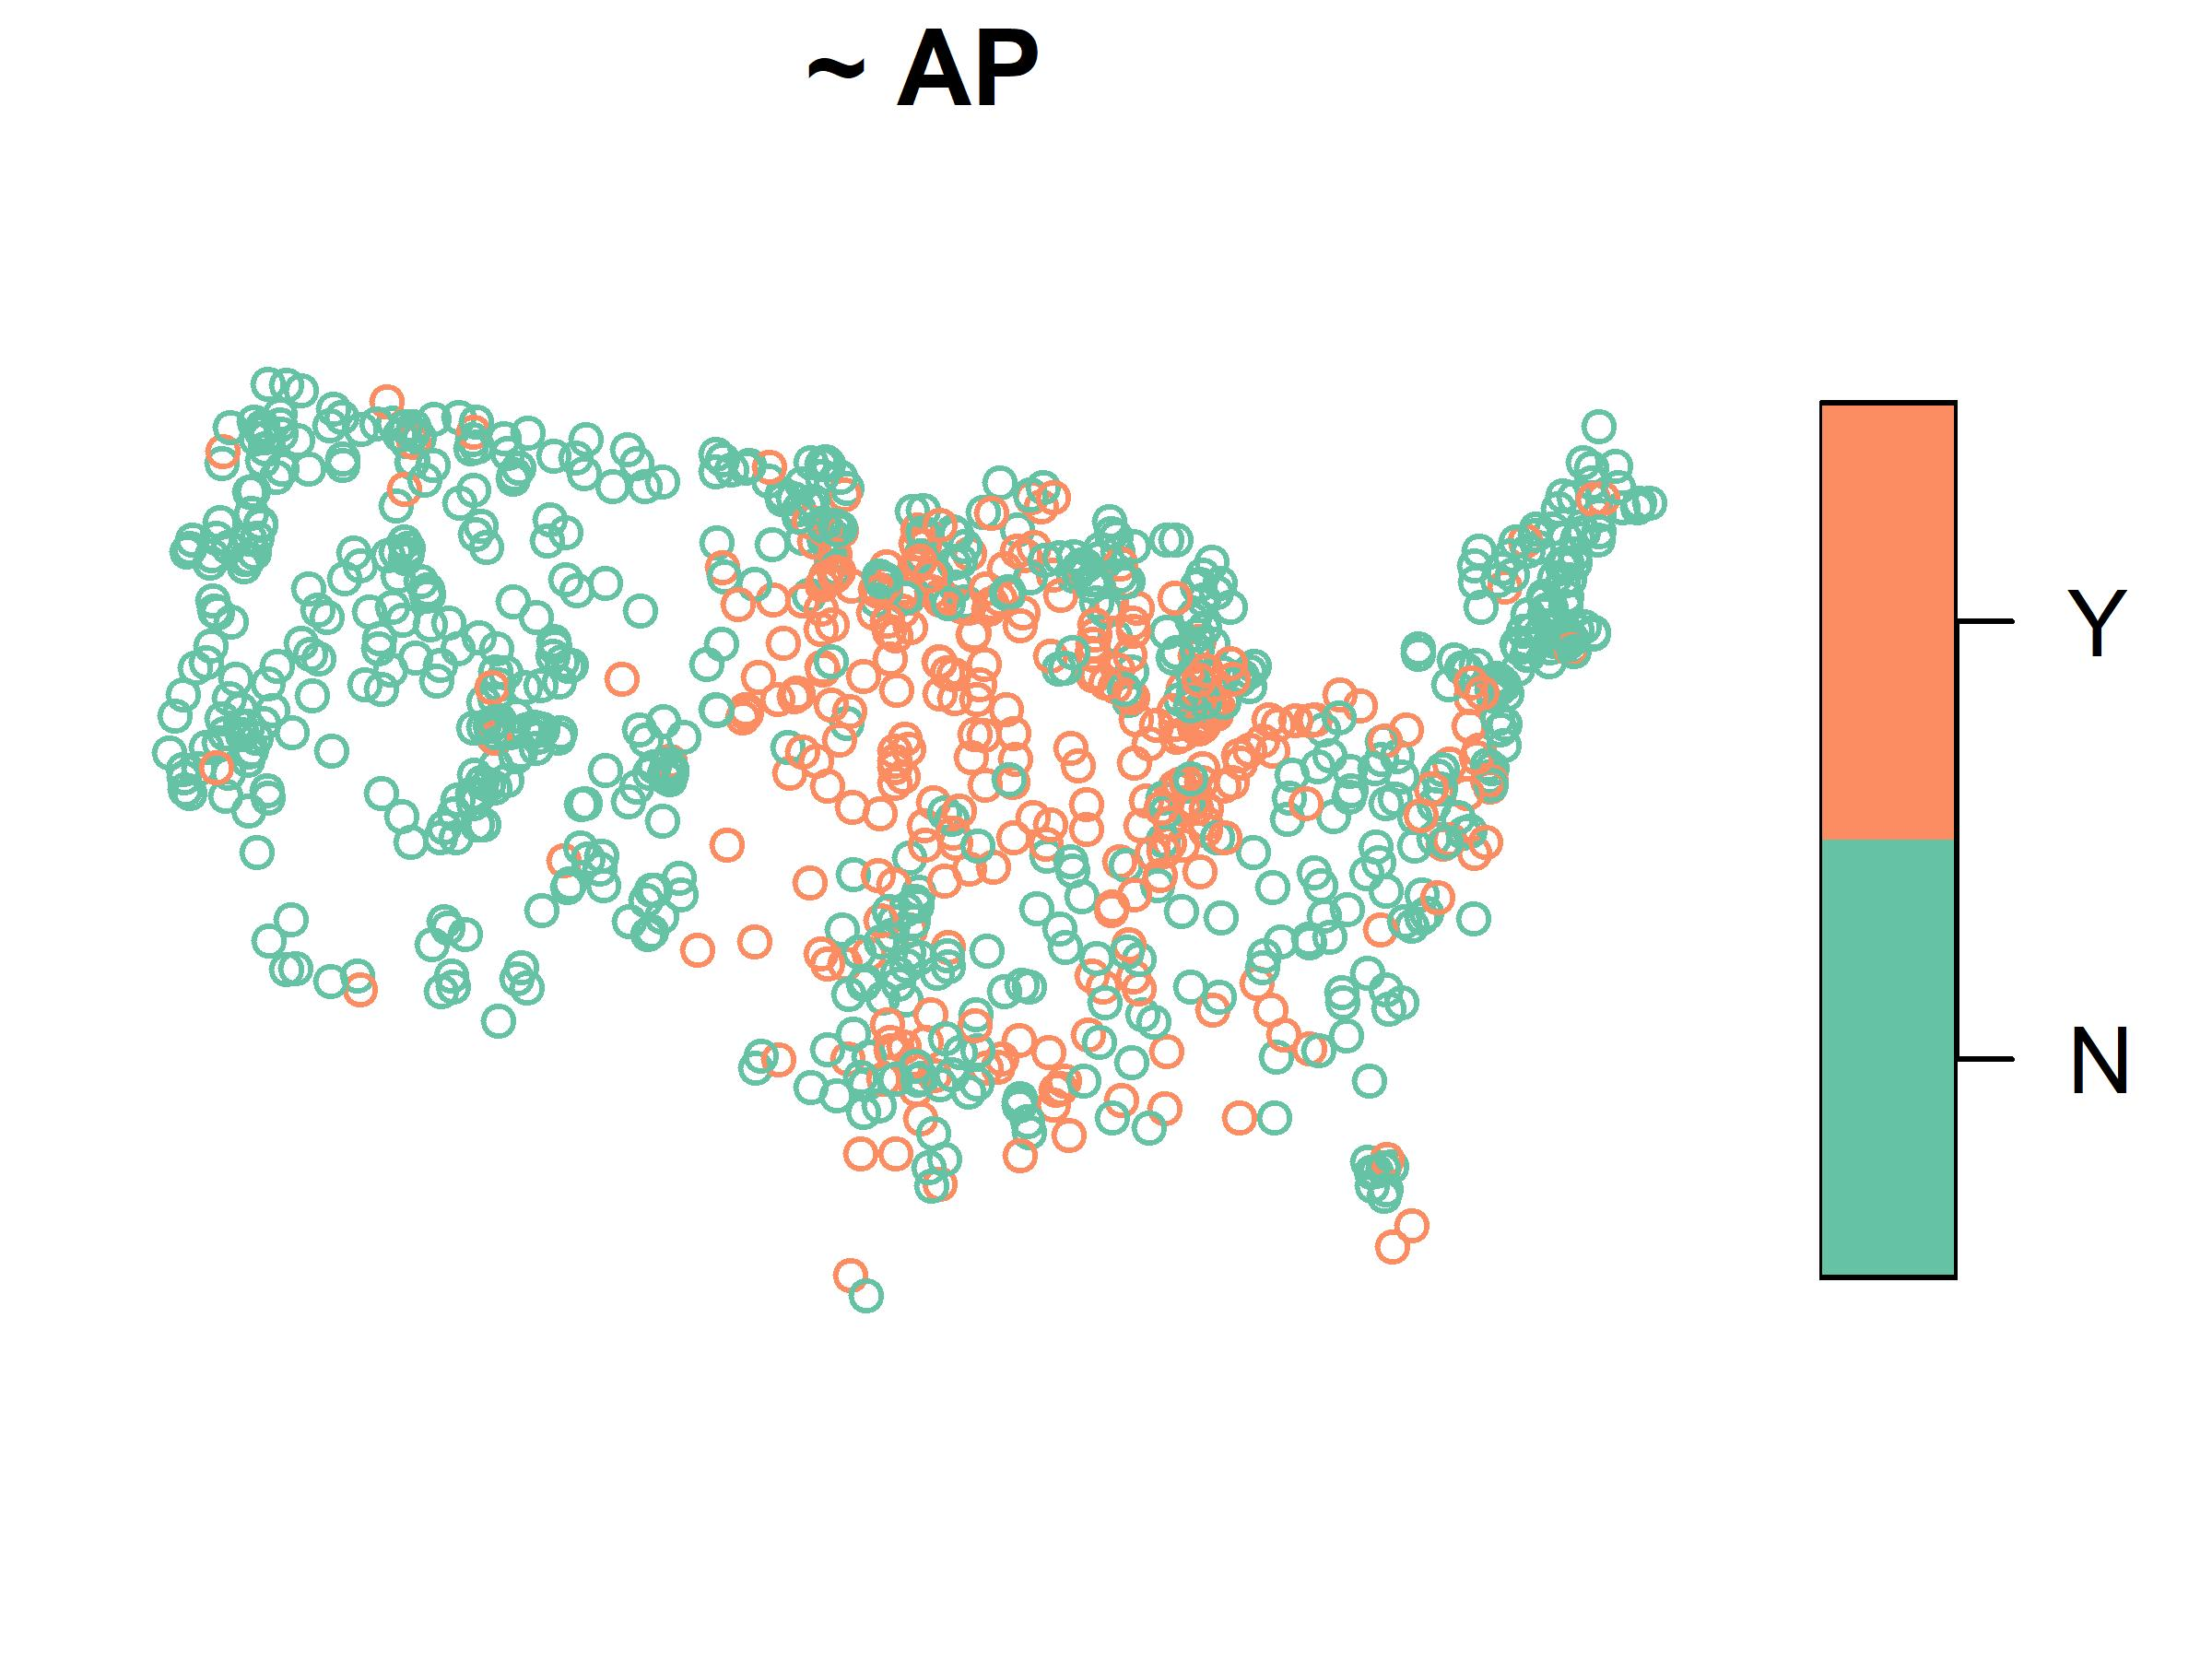
\includegraphics[width = 1\linewidth]{images/atrazine.jpeg}
  \caption{}
  \label{fig:atrazine}
\end{subfigure}
\begin{subfigure}{0.49\textwidth}
  \centering
  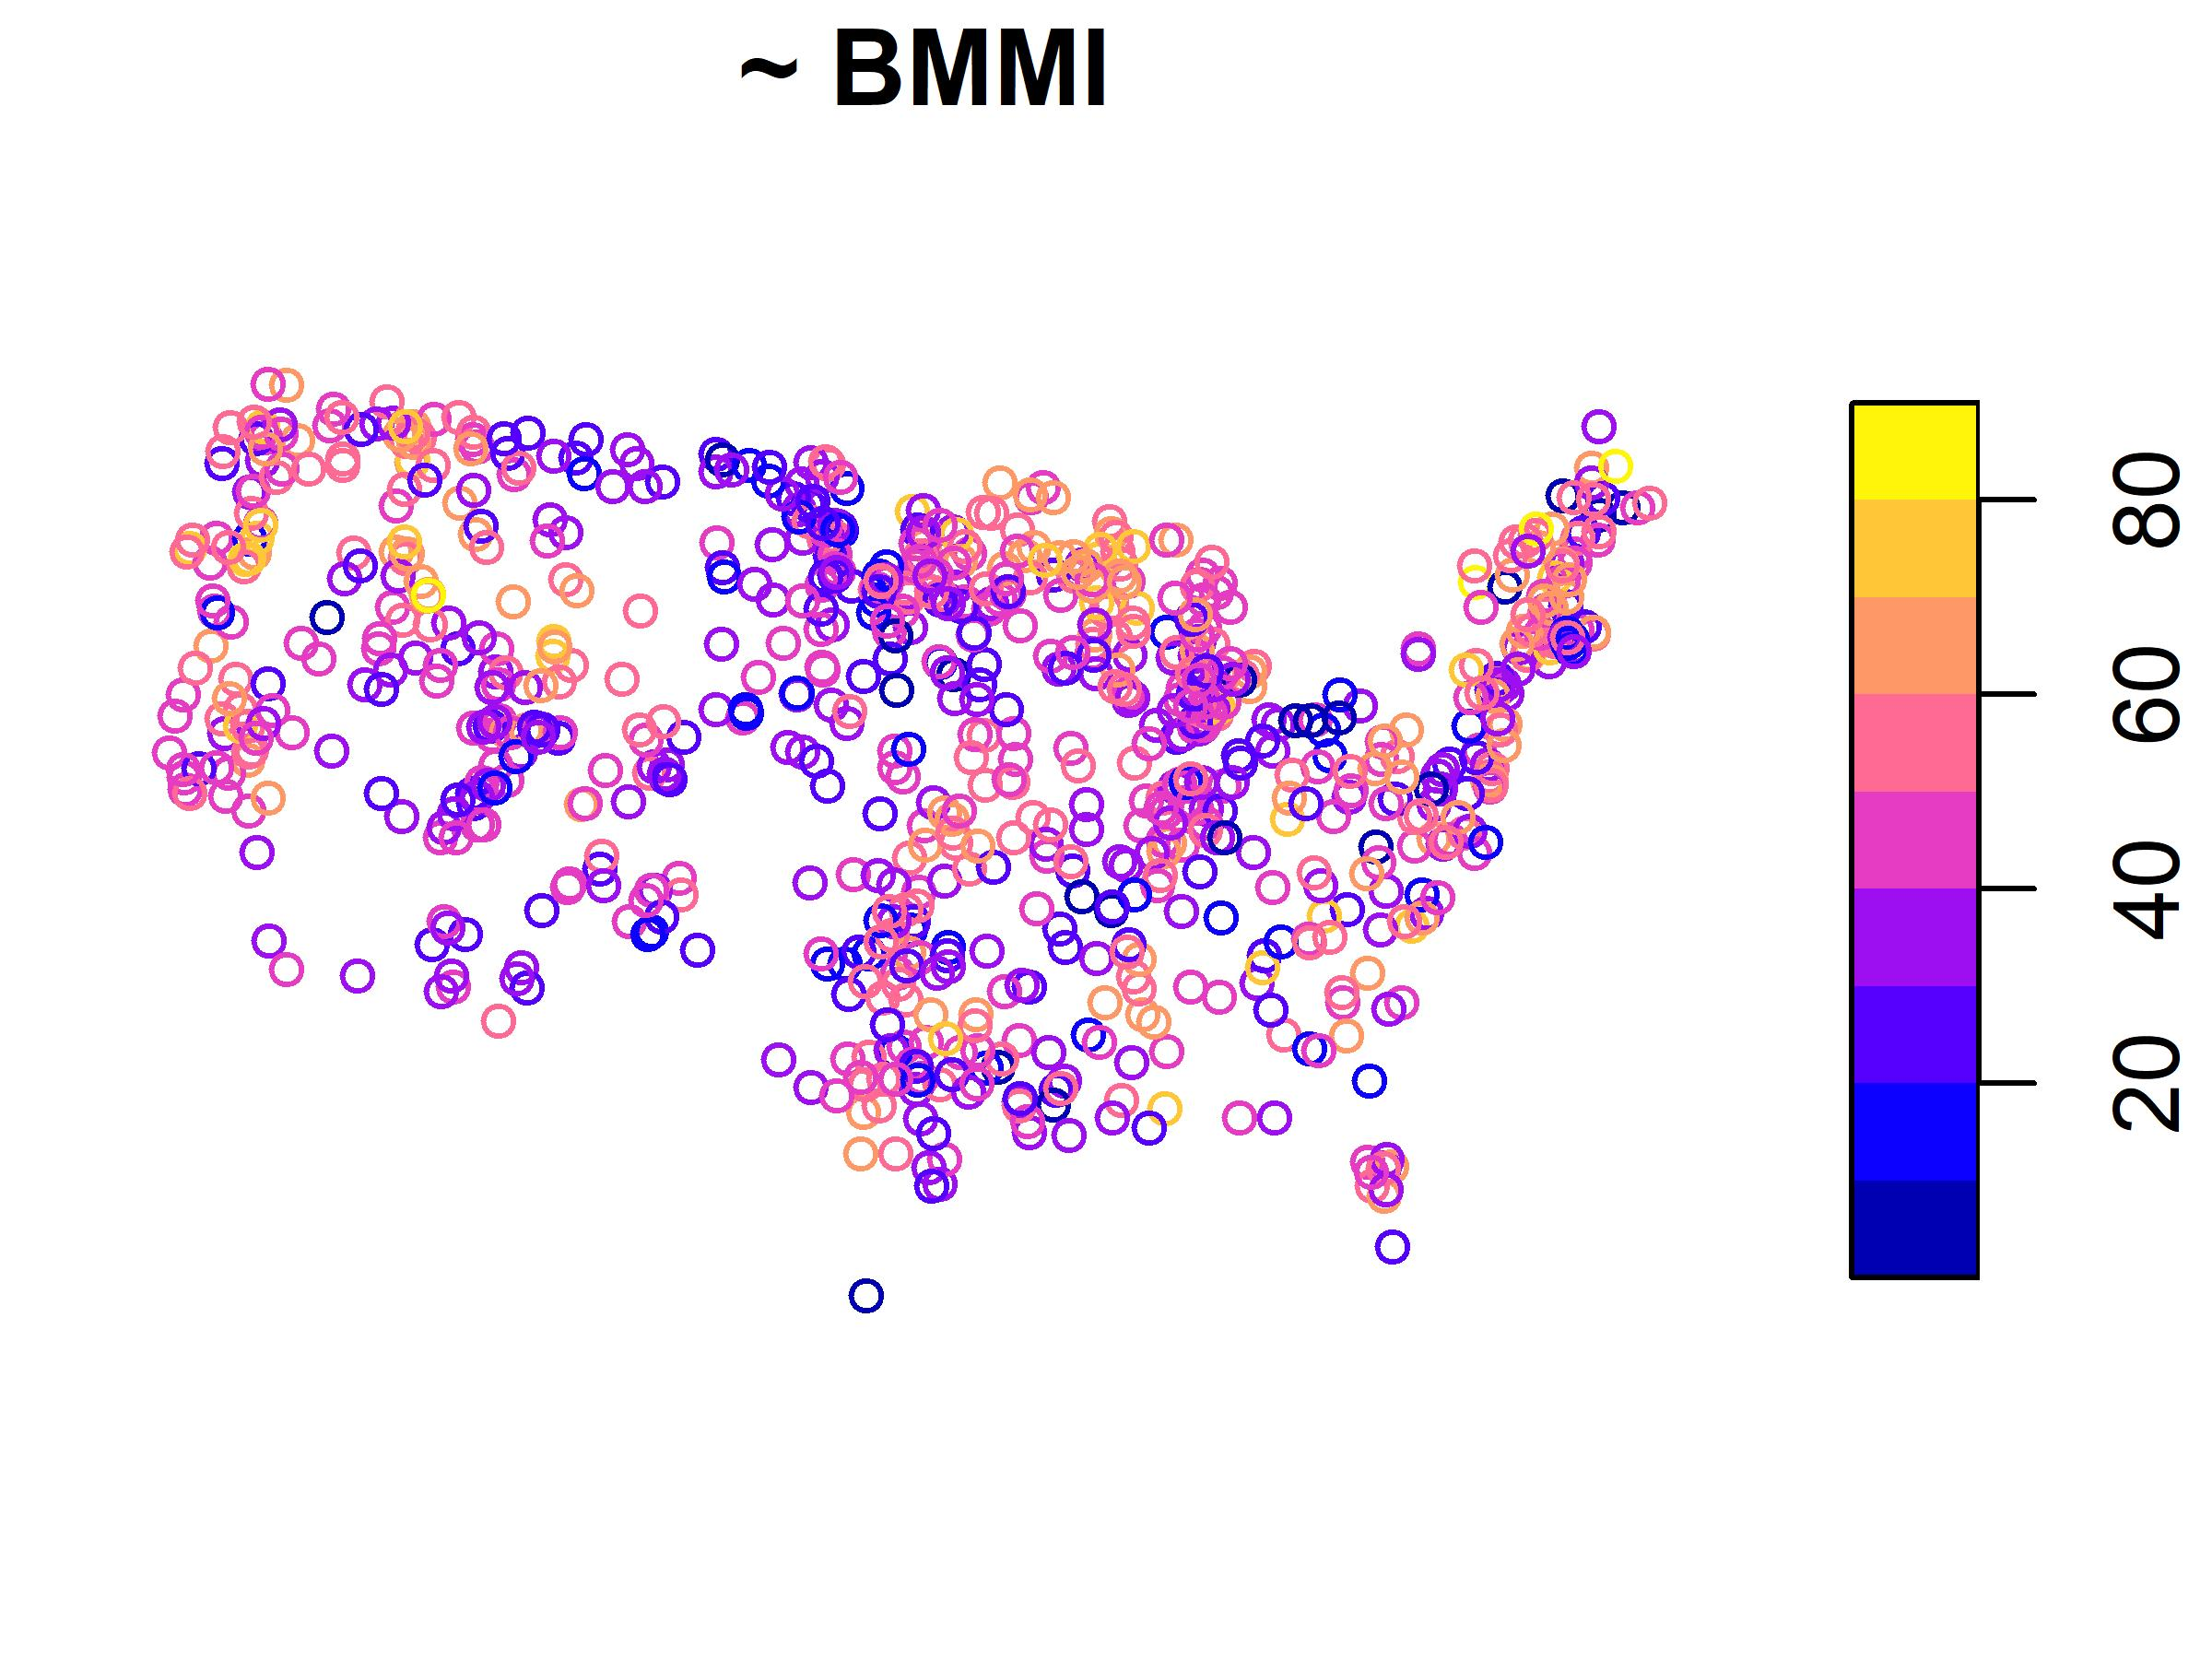
\includegraphics[width = 1\linewidth]{images/bmmi.jpeg}
  \caption{}
  \label{fig:bmmi}
\end{subfigure} 
\caption{Spatial distributions of Atrazine presence (a) and a benthic macroinvertebrate multi-metric index (b) from the 2012 National Lakes Assessment.}
\label{fig:simvars}
\end{figure}

A simulation study was used to compare the spatial and non-spatial
approaches. First unstratified, equal probability samples of size 250
were selected from the Atrazine presence population
(Figure\(~\)\ref{fig:atrazine}) using the GRTS and SRS algorithms. Then
several quantities were computed: the sample's spatial balance measured
using Pielou's evenness index; an estimate, denoted by \(\hat{p}\), of
the true proportion of Atrazine presence, denoted by \(p\); an estimate
of the standard error of \(\hat{p}\); and an indicator variable
measuring whether a 95\% confidence interval for \(p\) contains 0.3249.
This process was repeated 2000 times, and then the following summary
metrics were computed: mean spatial balance; mean bias, measured as the
average deviation of \(\hat{p}\) from \(p\); root-mean-squared error,
measured as the square root of the average squared deviation of
\(\hat{p}\) from \(p\); the 95\% confidence interval coverage rate; and
mean margin of error, measured as the average half-width of the 95\%
confidence interval for \(p\). The same process was used to study BMMI.
The \pkg{spsurvey} functions \code{grts()}, \code{irs()},
\code{sp_balance()}, \code{cat_anlaysis()}, and \code{cont_analysis()}
were used during these simulations.

The Atrazine presence summary metrics are presented in
Table\(~\)\ref{tab:atrazine_tab}. The mean spatial balance for the GRTS
samples is lower than for the SRS samples. The Atrazine presence
estimates from the GRTS and SRS samples both appear to be unbiased (mean
bias near zero), but the root-mean-squared error of the SRS estimates is
roughly 25\% higher than root-mean-squared error of the GRTS estimates.
The spatial approach and the non-spatial approach both have confidence
interval coverage near 95\%. The mean margin of error for the
non-spatial approach, however, is roughly 24\% higher than for the
spatial approach. Boxplots representing each simulation trial's spatial
balance and margin of error are displayed for both approaches in
Figure\(~\)\ref{fig:cat}.

\begin{table}[t!]
\centering
\begin{tabular}{lrrrrr}
  \hline
Algorithm & SPB & Bias & RMSE & Coverage & MOE \\ 
  \hline
GRTS & 0.0214 & -0.0003 & 0.0206 & 0.9525 & 0.0406 \\ 
  SRS & 0.0339 & -0.0008 & 0.0258 & 0.9455 & 0.0505 \\ 
   \hline
\end{tabular}
\caption{Sampling algorithm (Algorithm), mean spatial balance (SPB), mean bias (Bias), root-mean-squared error (RMSE), 95\% confidence interval coverage (Coverage), and mean margin of error (MOE) for 2000 simulation trials comparing the spatial and non-spatial approaches for studying Atrazine presence.} 
\label{tab:atrazine_tab}
\end{table}

\begin{figure}
\centering
\begin{subfigure}{0.45\textwidth}
  \centering
  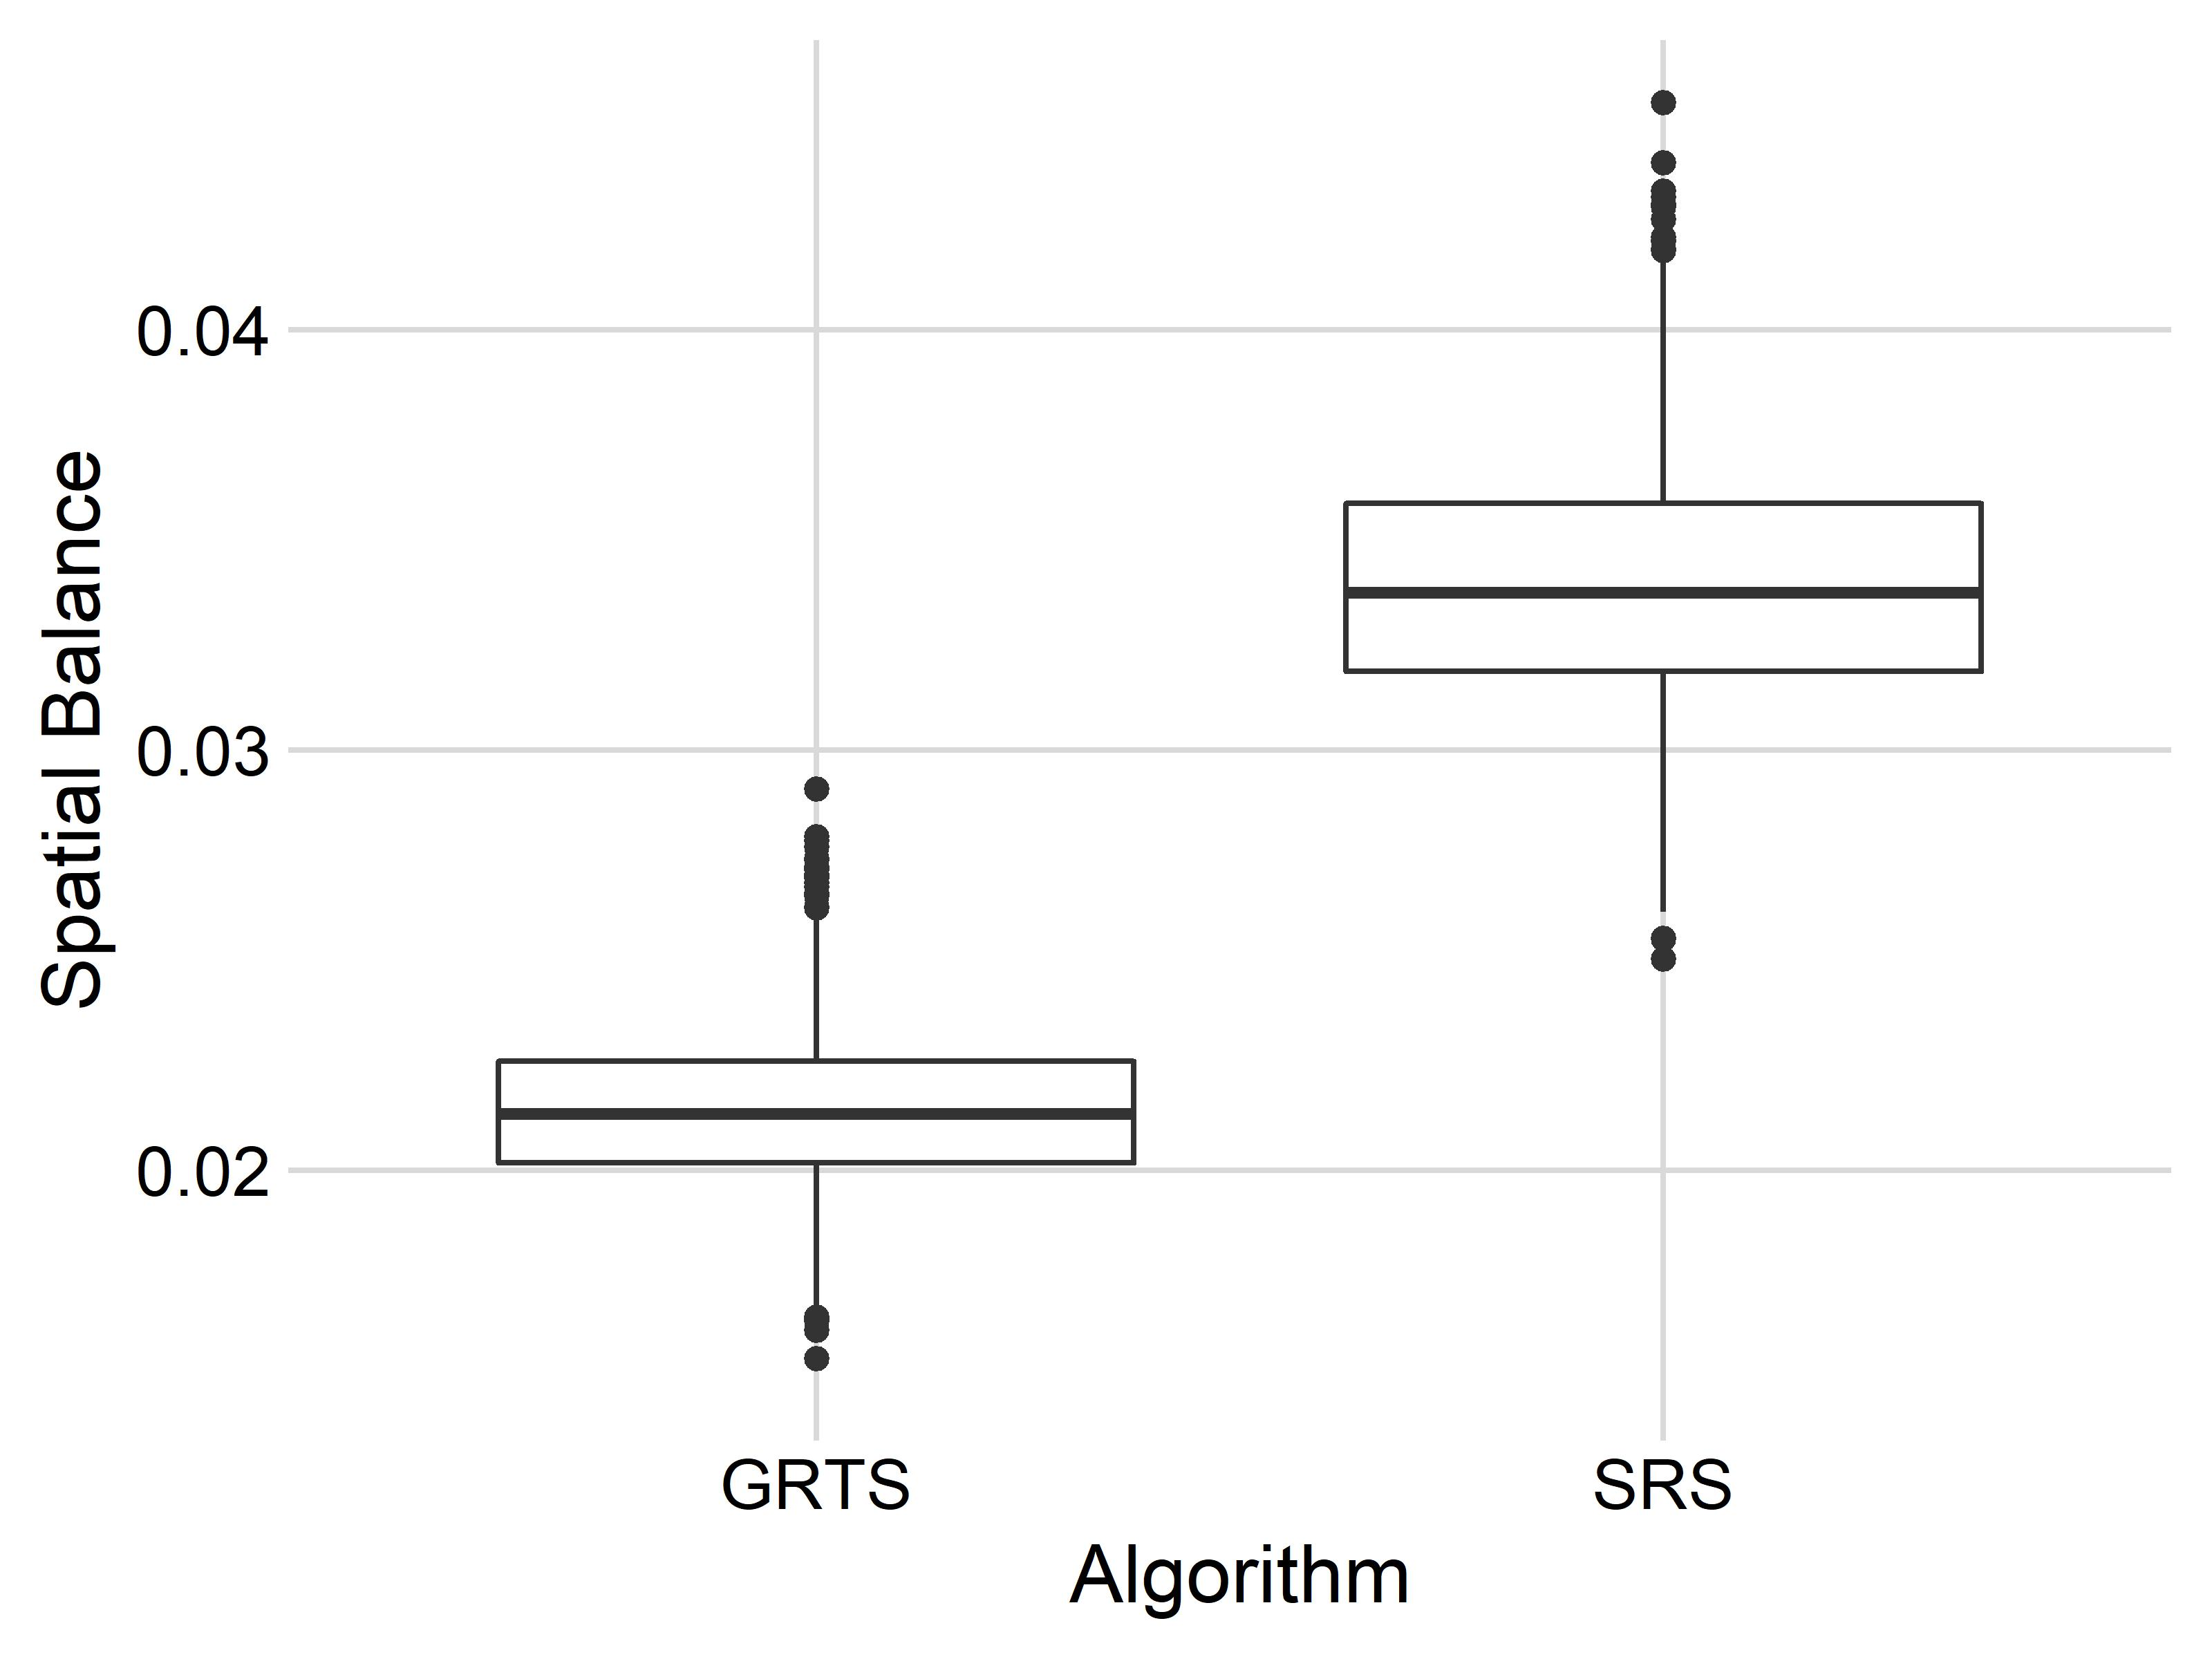
\includegraphics[width = 1\linewidth]{images/cat_spb.jpeg}
  \caption{}
  \label{fig:cat_moe}
\end{subfigure}
\begin{subfigure}{0.45\textwidth}
  \centering
  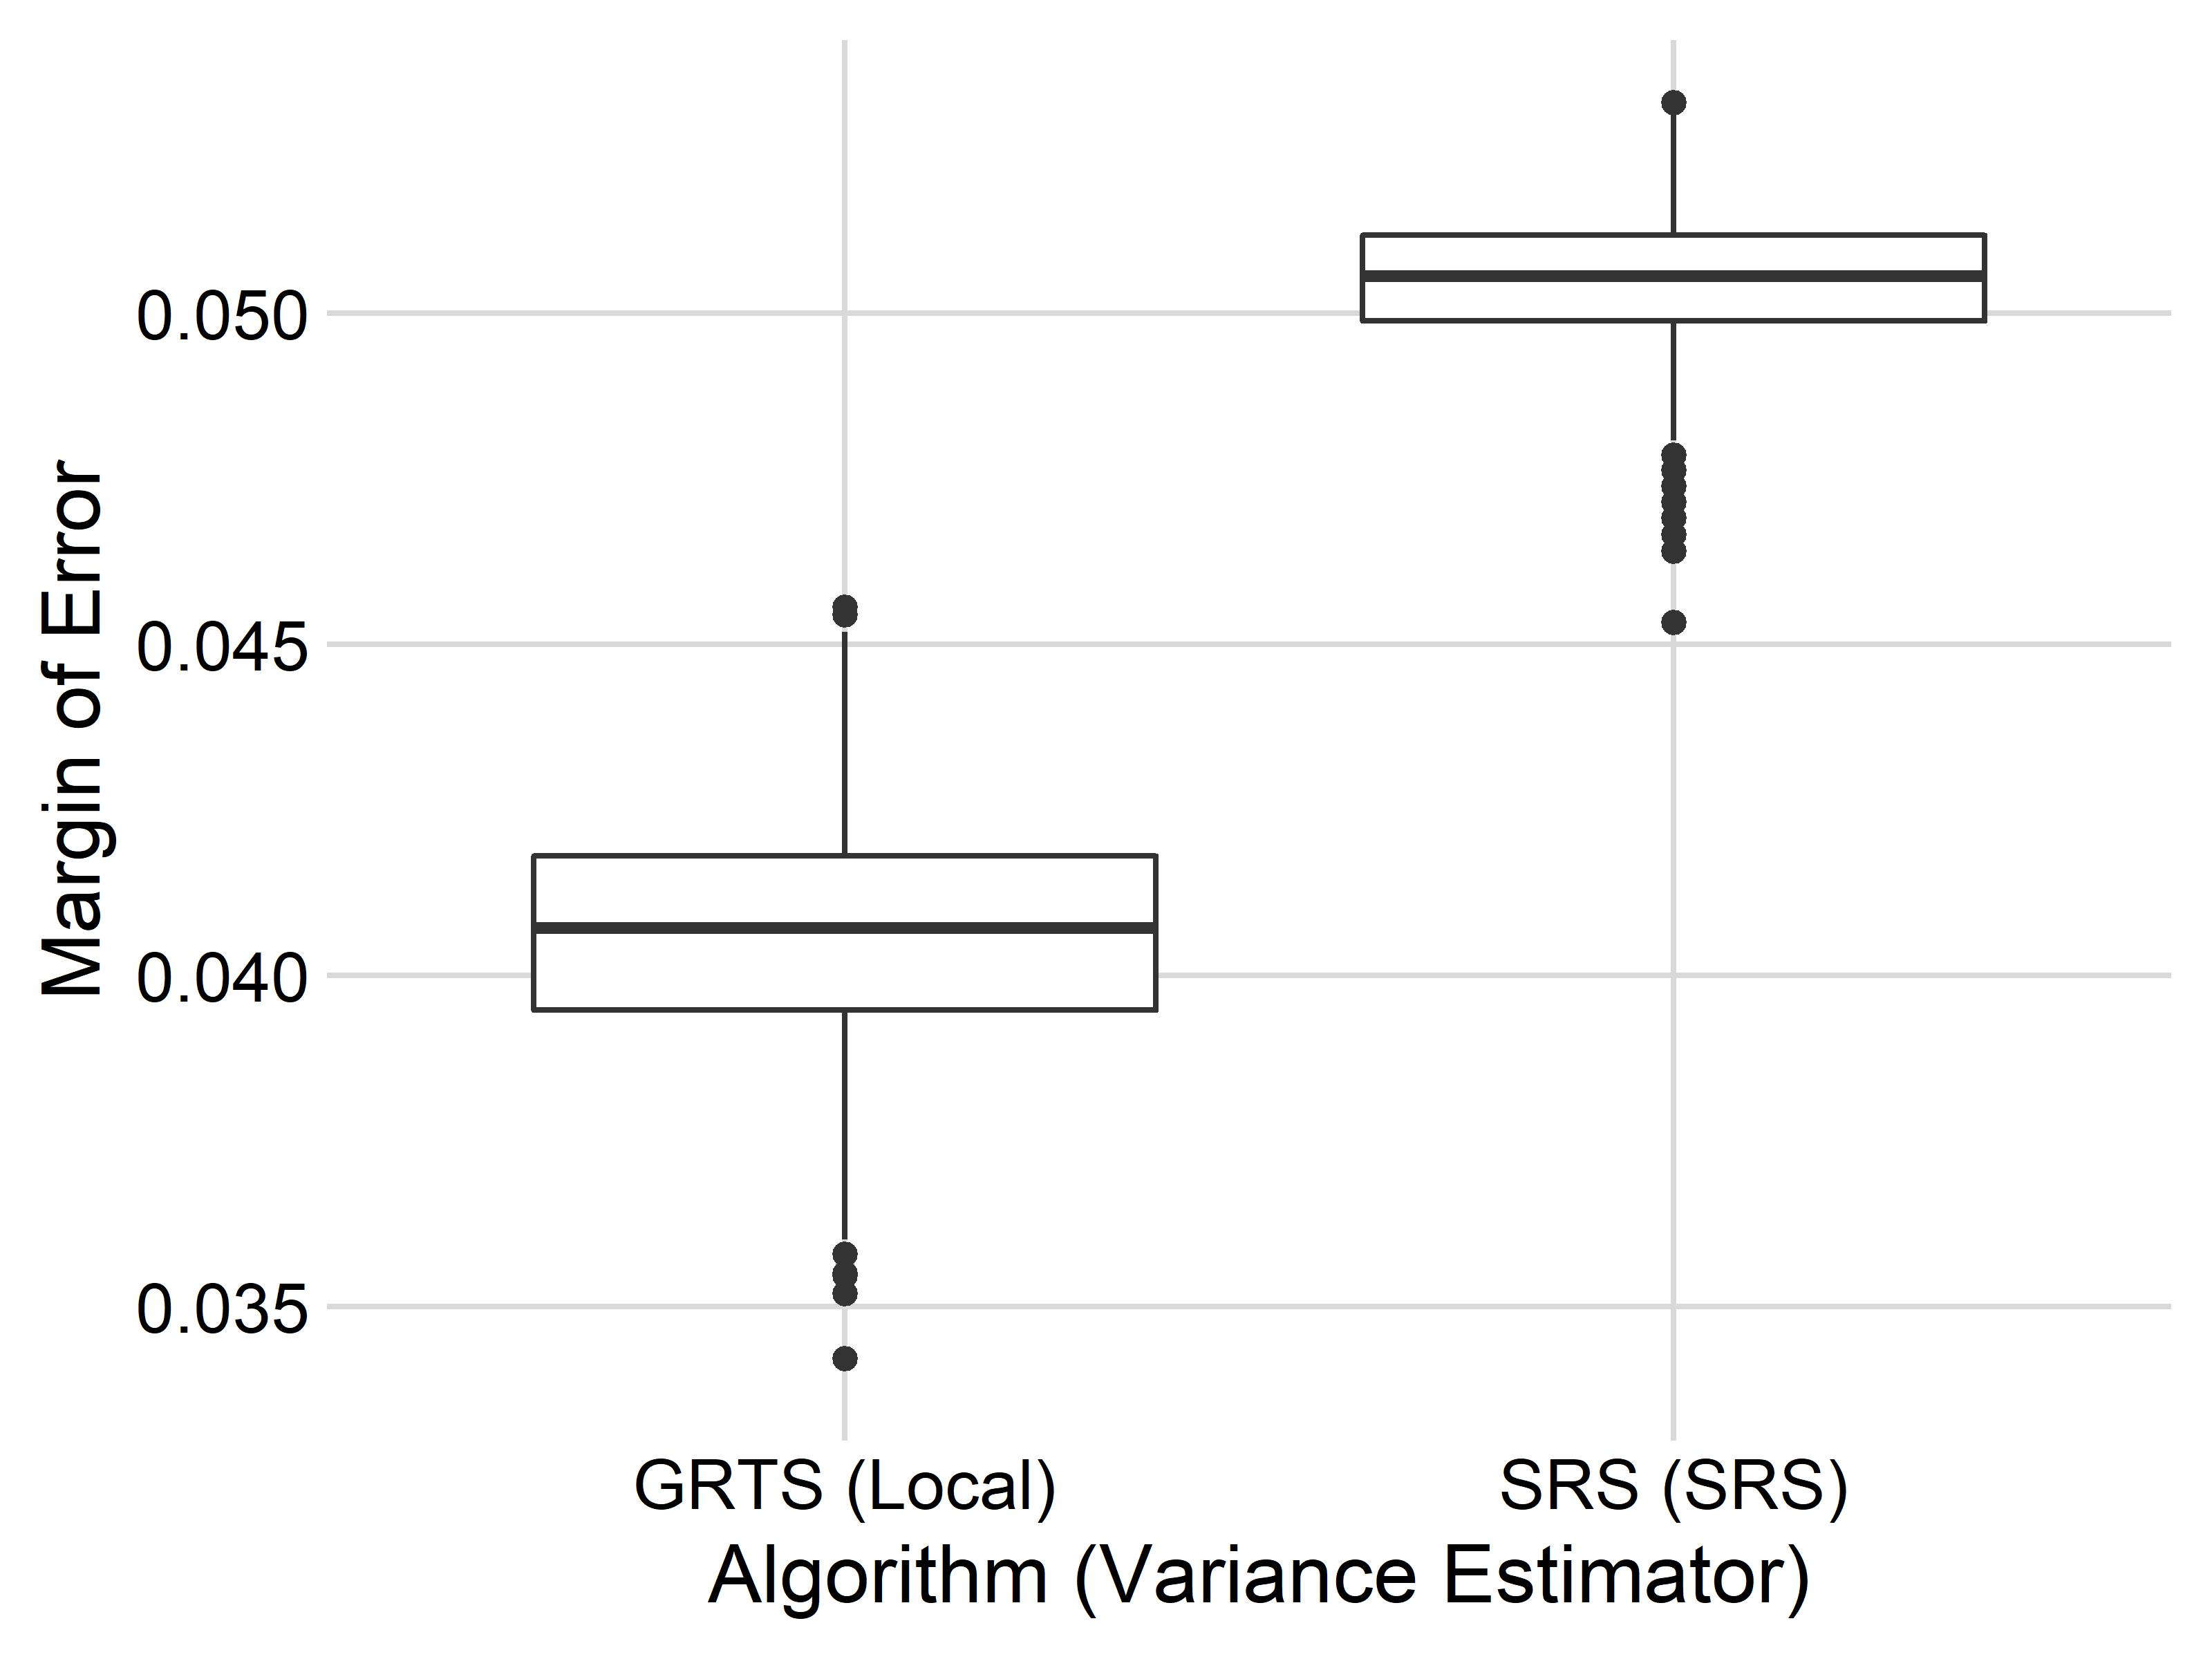
\includegraphics[width = 1\linewidth]{images/cat_moe.jpeg}
  \caption{}
  \label{fig:cat_spb}
\end{subfigure}
\caption{Boxplots of spatial balance (a) and margins of error (b) in the 2000 simulation trials comparing the spatial and non-spatial approaches for studying Atrazine presence.}
\label{fig:cat}
\end{figure}

The BMMI summary metrics are presented in Table\(~\)\ref{tab:bmmi_sim}.
These results are similar to the Atrazine presence results: GRTS samples
tend be more spatially balanced than SRS samples; the mean bias of
estimates from the GRTS and SRS samples is near zero; root-mean-squared
error from the SRS samples is roughly 10\% higher than root-mean-squared
error from the GRTS samples; confidence interval coverage is near 95\%
for both approaches; and the mean margin of error for the non-spatial
approach is roughly 9\% higher than the mean margin of error for the
spatial approach. Boxplots representing each simulation trial's spatial
balance and margin of error are displayed for both approaches in
Figure\(~\)\ref{fig:cont}.

\begin{table}[t!]
\centering
\begin{tabular}{lrrrrr}
  \hline
Algorithm & SPB & Bias & RMSE & Coverage & MOE \\ 
  \hline
GRTS & 0.0213 & 0.0063 & 0.7655 & 0.9520 & 1.5303 \\ 
  SRS & 0.0336 & 0.0134 & 0.8421 & 0.9440 & 1.6668 \\ 
   \hline
\end{tabular}
\caption{Samplilng algorithm (Algorithm), mean spatial balance (SPB), mean bias (Bias), root-mean-squared error (RMSE), 95\% confidence interval coverage (Coverage), and mean margin of error (MOE) for 2000 simulation trials comparing the spatial and non-spatial approaches for studying BMMI.} 
\label{tab:bmmi_sim}
\end{table}

\begin{figure}
\centering
\begin{subfigure}{0.45\textwidth}
  \centering
  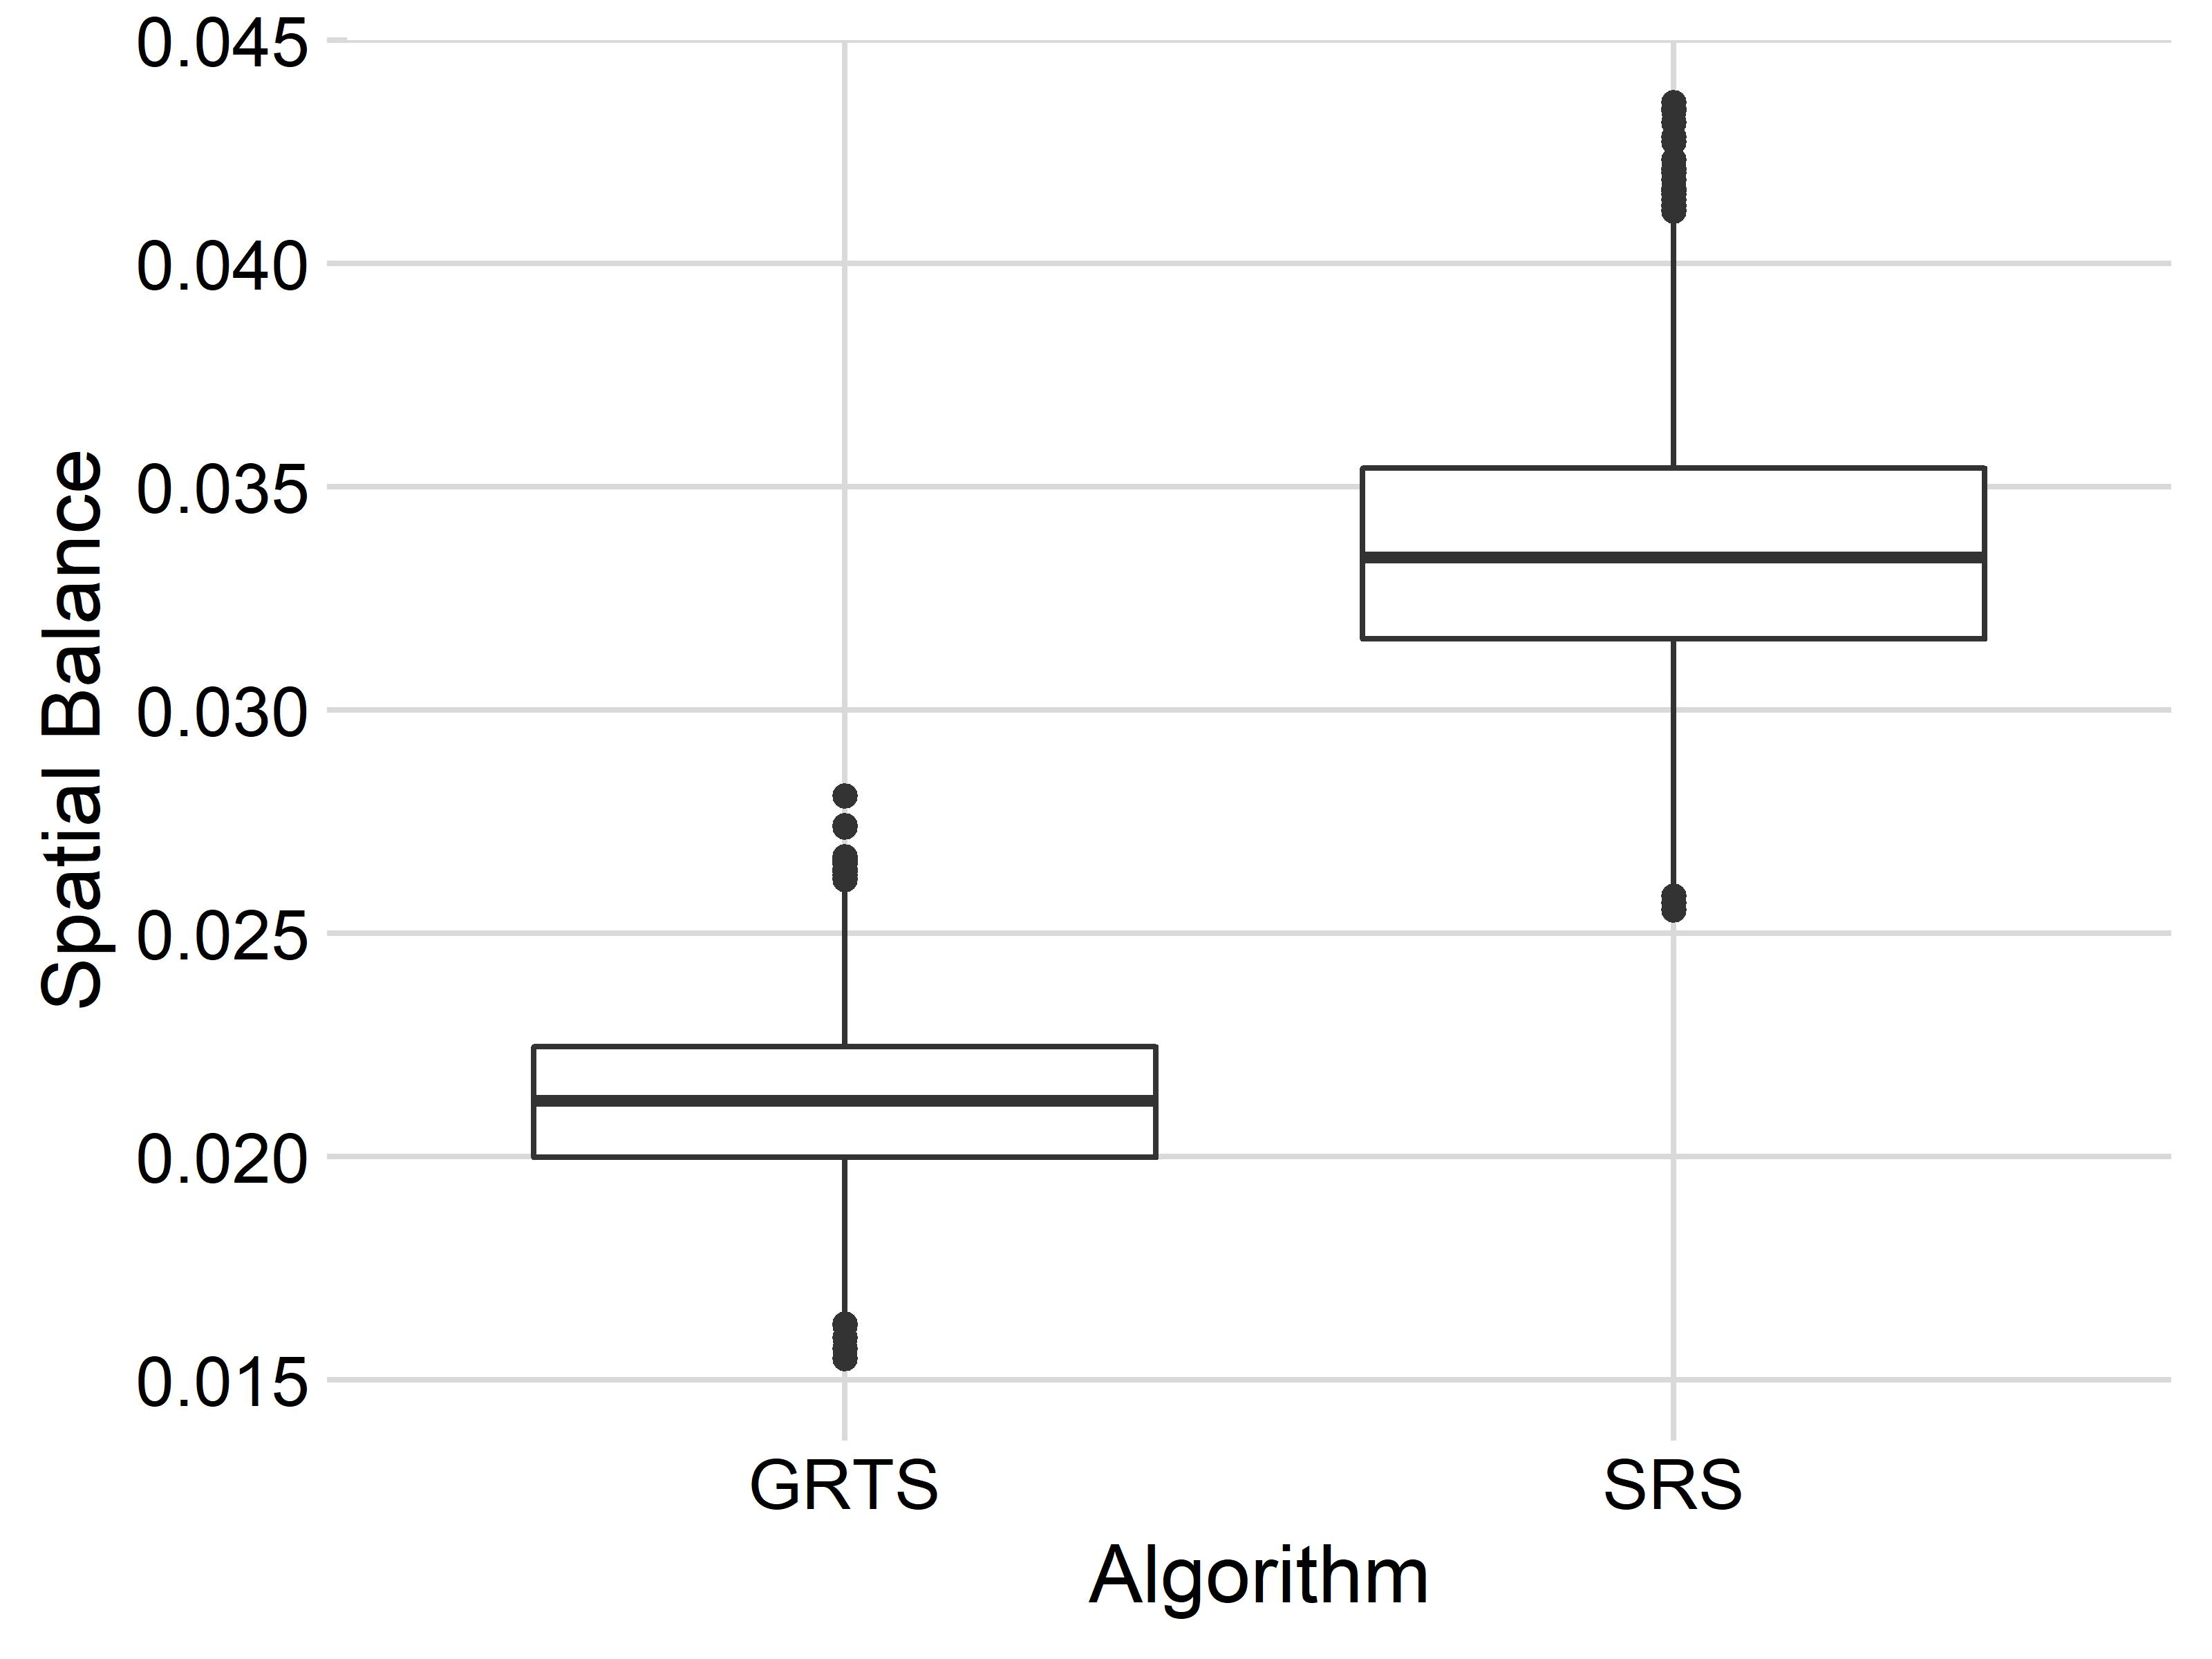
\includegraphics[width = 1\linewidth]{images/cont_spb.jpeg}
  \caption{}
  \label{fig:cont_moe}
\end{subfigure}
\begin{subfigure}{0.45\textwidth}
  \centering
  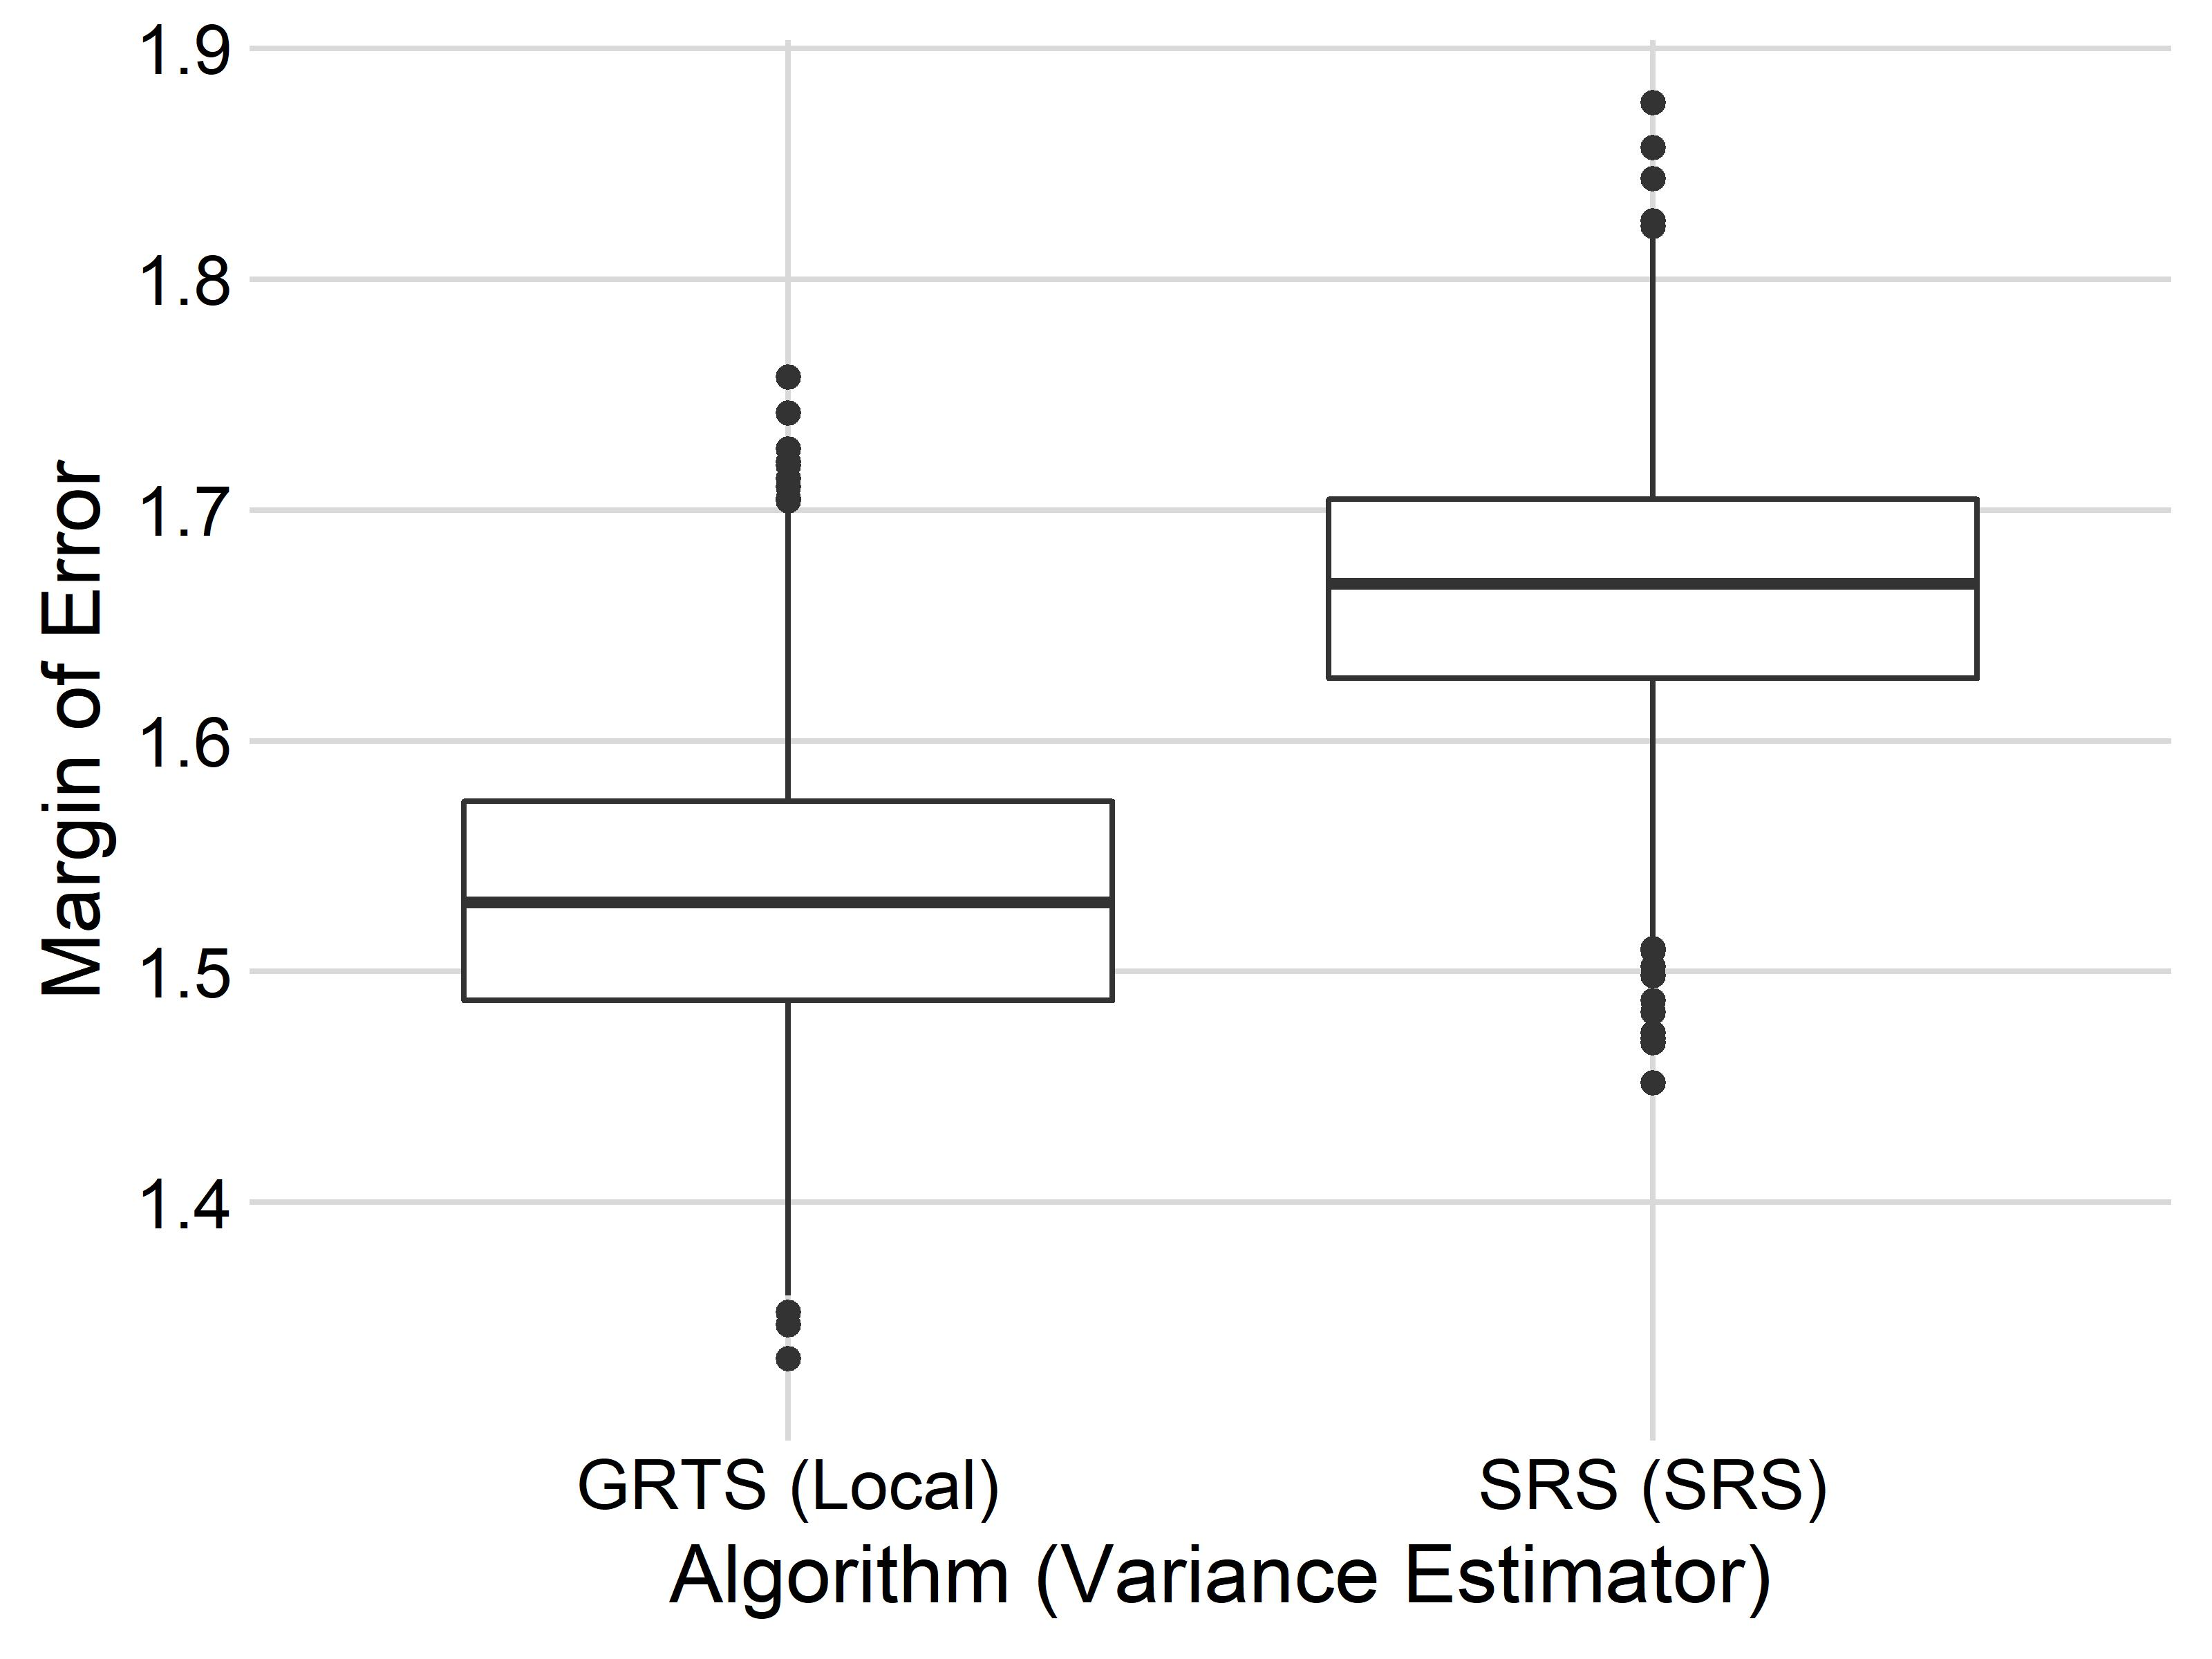
\includegraphics[width = 1\linewidth]{images/cont_moe.jpeg}
  \caption{}
  \label{fig:cont_spb}
\end{subfigure}
\caption{Boxplots of spatial balance (a) and margins of error (b) for 2000 simulation trials comparing the spatial and non-spatial approaches for studying BMMI.}
\label{fig:cont}
\end{figure}

The advantages of the spatial approach in this simulation study are
clear. The GRTS samples are more spatially balanced than the SRS
samples. The estimates from the GRTS samples are unbiased and have lower
root-mean-squared error than estimates from the SRS samples. The spatial
approach has smaller margins of error than the non-spatial approach
(while retaining proper coverage). This implies that confidence
intervals from the spatial approach are narrower (more precise) than
confidence intervals from the non-spatial approach.

For Atrazine presence, the non-spatial approach has a roughly 25\%
higher root-mean-squared error than the spatial approach. For BMMI, the
non-spatial approach have a roughly 10\% higher root-mean-squared error
than the spatial approach. The relative root-mean-squared error increase
is larger for Atrazine presence than BMMI. This is likely because
Atrazine presence has a stronger spatial pattern
(Figure\(~\)\ref{fig:atrazine}) than BMMI (Figure\(~\)\ref{fig:bmmi}),
suggesting that the stronger the spatial pattern, the greater the
advantage of the spatial approach compared to the non-spatial approach.

\hypertarget{sec:discussion}{%
\section{Discussion}\label{sec:discussion}}

\pkg{spsurvey} offers a suite of tools for design-based statistical
inference, with a focus on spatial data. The \code{summary()} and
\code{plot()} functions summarize and visualize data. The \code{grts()}
function selects spatially balanced samples from point, linear, and
areal resources and flexibly accommodates stratification, varying
inclusion probabilities, legacy (historical) sites, minimum distance
between sites, and two options for replacement sites (reverse
hierarchical ordering and nearest neighbor). The \code{sp_balance()}
function computes the spatial balance of a sample. The \code{sp_rbind()}
binds together the design sites into a single \pkg{sf} object.
\pkg{spsurvey}'s analysis functions are used for categorical variable
analysis (\code{cat_analysis()}), continuous variable analysis
(\code{cont_analysis()}), relative risk analysis
(\code{relrisk_analysis}), attributable risk analysis
(\code{attrisk_analysis()}), difference in risk analysis
(\code{diffrisk_analysis}), change analysis (\code{change_analysis}),
and trend analysis (\code{trend_analysis}). Aside from these core
functions, \pkg{spsurvey} has several other specialized functions to
perform cluster sampling and analysis, cumulative distribution function
(CDF) hypothesis testing, panel designs, power analysis, design weight
adjustments, and more.

We plan to continually update \pkg{spsurvey} so that it is reflective of
new research. Because \pkg{spsurvey} depends on \pkg{sf} for sampling
and \pkg{survey} \citep{lumley2020survey} for analysis, \pkg{spsurvey}
may also change alongside these packages. \pkg{spsurvey} is an
open-source project, and we want it to be as helpful and user-friendly
as possible. To help us accomplish these goals, we encourage users to
give us feedback regarding desired features, bug fixes, and other
suggestions for \pkg{spsurvey}.

\hypertarget{data-and-code-availability}{%
\section*{Data and code availability}\label{data-and-code-availability}}
\addcontentsline{toc}{section}{Data and code availability}

All writing, code, and data associated with this manuscript are
available for viewing and download in a supplementary \proglang{R}
package located at the GitHub repository:

\url{https://github.com/michaeldumelle/DumelleEtAl2021spsurvey}

Instructions for use are included in the repository's \code{README}.
This supplementary \proglang{R} package contains a replication script
that can be used to reproduce all results presented in the manuscript.
Replicating the simulation study could take 10 - 60 minutes, but results
are provided as \code{.rda} files in the supplementary \proglang{R}
package.

\hypertarget{acknowledgements}{%
\section*{Acknowledgements}\label{acknowledgements}}
\addcontentsline{toc}{section}{Acknowledgements}

We thank the editors and anonymous reviewers for their hard work and
time spent providing us with thoughtful, valuable feedback which greatly
improved the manuscript.

The views expressed in this manuscript are those of the authors and do
not necessarily represent the views or policies of the U.S.
Environmental Protection Agency. Any mention of trade names, products,
or services does not imply an endorsement by the U.S. government or the
U.S. Environmental Protection Agency. The U.S. Environmental Protection
Agency does not endorse any commercial products, services, or
enterprises.

\bibliography{refs.bib}




\end{document}

